%\documentclass[11pt]{book}
%
%\setlength{\parindent}{0pt}
%\setlength{\parskip}{8pt}
%
%\usepackage{amsmath}
%\usepackage{amssymb}
%\usepackage{hyperref}
%
%\renewcommand*{\thefootnote}{\fnsymbol{footnote}}
%
%\setcounter{chapter}{0}
%
%\begin{document}
%
%\section*{A Levelized Comparison of \\ Pulsed and Steady-State Tokamaks}
%
%\let\cleardoublepage\relax \tableofcontents \newpage

\chapter{Introducing Fusion Reactors}

The central goal of fusion energy research is to build a profitable nuclear reactor. It has long been joked though that fusion power will always be 20-50 years away. This paper lays a framework for exploring reactor space for functional, efficient designs -- based on world experiments during the last half-century. Due to the speed and simplicity of the model, hundreds of reactors can be explored in minutes (outpacing the domestic program slightly).

With this proposed model, interesting reactors can be pinpointed long before engineers hit the blueprints. This should help shorten the time until a profitable reactor, as well as illuminate ways to improve modern plasma theory. Further, it verifies the reasoning of MIT's PSFC to invest in high field, high-temperature superconducting (HTS) tape -- as this technology would lead to much smaller devices.

\section{Treating Fusion as a Science}

When people talk about fusion, they usually talk about plasma physics, and when people talk about plasma physics, they often talk about things like: the sun, lightning, and the aurora borealis. Of these three, the sun is the only nuclear reactor. However, the sun can stay on all day because the massive gravity of its fuel source helps keep it self-contained in space. On Earth, this is not possible -- the plasma fuel\footnote{Plasmas are the fourth state of matter after: solids, liquids, and gases. Fundamentally they are gaseous fluids that respond to electric and magnetic fields.} needs to be contained by other means (i.e.\ with magnets).

\begin{figure}
	\centering
	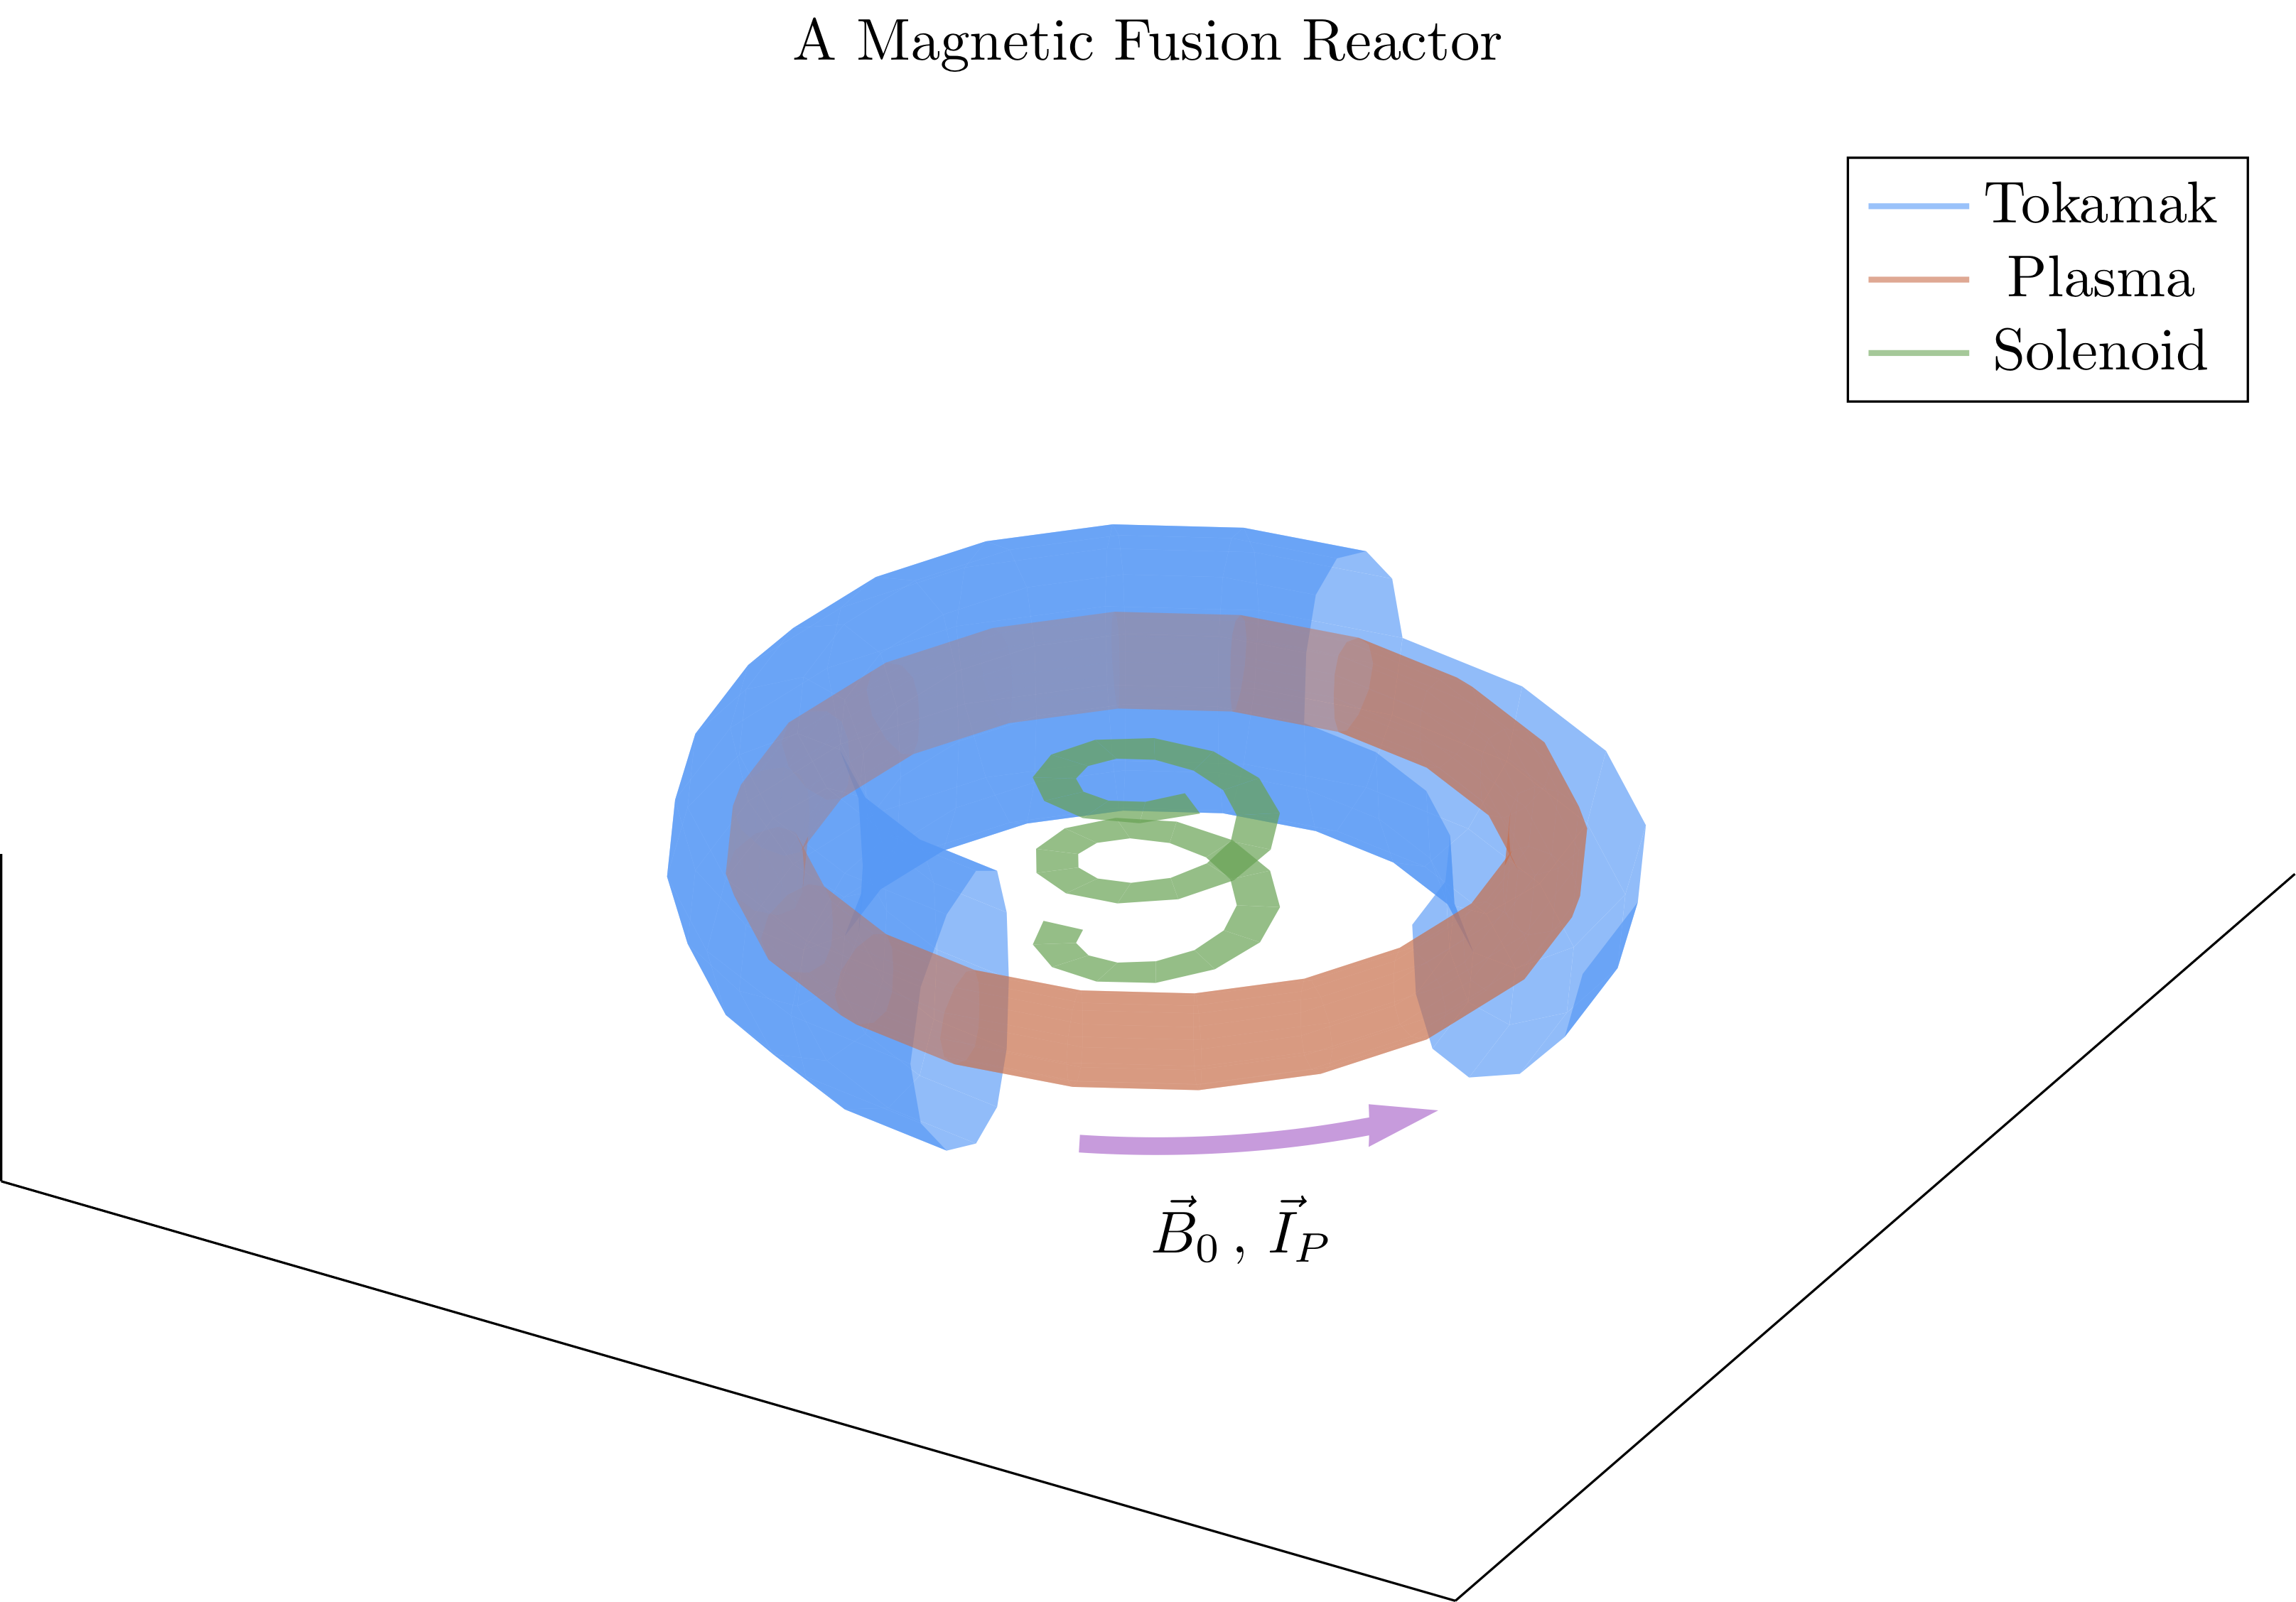
\includegraphics[width=0.75\textwidth]{images/fusion_reactor}
	\caption{Cut-Away of Tokamak Reactor} ~\\
	\small The three main components of a magnetic fusion reactor are: the tokamak structure, the plasma fuel, and the spring-like solenoid at the center.
\end{figure}

A tokamak is one of the leading candidates for a profitable fusion reactor. It shares the shape of a doughnut, using magnets to keep a hula hoop of plasma swirling inside it. The difficulty of keeping this plasma swirling though, is that it does not enjoy being spun too fast or squeezed too hard. Conversely, the tokamak housing the plasma does not like taking too much of a beating or being scaled to T-Rex sized proportions. This sets the stage for tokamak reactor design -- building on the various plasma physics and nuclear engineering constraints of the day. 

One of the most contentious points of building a tokamak, however, is whether it will be run as: pulsed (the European approach \cite{eupulsed}) or steady-state (the United States effort \cite{ussteady}). Here, pulsed operation refers to how a reactor is turned on and off periodically -- around ten times a day. Whereas, steady state machines are meant to be left on nearly the entirety of their 50-year campaigns. These behaviors are shown in \cref{fig:pulses}.

\begin{figure}
	\centering
	\begin{adjustbox}{width=0.75\textwidth}
		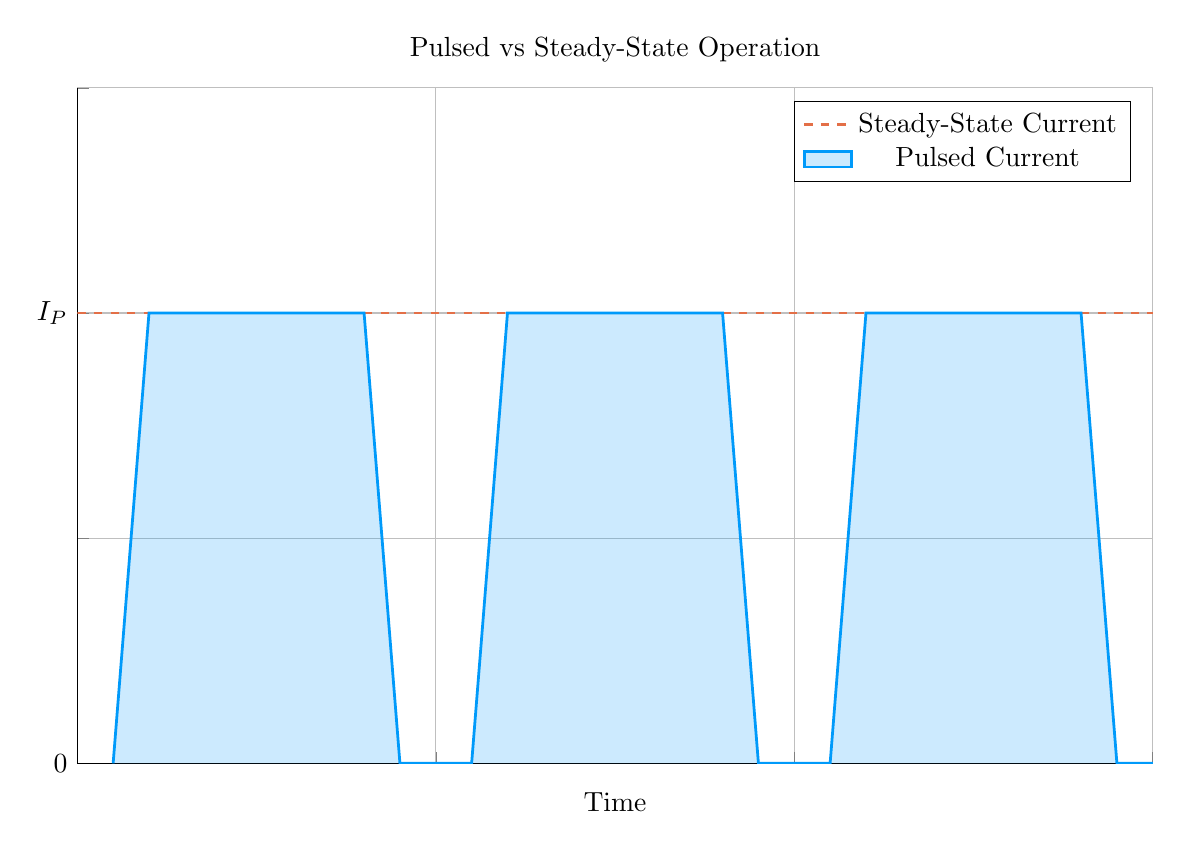
\begin{tikzpicture}[]
\begin{axis}[height = {101.6mm}, ylabel = {}, title = {Pulsed vs Steady-State Operation}, xmin = {0}, xmax = {30}, ymax = {1.5}, xlabel = {Time}, {unbounded coords=jump, scaled x ticks = false, xticklabel style={rotate = 0}, xmajorgrids = true, xtick = {10,20,30}, xticklabels = {}, xtick align = inside, axis lines* = left, scaled y ticks = false, yticklabel style={rotate = 0}, ymajorgrids = true, ytick = {0.0,0.5,1.0,1.5}, yticklabels = {0,,$I_P$,}, ytick align = inside, axis lines* = left,     xshift = 0.0mm,
    yshift = 0.0mm,
    axis background/.style={fill={rgb,1:red,1.00000000;green,1.00000000;blue,1.00000000}}
}, ymin = {0}, width = {152.4mm}]\addplot+ [color = {rgb,1:red,0.88887350;green,0.43564919;blue,0.27812294},
draw opacity=1.0,
line width=1,
dashed,mark = none,
mark size = 2.0,
mark options = {
    color = {rgb,1:red,0.00000000;green,0.00000000;blue,0.00000000}, draw opacity = 1.0,
    fill = {rgb,1:red,0.88887350;green,0.43564919;blue,0.27812294}, fill opacity = 1.0,
    line width = 1,
    rotate = 0,
    solid
}]coordinates {
(0.0, 1.0)
(2.0, 1.0)
(NaN, NaN)
(8.0, 1.0)
(12.0, 1.0)
(NaN, NaN)
(18.0, 1.0)
(22.0, 1.0)
(NaN, NaN)
(28.0, 1.0)
(30.0, 1.0)
};
\addlegendentry{Steady-State Current}
\addplot+ [color = {rgb,1:red,0.00000000;green,0.60560316;blue,0.97868012},
draw opacity=1.0,
line width=1,
solid,mark = none,
mark size = 2.0,
mark options = {
    color = {rgb,1:red,0.00000000;green,0.00000000;blue,0.00000000}, draw opacity = 1.0,
    fill = {rgb,1:red,0.00000000;green,0.60560316;blue,0.97868012}, fill opacity = 1.0,
    line width = 1,
    rotate = 0,
    solid
},fill = {rgb,1:red,0.00000000;green,0.60560316;blue,0.97868012}, fill opacity=0.2,area legend]coordinates {
(1, 0)
(2, 1)
(8, 1)
(9, 0)
(11, 0)
(11, 0)
(12, 1)
(18, 1)
(19, 0)
(21, 0)
(21, 0)
(22, 1)
(28, 1)
(29, 0)
(31, 0)
};
\addlegendentry{Pulsed Current}
\end{axis}

\end{tikzpicture}

	\end{adjustbox}
%	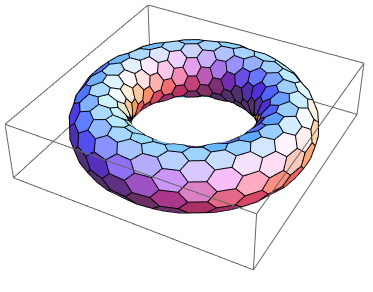
\includegraphics[width=0.85\textwidth]{images/test_image}
	\caption{Comparison of Pulsed and Steady-State Current} ~\\
	\small Inside a pulsed reactor, current is ramped up and down several times a day -- with breaks in-between. Steady state reactors are meant to stay on for weeks, months, or years.
	\label{fig:pulses}
\end{figure}

These two modes of operation, \emph{pulsed} and \emph{steady-state}, greatly influence the design through the current balance equation (derived later). What this means practically is tokamaks need current to spin their plasma hoops at some required speed and this current has to come from somewhere. Luckily, the plasma naturally enjoys spinning and provides some assistance through the bootstrap current. The remaining current must then be produced by external means.

The source of external current drive is what distinguishes pulsed from steady-state devices. Steady-state devices provide the required current assistance either through lasers or particle beams -- this paper's model focusing on a type of laser assistance called lower-hybrid current drive (LHCD). \cite{jeff} Pulsed machines, on the other hand, rely on inductive sources -- which by definition require cycles of charging and discharging several times a day.\footnote{ These inductive sources are akin to a battery on a laptop that must be recharged every so often. }

The goal of this document is to show that pulsed and steady-state operation are actually two sides of the same coin. This yields the simple conclusion that a single comprehensive model can run both modes at the flip of a switch. It even opens the opportunity of a hybrid reactor that exists somewhere in between the two.

\section{Treating Fusion as a Business}

Plasmas may be interesting, but that is not why countries build billion dollar research experiments. The ultimate goal of fusion research is to develop an energy resource that competes with coal and other base-load power sources (e.g.\ from hydroelectric and nuclear fission power plants). The problem is plasmas are chaotic and hard to contain, while tokamaks are expensive and slow to build. This perfect match has long put the field's projected timeline to that of \emph{fusion never}. \cite{fusionfunding}

\begin{figure}[h]
	\centering
	\begin{adjustbox}{width=0.75\textwidth}
		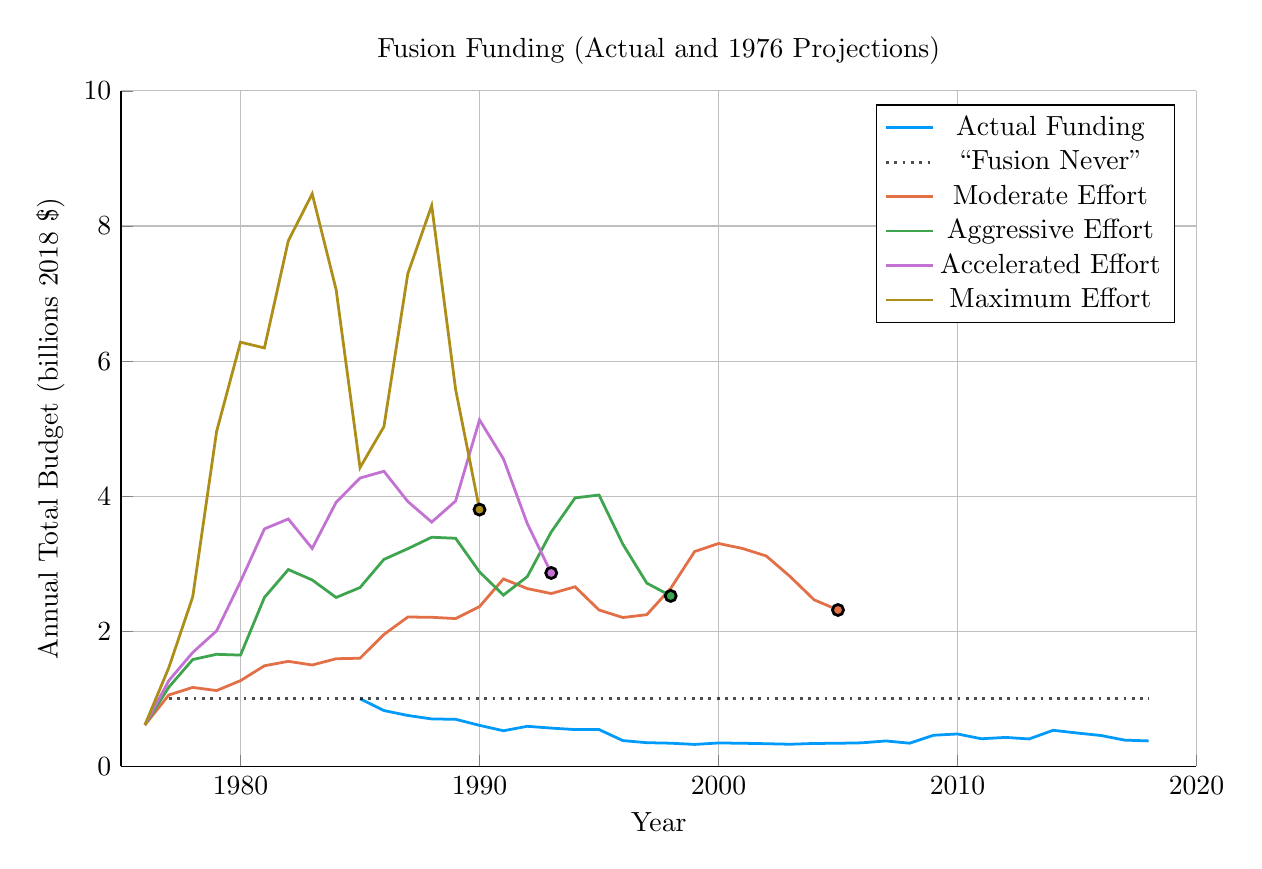
\begin{tikzpicture}[]
\begin{axis}[height = {101.6mm}, ylabel = {Annual Total Budget (billions 2018 \$)}, title = {Fusion Funding (Actual and 1976 Projections)}, xmin = {1975}, xmax = {2020}, ymax = {10}, xlabel = {Year}, {unbounded coords=jump, scaled x ticks = false, xticklabel style={rotate = 0}, xmajorgrids = true, xtick = {1980.0,1990.0,2000.0,2010.0,2020.0}, xticklabels = {1980,1990,2000,2010,2020}, xtick align = inside, axis lines* = left, scaled y ticks = false, yticklabel style={rotate = 0}, ymajorgrids = true, ytick = {0.0,2.0,4.0,6.0,8.0,10.0}, yticklabels = {0,2,4,6,8,10}, ytick align = inside, axis lines* = left,     xshift = 0.0mm,
    yshift = 0.0mm,
    axis background/.style={fill={rgb,1:red,1.00000000;green,1.00000000;blue,1.00000000}}
}, ymin = {0}, width = {152.4mm}]\addplot+ [color = {rgb,1:red,0.00000000;green,0.60560316;blue,0.97868012},
draw opacity=1.0,
line width=1,
solid,mark = none,
mark size = 2.0,
mark options = {
    color = {rgb,1:red,0.00000000;green,0.00000000;blue,0.00000000}, draw opacity = 1.0,
    fill = {rgb,1:red,0.00000000;green,0.60560316;blue,0.97868012}, fill opacity = 1.0,
    line width = 1,
    rotate = 0,
    solid
}]coordinates {
(1985.0, 1.001836)
(1986.0, 0.827367)
(1987.0, 0.754179)
(1988.0, 0.702929)
(1989.0, 0.697497)
(1990.0, 0.608102)
(1991.0, 0.527899)
(1992.0, 0.593976)
(1993.0, 0.567297)
(1994.0, 0.545463)
(1995.0, 0.545963)
(1996.0, 0.382175)
(1997.0, 0.351267)
(1998.0, 0.343818)
(1999.0, 0.325482)
(2000.0, 0.347117)
(2001.0, 0.342814)
(2002.0, 0.336267)
(2003.0, 0.32825)
(2004.0, 0.339832)
(2005.0, 0.342925)
(2006.0, 0.349302)
(2007.0, 0.377075)
(2008.0, 0.343662)
(2009.0, 0.461341)
(2010.0, 0.48051)
(2011.0, 0.409602)
(2012.0, 0.42938)
(2013.0, 0.406833)
(2014.0, 0.534818)
(2015.0, 0.494834)
(2016.0, 0.457833)
(2017.0, 0.389125)
(2018.0, 0.377419)
};
\addlegendentry{Actual Funding}
\addplot+ [color = {rgb,1:red,0.00000000;green,0.00000000;blue,0.00000000},
draw opacity=0.7,
line width=1,
dotted,mark = none,
mark size = 2.0,
mark options = {
    color = {rgb,1:red,0.00000000;green,0.00000000;blue,0.00000000}, draw opacity = 0.7,
    fill = {rgb,1:red,0.00000000;green,0.00000000;blue,0.00000000}, fill opacity = 0.7,
    line width = 1,
    rotate = 0,
    solid
}]coordinates {
(1977, 1)
(2018, 1)
};
\addlegendentry{``Fusion Never''}
\addplot+ [color = {rgb,1:red,0.88887350;green,0.43564919;blue,0.27812294},
draw opacity=1.0,
line width=1,
solid,mark = none,
mark size = 2.0,
mark options = {
    color = {rgb,1:red,0.00000000;green,0.00000000;blue,0.00000000}, draw opacity = 1.0,
    fill = {rgb,1:red,0.88887350;green,0.43564919;blue,0.27812294}, fill opacity = 1.0,
    line width = 1,
    rotate = 0,
    solid
}]coordinates {
(1976.0, 0.61374)
(1977.0, 1.05764)
(1978.0, 1.1695799999999998)
(1979.0, 1.12326)
(1980.0, 1.2699399999999998)
(1981.0, 1.48996)
(1982.0, 1.55558)
(1983.0, 1.5015399999999999)
(1984.0, 1.59418)
(1985.0, 1.6018999999999999)
(1986.0, 1.9531599999999998)
(1987.0, 2.2117799999999996)
(1988.0, 2.2079199999999997)
(1989.0, 2.18862)
(1990.0, 2.36618)
(1991.0, 2.77534)
(1992.0, 2.63252)
(1993.0, 2.55918)
(1994.0, 2.65954)
(1995.0, 2.316)
(1996.0, 2.2040599999999997)
(1997.0, 2.24652)
(1998.0, 2.63638)
(1999.0, 3.18064)
(2000.0, 3.3002999999999996)
(2001.0, 3.2269599999999996)
(2002.0, 3.11502)
(2003.0, 2.8100799999999997)
(2004.0, 2.4665399999999997)
(2005.0, 2.316)
};
\addlegendentry{Moderate Effort}
\addplot+[draw=none, color = {rgb,1:red,0.88887350;green,0.43564919;blue,0.27812294},
draw opacity=1.0,
line width=0,
solid,mark = *,
mark size = 2.0,
mark options = {
    color = {rgb,1:red,0.00000000;green,0.00000000;blue,0.00000000}, draw opacity = 1.0,
    fill = {rgb,1:red,0.88887350;green,0.43564919;blue,0.27812294}, fill opacity = 1.0,
    line width = 1,
    rotate = 0,
    solid
},forget plot] coordinates {
(2005.0, 2.316)
};
\addplot+ [color = {rgb,1:red,0.24222430;green,0.64327509;blue,0.30444865},
draw opacity=1.0,
line width=1,
solid,mark = none,
mark size = 2.0,
mark options = {
    color = {rgb,1:red,0.00000000;green,0.00000000;blue,0.00000000}, draw opacity = 1.0,
    fill = {rgb,1:red,0.24222430;green,0.64327509;blue,0.30444865}, fill opacity = 1.0,
    line width = 1,
    rotate = 0,
    solid
}]coordinates {
(1976.0, 0.61374)
(1977.0, 1.1734399999999998)
(1978.0, 1.5825999999999998)
(1979.0, 1.6598)
(1980.0, 1.6482199999999998)
(1981.0, 2.50128)
(1982.0, 2.9143)
(1983.0, 2.7598999999999996)
(1984.0, 2.50128)
(1985.0, 2.64796)
(1986.0, 3.06484)
(1987.0, 3.2230999999999996)
(1988.0, 3.39294)
(1989.0, 3.3775)
(1990.0, 2.8795599999999997)
(1991.0, 2.5360199999999997)
(1992.0, 2.8100799999999997)
(1993.0, 3.47014)
(1994.0, 3.9757999999999996)
(1995.0, 4.01826)
(1996.0, 3.2887199999999996)
(1997.0, 2.71358)
(1998.0, 2.52444)
};
\addlegendentry{Aggressive Effort}
\addplot+[draw=none, color = {rgb,1:red,0.24222430;green,0.64327509;blue,0.30444865},
draw opacity=1.0,
line width=0,
solid,mark = *,
mark size = 2.0,
mark options = {
    color = {rgb,1:red,0.00000000;green,0.00000000;blue,0.00000000}, draw opacity = 1.0,
    fill = {rgb,1:red,0.24222430;green,0.64327509;blue,0.30444865}, fill opacity = 1.0,
    line width = 1,
    rotate = 0,
    solid
},forget plot] coordinates {
(1998.0, 2.52444)
};
\addplot+ [color = {rgb,1:red,0.76444018;green,0.44411178;blue,0.82429754},
draw opacity=1.0,
line width=1,
solid,mark = none,
mark size = 2.0,
mark options = {
    color = {rgb,1:red,0.00000000;green,0.00000000;blue,0.00000000}, draw opacity = 1.0,
    fill = {rgb,1:red,0.76444018;green,0.44411178;blue,0.82429754}, fill opacity = 1.0,
    line width = 1,
    rotate = 0,
    solid
}]coordinates {
(1976.0, 0.61374)
(1977.0, 1.2699399999999998)
(1978.0, 1.68682)
(1979.0, 2.0071999999999997)
(1980.0, 2.7367399999999997)
(1981.0, 3.51646)
(1982.0, 3.66314)
(1983.0, 3.2269599999999996)
(1984.0, 3.9101799999999995)
(1985.0, 4.269159999999999)
(1986.0, 4.36952)
(1987.0, 3.92176)
(1988.0, 3.6168199999999997)
(1989.0, 3.92948)
(1990.0, 5.1299399999999995)
(1991.0, 4.554799999999999)
(1992.0, 3.59366)
(1993.0, 2.8641199999999998)
};
\addlegendentry{Accelerated Effort}
\addplot+[draw=none, color = {rgb,1:red,0.76444018;green,0.44411178;blue,0.82429754},
draw opacity=1.0,
line width=0,
solid,mark = *,
mark size = 2.0,
mark options = {
    color = {rgb,1:red,0.00000000;green,0.00000000;blue,0.00000000}, draw opacity = 1.0,
    fill = {rgb,1:red,0.76444018;green,0.44411178;blue,0.82429754}, fill opacity = 1.0,
    line width = 1,
    rotate = 0,
    solid
},forget plot] coordinates {
(1993.0, 2.8641199999999998)
};
\addplot+ [color = {rgb,1:red,0.67554396;green,0.55566233;blue,0.09423434},
draw opacity=1.0,
line width=1,
solid,mark = none,
mark size = 2.0,
mark options = {
    color = {rgb,1:red,0.00000000;green,0.00000000;blue,0.00000000}, draw opacity = 1.0,
    fill = {rgb,1:red,0.67554396;green,0.55566233;blue,0.09423434}, fill opacity = 1.0,
    line width = 1,
    rotate = 0,
    solid
}]coordinates {
(1976.0, 0.61374)
(1977.0, 1.46294)
(1978.0, 2.509)
(1979.0, 4.9601)
(1980.0, 6.28022)
(1981.0, 6.1953)
(1982.0, 7.781759999999999)
(1983.0, 8.47656)
(1984.0, 7.059939999999999)
(1985.0, 4.423559999999999)
(1986.0, 5.029579999999999)
(1987.0, 7.2954)
(1988.0, 8.302859999999999)
(1989.0, 5.58156)
(1990.0, 3.8021)
};
\addlegendentry{Maximum Effort}
\addplot+[draw=none, color = {rgb,1:red,0.67554396;green,0.55566233;blue,0.09423434},
draw opacity=1.0,
line width=0,
solid,mark = *,
mark size = 2.0,
mark options = {
    color = {rgb,1:red,0.00000000;green,0.00000000;blue,0.00000000}, draw opacity = 1.0,
    fill = {rgb,1:red,0.67554396;green,0.55566233;blue,0.09423434}, fill opacity = 1.0,
    line width = 1,
    rotate = 0,
    solid
},forget plot] coordinates {
(1990.0, 3.8021)
};
\end{axis}

\end{tikzpicture}

	\end{adjustbox}
%	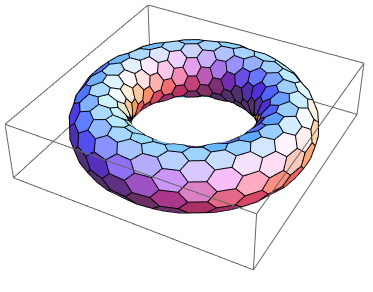
\includegraphics[width=0.75\textwidth]{images/test_image}
	\caption{Fusion Never Funding Timeline} ~\\
	\small Comparison of Projected Timelines of Fusion from 1976 with Actual DOE Budgets. \cite{doe87, doe19} \\ The dotted line is popularly referred to in the community as ``Fusion Never.'' \cite{fusionnever}
\end{figure}

The major problem with containing a plasma in a reactor is that a plasma does not want to be contained. Since the early days of fusion research, plasmas have often found escape mechanisms. When presented with a magnetic bottle, they found their way out the top. In a tokamak, they attack the outer edges like an overinflated tire-tube. Fusion energy has seemed to remain a Tantalizing effort -- within arms reach, but staunchly guarded by a shroud of instabilities.

The truth is plasmas are extremely chaotic: they show nonlinear behavior in almost everything they do. As of now, no theory or supercomputer-backed code can predict even something so fundamental to design as the movement of energy and particles within a tokamak. As such, the field has adopted several rules of thumb and empirical scalings -- based on the last half century of experiments -- which help one navigate around a plasma's finicky behavior.

The two most widely used rules of thumb within the fusion design community are: the Greenwald density limit and the ELMy H-Mode confinement time scaling law. As such, the model in this document heavily utilizes the two to make a quick running code. These two relations are also why this model -- which happens to be zero-dimensional -- can reproduce with high fidelity the answers from three-dimensional codes, which can take days, weeks, or even months to run!

\begin{figure}
	\centering
	\begin{adjustbox}{width=0.75\textwidth}
		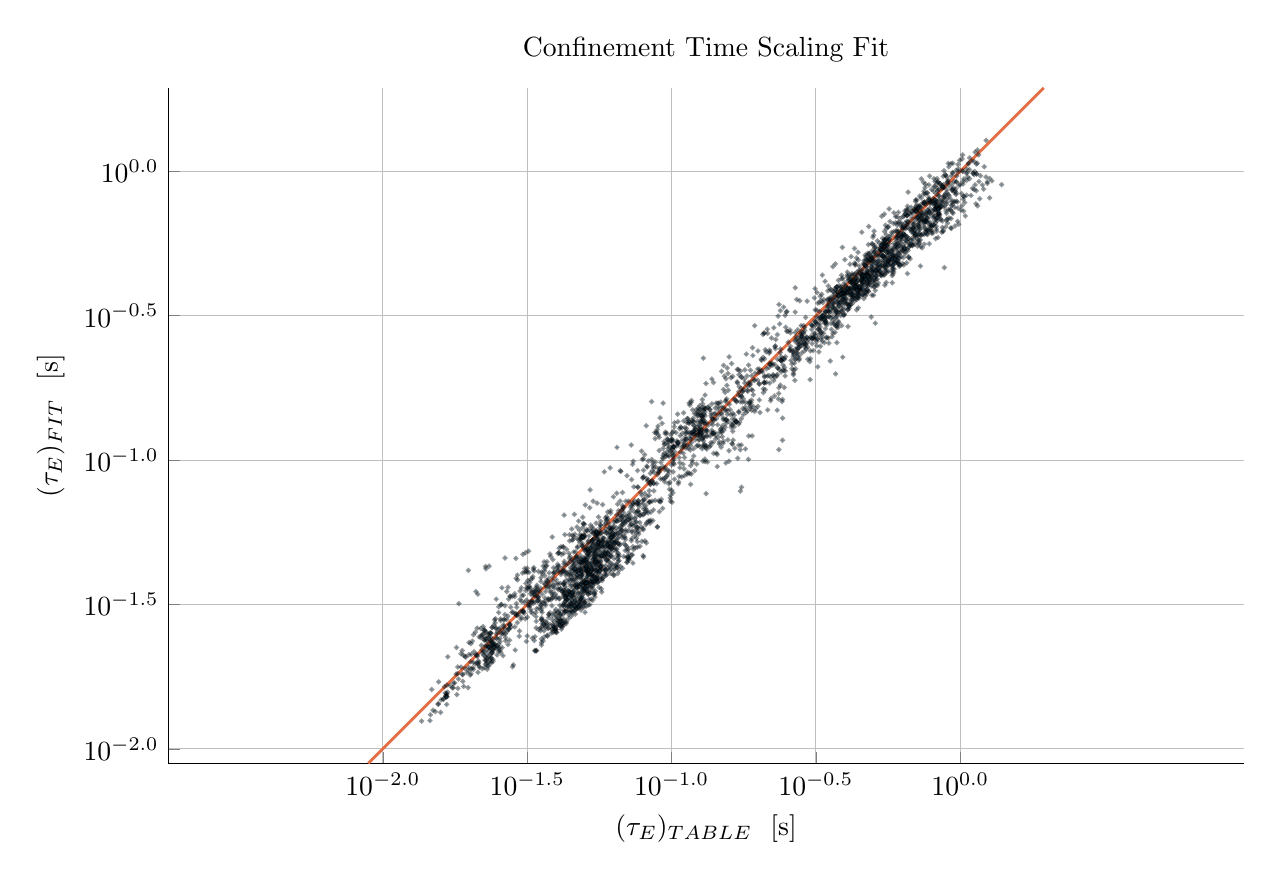
\begin{tikzpicture}[]
\begin{axis}[height = {101.6mm}, axis equal = {true}, ylabel = {$(\tau_E)_{ FIT } \ \ [ \textnormal{s} ]$}, title = {Confinement Time Scaling Fit}, xmin = {0.008904842990761705}, xmax = {1.9473999999999996}, ymax = {1.9473999999999996}, ymode = {log}, xlabel = {$(\tau_E)_{ TABLE } \ \ [ \textnormal{s} ]$}, {unbounded coords=jump, scaled x ticks = false, xticklabel style={rotate = 0}, log basis x=10, xmajorgrids = true, xtick = {0.01,0.03162277660168379,0.1,0.31622776601683794,1.0}, xticklabels = {$10^{-2.0}$,$10^{-1.5}$,$10^{-1.0}$,$10^{-0.5}$,$10^{0.0}$}, xtick align = inside, axis lines* = left, scaled y ticks = false, yticklabel style={rotate = 0}, log basis y=10, ymajorgrids = true, ytick = {0.01,0.03162277660168379,0.1,0.31622776601683794,1.0}, yticklabels = {$10^{-2.0}$,$10^{-1.5}$,$10^{-1.0}$,$10^{-0.5}$,$10^{0.0}$}, ytick align = inside, axis lines* = left,     xshift = 0.0mm,
    yshift = 0.0mm,
    axis background/.style={fill={rgb,1:red,1.00000000;green,1.00000000;blue,1.00000000}}
}, xmode = {log}, ymin = {0.008904842990761705}, width = {152.4mm}]\addplot+[draw=none, color = {rgb,1:red,0.00000000;green,0.60560316;blue,0.97868012},
draw opacity=0.4,
line width=0,
solid,mark = *,
mark size = 0.325,
mark options = {
    color = {rgb,1:red,0.00000000;green,0.00000000;blue,0.00000000}, draw opacity = 0.4,
    fill = {rgb,1:red,0.00000000;green,0.60560316;blue,0.97868012}, fill opacity = 0.4,
    line width = 1,
    rotate = 0,
    solid
},forget plot] coordinates {
(0.048709999999999996, 0.03286927009465151)
(0.047479999999999994, 0.030718782340371346)
(0.056709999999999997, 0.04427687673230967)
(0.06154, 0.040523205193333994)
(0.049249999999999995, 0.031000215657666388)
(0.046439999999999995, 0.03902384637413358)
(0.04536, 0.03366158264691253)
(0.041229999999999996, 0.029311430641277475)
(0.04224, 0.03489492877112558)
(0.05357, 0.03985677848149215)
(0.042449999999999995, 0.030139467297048302)
(0.04393, 0.03525642598465171)
(0.037579999999999995, 0.029115058174186102)
(0.040589999999999994, 0.03552938448965956)
(0.016339999999999997, 0.016414220556232706)
(0.01926, 0.018966660638066977)
(0.014769999999999998, 0.01604916788911629)
(0.020909999999999998, 0.019687625330862386)
(0.014559999999999998, 0.01252323235667468)
(0.016659999999999998, 0.016615842361327)
(0.017099999999999997, 0.016562775820865377)
(0.025429999999999998, 0.024119656293897448)
(0.01834, 0.03183654298531315)
(0.02225, 0.026522518089311862)
(0.02354, 0.023762954142859543)
(0.01883, 0.02190554572449257)
(0.0156, 0.0170549295762654)
(0.01678, 0.020822704009415233)
(0.154, 0.14943255990407037)
(0.17639999999999997, 0.1506224447310805)
(0.7525999999999999, 0.7841653529419872)
(0.7196999999999999, 0.7123510444198007)
(0.7581, 0.7126653992395249)
(0.5971, 0.6636747785042374)
(0.5545, 0.6034081737695671)
(0.5620999999999999, 0.5855426425362842)
(0.7231, 0.611757051674103)
(0.7314999999999999, 0.6000776436052295)
(0.8261999999999999, 0.7332080576221435)
(0.8526999999999999, 0.6874473851854792)
(0.7659999999999999, 0.6249854199535853)
(0.8212999999999999, 0.6647675128338589)
(0.7968, 0.6202645990011652)
(1.1369999999999998, 0.8572954951071405)
(0.8379, 0.709498458538988)
(0.7112999999999999, 0.6481476339591892)
(0.8383999999999999, 0.7100253242029977)
(0.9772, 0.7850517774047457)
(0.6932999999999999, 0.6449986085844157)
(0.7078, 0.5696128161569505)
(0.7666999999999999, 0.6076651618162499)
(0.7231, 0.8218656209469912)
(0.7654, 0.7824204839027497)
(0.8880999999999999, 0.9751544259782554)
(0.9436, 0.987045215482296)
(0.982, 1.0567556111003251)
(1.0659999999999998, 1.0600221351309262)
(1.021, 1.0023421135083617)
(1.037, 0.780421246365204)
(1.0139999999999998, 0.7598649860996711)
(0.9391999999999999, 0.722374477345195)
(0.7876, 0.7737488110528499)
(0.7564, 0.8355652777917266)
(0.8073999999999999, 0.7829615268340135)
(0.6101, 0.662119064106307)
(0.5015, 0.6015695673902948)
(0.7323999999999999, 0.8090796506003152)
(0.6535, 0.7394639493973881)
(0.5972, 0.6975536633839833)
(0.8778999999999999, 0.7874999827504517)
(0.7773, 0.8125562886500788)
(0.6810999999999999, 0.7238692523345119)
(0.6392, 0.701072652615907)
(0.6046999999999999, 0.6507248504722397)
(0.9085, 1.0662323587837632)
(0.746, 0.9171741777262944)
(0.6601999999999999, 0.8477587902173862)
(1.019, 1.1402820961295275)
(0.9123, 1.0371038527895822)
(0.5081, 0.5255375119481419)
(0.7402, 0.6843189302449205)
(0.7313999999999999, 0.6912025500896107)
(1.0779999999999998, 1.1138270195034614)
(0.6314, 0.6309700937894861)
(0.9303999999999999, 0.9647835607071941)
(0.8503, 0.9084098651600415)
(0.8125, 0.8871934724039697)
(0.9943, 1.0920838325900788)
(0.8109999999999999, 0.94316240550339)
(0.7583, 0.9027068941508603)
(0.8357, 0.9197400869136341)
(0.6762999999999999, 0.7509390530838264)
(0.6529999999999999, 0.7031904860947172)
(0.3892, 0.34318485870648646)
(0.34049999999999997, 0.3124029593731834)
(0.45299999999999996, 0.3908324185235881)
(0.44149999999999995, 0.37445805641759866)
(0.5680999999999999, 0.519309036063986)
(0.5427, 0.470258508275619)
(0.3973, 0.3208880474419727)
(0.4023, 0.3620545624474692)
(0.36279999999999996, 0.3723269788644909)
(0.5475, 0.4394327211967968)
(0.3898, 0.37922457801357046)
(0.31279999999999997, 0.303118325347936)
(0.38389999999999996, 0.35281373501460195)
(0.3181, 0.31386085182034285)
(0.7142, 0.6930925801653104)
(0.6252, 0.6626568011479417)
(0.6154999999999999, 0.5263153459242683)
(0.9141999999999999, 0.6902582143865932)
(0.7587999999999999, 0.6215886466745869)
(0.6337999999999999, 0.5997015869390643)
(0.9221999999999999, 0.7382203149764545)
(0.6928, 0.6177290812059213)
(0.7125999999999999, 0.6963967594591091)
(0.21899999999999997, 0.18496435234301067)
(0.20789999999999997, 0.1766203805469118)
(0.26499999999999996, 0.20490261922028621)
(0.4225, 0.34891440428748743)
(0.4118, 0.3421446077261888)
(0.2397, 0.22159945467095882)
(0.26959999999999995, 0.22409261472703068)
(0.3127, 0.2631427459860977)
(0.32389999999999997, 0.2832737570128158)
(0.8515999999999999, 0.9068928303444452)
(0.8177, 0.9220516908419841)
(1.0179999999999998, 1.002889177259622)
(0.5892999999999999, 0.7186483132855688)
(0.9675999999999999, 0.918899482262656)
(0.8809999999999999, 0.4645188486258639)
(1.077, 1.013495270683344)
(0.5667, 0.7415870515780109)
(0.5344, 0.6992580529977903)
(0.5457, 0.7114200487063042)
(0.6599999999999999, 0.568829584256022)
(0.7506999999999999, 0.604323636235005)
(0.7131, 0.5987909231331726)
(0.6576, 0.5815966808550769)
(0.6386, 0.6040200009888924)
(0.4816, 0.6444934910993216)
(0.45589999999999997, 0.6160051006574458)
(0.6427999999999999, 0.7305600248168257)
(0.8285999999999999, 0.7476043736628556)
(0.6534, 0.6544069370264392)
(0.6638999999999999, 0.6723198321350972)
(0.5883999999999999, 0.5629685596654105)
(0.6073999999999999, 0.5947667114406178)
(0.5639, 0.5731530731910407)
(0.6101, 0.6034835968431853)
(0.6638999999999999, 0.5863468310710566)
(0.6346999999999999, 0.5309682418246683)
(0.5062, 0.456996379113654)
(0.6548999999999999, 0.703107054401337)
(0.5526, 0.5545528151553201)
(0.8658999999999999, 0.7858011508612296)
(0.7361, 0.7026740161837454)
(0.734, 0.7080907193345652)
(0.722, 0.7026124938878728)
(0.9287, 1.0629014859458583)
(0.7698999999999999, 0.84074579772222)
(0.8176, 0.8870105921186713)
(0.5843999999999999, 0.5035404234450113)
(0.9373999999999999, 0.8698220688660848)
(0.9337, 0.8623382177770421)
(0.8964, 0.7160170198322513)
(0.7332, 0.9423078640879671)
(0.7831999999999999, 0.963224279565402)
(0.9906999999999999, 0.8952623033567918)
(0.9087, 0.8308130537672082)
(0.7955, 0.8658102097350978)
(0.9360999999999999, 0.9039593399896794)
(0.7863, 0.714131359979918)
(0.8229, 0.740299033130453)
(0.823, 0.760314511413916)
(0.7636999999999999, 0.7163144408463683)
(0.6311, 0.5556779797096207)
(0.6262, 0.6533313908678976)
(0.8946999999999999, 0.9586908006605939)
(0.8576999999999999, 0.7537146014939096)
(0.8473999999999999, 0.7461424250229518)
(0.9255, 0.801575405231461)
(0.8498, 0.7649223531344689)
(0.7823, 0.7268518889656576)
(0.8255999999999999, 0.7470872412684922)
(0.8631, 0.7753860665056598)
(0.7994, 0.728145541191726)
(0.8747999999999999, 0.8208827079316118)
(1.015, 1.1045865073889138)
(1.1609999999999998, 0.9219761380746218)
(0.7623, 0.6715119057586799)
(0.7824, 0.6467686006890678)
(0.5243, 0.564617572937227)
(0.5503999999999999, 0.5783318044105018)
(0.5407, 0.5701439812605221)
(0.5317999999999999, 0.5494542896098417)
(0.5491999999999999, 0.5670933149802504)
(0.5455, 0.5598085924937554)
(0.8478, 0.7018507562099994)
(0.7223999999999999, 0.6570441876740942)
(0.8067, 0.7135500971429034)
(0.7686999999999999, 0.6885128255514706)
(0.7448999999999999, 0.6760240646258281)
(0.7343, 0.6742929760912958)
(0.6597999999999999, 0.7354882011318915)
(0.6793999999999999, 0.7289884081681665)
(0.6546, 0.7051597393592424)
(0.9087999999999999, 0.7368656746766299)
(0.7526999999999999, 0.671806203783079)
(0.7545, 0.8781283223894364)
(0.969, 1.0091726548574242)
(0.9864999999999999, 0.9978820947672817)
(0.9519, 0.8476711232851686)
(0.8273999999999999, 0.778663500363082)
(0.8248, 0.7801934517664398)
(0.6835, 0.6627837535553688)
(0.6928, 0.6114247462326845)
(0.7931999999999999, 0.6269714335560767)
(0.7208, 0.6045147201505461)
(0.6963999999999999, 0.6028585041743847)
(0.8253999999999999, 0.6317543998575686)
(0.6675, 0.5602136085491106)
(0.7319, 0.6026263780884397)
(0.6533, 0.5360321914526158)
(0.564, 0.4904554472531542)
(0.9439, 0.7157171194446946)
(0.7939999999999999, 0.6411620402371146)
(0.8091999999999999, 0.6525781912908896)
(0.7292, 0.5485933677696657)
(0.6357999999999999, 0.503286345980577)
(0.6447999999999999, 0.5185162967617107)
(1.069, 1.0695180372896376)
(0.8583, 0.8908809768320126)
(0.8087, 0.8543034142940075)
(0.8318, 0.9446369769051516)
(0.7786, 0.8979525071302351)
(1.1219999999999999, 0.9996281574893591)
(1.107, 0.9853860242113884)
(1.2109999999999999, 1.0380777356700828)
(1.109, 0.988185626984255)
(0.8967999999999999, 0.7722301840545289)
(0.824, 0.8390911317907782)
(0.8246, 0.7494173273698013)
(0.7246999999999999, 0.6803976433290927)
(0.6926, 0.6607682224597816)
(0.8103999999999999, 0.7710346210832281)
(0.7748999999999999, 0.7325112272388337)
(0.7414999999999999, 0.7062682017319861)
(0.8249, 0.6842066249663288)
(0.8475999999999999, 0.7093971409693103)
(0.7781999999999999, 0.6302194723063099)
(0.7003999999999999, 0.6008831528899192)
(0.6518999999999999, 0.5945976708252837)
(0.7195999999999999, 0.5780911978357602)
(0.7698999999999999, 0.6045774400058568)
(0.6951999999999999, 0.5594902956731888)
(0.6265999999999999, 0.5281946682083224)
(1.0519999999999998, 0.9316449640552941)
(1.011, 0.8373271253227542)
(1.0619999999999998, 0.9564802790915702)
(0.9991, 0.8998058834673238)
(1.1019999999999999, 0.874362127898913)
(0.9502999999999999, 0.7861813492490419)
(1.1929999999999998, 0.8970574608241824)
(1.1409999999999998, 0.9798783118539908)
(1.1389999999999998, 0.981247441890904)
(0.7454, 0.6506062999832742)
(0.7213999999999999, 0.6316980480914915)
(0.7511, 0.6382470829505086)
(1.168, 0.8045488413734408)
(1.1329999999999998, 0.7723998453123871)
(1.2049999999999998, 0.8686731269524)
(0.8418, 0.7105640304650586)
(0.8438, 0.7167529167481481)
(0.8319, 0.6761440014142099)
(0.7971999999999999, 0.647212185326572)
(0.8099999999999999, 0.6507837939912798)
(0.954, 0.7838744415871535)
(1.0279999999999998, 0.8191939822720388)
(1.029, 0.8188141254422304)
(0.9371999999999999, 0.765214397024378)
(1.0219999999999998, 0.9050020965486358)
(1.1449999999999998, 1.0674931488210169)
(1.136, 1.0609598989430766)
(0.9721, 0.9642173576087313)
(0.8966, 0.8641697646781274)
(0.8880999999999999, 0.8373748291165626)
(0.8997999999999999, 0.8442042621804475)
(1.0219999999999998, 0.9220333467704045)
(1.126, 0.897657994702853)
(1.2879999999999998, 0.9272527550966493)
(0.8389, 0.7182547844853155)
(0.9348, 0.7828004050235056)
(1.051, 0.8269739428545848)
(1.0239999999999998, 0.8005745674982954)
(1.158, 1.1412196875478482)
(0.8996, 0.8065770952173787)
(0.9666999999999999, 0.8315473131899693)
(0.8414999999999999, 0.7684067296642498)
(0.8493999999999999, 0.7527319188772996)
(0.8481, 0.7458196646149527)
(0.8429, 0.7423208728716764)
(0.8990999999999999, 0.7842614607464142)
(0.8253999999999999, 0.7485587864344085)
(0.8107, 0.7384132406448961)
(0.8147, 0.7410312659641048)
(0.9854999999999999, 1.0196276084818066)
(1.1469999999999998, 1.1863286392932)
(1.126, 1.1666665208852889)
(0.9404999999999999, 0.8611051902461748)
(0.7303, 0.7213915082892701)
(1.0959999999999999, 1.0877850615898468)
(1.117, 1.0833298051794935)
(1.057, 0.9923729605851154)
(0.9539, 0.9233369235535771)
(1.2289999999999999, 1.2805920757347342)
(0.8688999999999999, 0.8918437252115444)
(0.8352999999999999, 0.8716065387445937)
(0.9081999999999999, 0.9368678123602089)
(0.8755, 0.90002820580841)
(0.8695999999999999, 0.8794079728006472)
(0.8787999999999999, 0.881459737915593)
(0.9007, 0.9104206399267062)
(0.872, 0.8798842972291739)
(0.8658999999999999, 0.8749949687250976)
(0.8429, 0.8633412845042695)
(0.8341, 0.8574697533575164)
(0.7795, 0.80110995309816)
(0.8055, 0.8051314579770487)
(0.7888999999999999, 0.7871440794358052)
(0.7888, 0.78597297922507)
(0.7839999999999999, 0.783736968755363)
(0.8906999999999999, 0.9705362439027034)
(0.8353999999999999, 0.9206177853670467)
(0.9397, 0.9901636819697397)
(0.833, 0.9066645584090964)
(0.7091, 0.7411169895186779)
(0.7263999999999999, 0.7515058392068585)
(0.9071999999999999, 0.9226286568967264)
(0.8681, 0.8888136889786512)
(0.7014999999999999, 0.7549502980032216)
(0.6941999999999999, 0.7414453256597049)
(0.6193, 0.6868705118704591)
(0.7438999999999999, 0.7801456918201667)
(0.6958, 0.7373496835919023)
(0.7162, 0.7545932329675524)
(0.7295999999999999, 0.7653022211346575)
(0.7071, 0.7633267093779594)
(0.7009, 0.79841785676154)
(0.7074999999999999, 0.7960705831433198)
(0.6993999999999999, 0.7869623482126145)
(0.7202, 0.7611057495934285)
(0.7847999999999999, 0.7953466660425729)
(0.7509999999999999, 0.7704143379652046)
(0.6954999999999999, 0.7363969319361924)
(0.6666, 0.7152819454604417)
(0.7485999999999999, 0.7778447754623078)
(0.7101999999999999, 0.7347703554376556)
(0.6983999999999999, 0.7278364728917994)
(0.5580999999999999, 0.4833226862967873)
(0.6591999999999999, 0.5325006454360778)
(0.6224999999999999, 0.507999140907478)
(0.592, 0.4829571034104287)
(0.5678, 0.4750822637133591)
(0.5478999999999999, 0.46940311682153735)
(0.7485999999999999, 0.7775297709191064)
(0.7027, 0.7322537919167466)
(0.7165999999999999, 0.7453502012689315)
(0.7544, 0.7813252510105715)
(0.701, 0.7340106625957865)
(1.0499999999999998, 0.9847941321751483)
(0.7162, 0.7493085145738181)
(0.6687, 0.7135001121348747)
(0.7599999999999999, 0.768274815018355)
(0.7058, 0.7290656456829794)
(0.7031, 0.7275885380278503)
(0.7041, 0.6367181066561843)
(0.688, 0.6354802698552251)
(1.077, 0.943090689087118)
(0.9655999999999999, 0.8715157034912367)
(0.8762, 0.8088387283718785)
(0.8806999999999999, 0.8127564086172461)
(0.5542999999999999, 0.41253102576251693)
(0.5478, 0.4036039372001265)
(0.4941, 0.373031283060472)
(0.5829, 0.512947049410342)
(0.5613999999999999, 0.48664164380957775)
(0.5247999999999999, 0.4527986103525293)
(0.4695, 0.4227065708121077)
(0.48919999999999997, 0.5073610229958332)
(0.6664, 0.5504072752437238)
(0.6019, 0.506184963883185)
(0.5290999999999999, 0.46835384346341935)
(0.6813999999999999, 0.5595253856241379)
(0.5491999999999999, 0.47440537547191425)
(0.5149999999999999, 0.454161051345693)
(0.6145999999999999, 0.5153919313492221)
(0.5720999999999999, 0.48890197499449095)
(0.7011999999999999, 0.5951245600889739)
(0.6801999999999999, 0.5862584147630384)
(0.6436, 0.5779925943174439)
(0.6879, 0.6355711960485161)
(0.7161, 0.6580154715421902)
(0.6805, 0.6403947308683965)
(0.5677, 0.4994502254665087)
(0.6407999999999999, 0.537341813479382)
(0.5336, 0.4735622145714224)
(0.6022, 0.48585628016871496)
(0.5301999999999999, 0.43812776843405565)
(0.5569, 0.4511379734712108)
(0.5309999999999999, 0.4382828143980356)
(0.7189, 0.561283944496514)
(0.6033, 0.49593491486870384)
(0.5882, 0.48791409058918084)
(0.5133, 0.47086714482313546)
(0.6835, 0.5557071339364735)
(0.5457, 0.4595648149111282)
(0.5548, 0.46523133962452173)
(0.47969999999999996, 0.4249658620586939)
(0.4523, 0.415295964493189)
(0.6022, 0.5400209296818028)
(0.5538, 0.5052764641657136)
(0.5436, 0.5055194776119623)
(0.6782999999999999, 0.6163137196828592)
(0.695, 0.6266243673269388)
(0.62, 0.5813674172258797)
(0.6432, 0.5431537583550402)
(0.6287999999999999, 0.5349480622390502)
(0.6376, 0.54586058250559)
(0.5668, 0.4914002086290934)
(0.5511999999999999, 0.47842606650822395)
(0.5179999999999999, 0.4490979395028368)
(0.4926, 0.43740028298001615)
(0.45459999999999995, 0.4189036373559835)
(0.6536, 0.5941545657972782)
(0.5829, 0.5349527992919924)
(0.18815494499765392, 0.1581399078244611)
(0.2146061814556331, 0.19572896069781145)
(0.16599999999999998, 0.13799498658430565)
(0.18969999999999998, 0.14876546786696357)
(0.1833, 0.1482841294703696)
(0.1813, 0.14622039951602703)
(0.17729999999999999, 0.14361309282173648)
(0.1793, 0.14932396239540086)
(0.16018654635778376, 0.14375168149593862)
(0.23608148464163825, 0.20618864049175167)
(0.15090505517866634, 0.13993845766847318)
(0.16462308753545907, 0.14319802218703614)
(0.22867658825412063, 0.2432843316035902)
(0.15437048917401763, 0.19150835096181462)
(0.204407884525842, 0.2234568824525145)
(0.3385921358212541, 0.25515688094639516)
(0.30803062388011077, 0.2920590580475614)
(0.3698439872088892, 0.1989826760084809)
(0.3020055284361583, 0.1900834656284462)
(0.391747288185283, 0.22739364529660014)
(0.18722432262129804, 0.1513418397949884)
(0.35449272544635624, 0.220335621447283)
(0.23145587735894824, 0.1958237725659035)
(0.22568075547813332, 0.1966426493637936)
(0.12419999999999999, 0.12535236963339896)
(0.1362, 0.12116477109254274)
(0.1686, 0.18668565060566708)
(0.2571, 0.24065324034899624)
(0.14309999999999998, 0.10574864224466833)
(0.1001, 0.07861924902447287)
(0.1394, 0.11523665402006138)
(0.13169999999999998, 0.11054302384899538)
(0.1679, 0.16024914750084338)
(0.1679, 0.1592375423514523)
(0.1379, 0.1269124989160874)
(0.13759999999999997, 0.13474346567467413)
(0.15669999999999998, 0.11752104464678922)
(0.1634, 0.11731413030603775)
(0.1513, 0.11615944954854357)
(0.1641, 0.1342046675569159)
(0.1324, 0.11202070716494673)
(0.144, 0.10455225164776064)
(0.08367999999999999, 0.07550572887234856)
(0.08138, 0.06960465607403137)
(0.07985999999999999, 0.06790024415870552)
(0.06914, 0.06133434654420463)
(0.07455999999999999, 0.0659594636095902)
(0.06749, 0.059094960344554005)
(0.07956999999999999, 0.06457109181522346)
(0.07042, 0.06434532605690742)
(0.1243, 0.11740776302358609)
(0.1098, 0.10570841747417169)
(0.11209999999999999, 0.10998875997985506)
(0.12769999999999998, 0.10957807347983331)
(0.10719999999999999, 0.1065573371040371)
(0.13019999999999998, 0.11151703529901563)
(0.11929999999999999, 0.10336177621901224)
(0.18949999999999997, 0.16142608123554003)
(0.13319999999999999, 0.0985814769637825)
(0.122, 0.12133203045600598)
(0.13249999999999998, 0.12167416353208241)
(0.1772, 0.16311084283670516)
(0.11599999999999999, 0.12343156692499643)
(0.118, 0.12364896689819536)
(0.14439999999999997, 0.13258051012966407)
(0.08478999999999999, 0.06604715398119469)
(0.06265, 0.05571638354031536)
(0.06549999999999999, 0.05587664803721788)
(0.07185, 0.06281229971832496)
(0.09925999999999999, 0.07568059816491898)
(0.08231, 0.06687006216262115)
(0.10619999999999999, 0.08785115077712564)
(0.12229999999999999, 0.11192205816899478)
(0.11739999999999999, 0.11521568056327589)
(0.12789999999999999, 0.1567843318502842)
(0.13579999999999998, 0.14986674835019317)
(0.1419, 0.1450258373657531)
(0.16909999999999997, 0.18501546928802198)
(0.17149999999999999, 0.17951957710562474)
(0.1555, 0.1814374863085525)
(0.08192999999999999, 0.060625895818463005)
(0.054299999999999994, 0.04462659847247578)
(0.2382, 0.1819535561143575)
(0.09888999999999999, 0.07391663231244197)
(0.124, 0.14509661104394564)
(0.07007999999999999, 0.08833187686319875)
(0.1354, 0.11128291067705666)
(0.08912999999999999, 0.05866212753957971)
(0.09344, 0.10979611752819195)
(0.08574, 0.09185740084703009)
(0.07637999999999999, 0.08068943179070469)
(0.1404, 0.13841888959775664)
(0.09434999999999999, 0.10565360812919727)
(0.08445, 0.08995215787515654)
(0.07651, 0.08056048684717657)
(0.07107, 0.07211752477661636)
(0.06596999999999999, 0.06504025851381419)
(0.06323, 0.06094593014549412)
(0.12, 0.12630414943307358)
(0.1007, 0.10525729084649234)
(0.1108, 0.1020943378561658)
(0.1661, 0.16132082925344174)
(0.1372, 0.14528321511173972)
(0.15119999999999997, 0.1523332546589318)
(0.1488, 0.14590645549660508)
(0.1263, 0.13574445405586816)
(0.16479999999999997, 0.13044837625750083)
(0.1802, 0.15262991045375698)
(0.15419999999999998, 0.13767198793228275)
(0.2344, 0.16286922831246586)
(0.1619, 0.13198012828918207)
(0.1316, 0.1276676250276773)
(0.1719, 0.13525220987281406)
(0.1177, 0.09988977043209674)
(0.1011, 0.07701041806885227)
(0.1016, 0.09769656334934149)
(0.2014, 0.16156529514473916)
(0.12619999999999998, 0.1453260279389522)
(0.1273, 0.14152422005247894)
(0.10569999999999999, 0.11434661903762405)
(0.1306, 0.1680125891907873)
(0.1319, 0.13503314008427944)
(0.1026, 0.10687459020159086)
(0.09519999999999999, 0.09412923196453649)
(0.08876999999999999, 0.08283955952603496)
(0.10229999999999999, 0.08588833148769484)
(0.08658999999999999, 0.08299779138044373)
(0.12799999999999997, 0.14134838261978305)
(0.10079999999999999, 0.10946905609261658)
(0.09147999999999999, 0.09369943456869442)
(0.08574999999999999, 0.08482791867206357)
(0.08084, 0.0767519431544391)
(0.07662, 0.07222614911256207)
(0.1523, 0.19536945325599323)
(0.11299999999999999, 0.13487967435723913)
(0.10949999999999999, 0.11143501760664376)
(0.09051, 0.09340434624717418)
(0.08438999999999999, 0.08268489965566242)
(0.07891999999999999, 0.07556694845270819)
(0.07379999999999999, 0.07096169353245259)
(0.1397, 0.18575095007051093)
(0.13799999999999998, 0.14010775280450505)
(0.1104, 0.11206507718092389)
(0.102, 0.09676166903886248)
(0.09311, 0.08600781045736207)
(0.08688, 0.07826153594175268)
(0.08052999999999999, 0.07301355683925279)
(0.1487, 0.1442582464317744)
(0.1137, 0.11263854088300114)
(0.09999999999999999, 0.0962223851675817)
(0.09147999999999999, 0.08616202229912978)
(0.08366, 0.07830055417672487)
(0.07941999999999999, 0.0721875693170648)
(0.07307, 0.0675705560076057)
(0.143, 0.13914318897713676)
(0.23379999999999998, 0.31531076056144025)
(0.19399999999999998, 0.29205931398123475)
(0.149, 0.20306944284381495)
(0.09272999999999999, 0.13401719596726916)
(0.08355, 0.0716089079690666)
(0.09022, 0.07228247460420813)
(0.09165, 0.07174064320583198)
(0.11389999999999999, 0.13914314602381422)
(0.1133, 0.13923921674291376)
(0.11889999999999999, 0.1397352499217919)
(0.1568, 0.19945630712290494)
(0.156, 0.2085005358684465)
(0.1306, 0.09881166008611196)
(0.1283, 0.09913341046916643)
(0.08012999999999999, 0.07302668206755579)
(0.06458, 0.06144775295643559)
(0.08765999999999999, 0.07256126399136432)
(0.05644, 0.05559868896061745)
(0.06917999999999999, 0.06275059588936908)
(0.061579999999999996, 0.058396471040249004)
(0.07954, 0.07048587142644203)
(0.1114, 0.11994745431276213)
(0.1113, 0.11733327502135991)
(0.1148, 0.13484774445886444)
(0.11049999999999999, 0.11437476436659133)
(0.10729999999999999, 0.13021477026161207)
(0.1225, 0.13606696165153784)
(0.1157, 0.15513167323708593)
(0.11499999999999999, 0.13411837835876708)
(0.1306, 0.14213468350709502)
(0.08935, 0.08915179338374941)
(0.11009999999999999, 0.14576047007944345)
(0.1278, 0.1619777264626628)
(0.11689999999999999, 0.15853225680858268)
(0.1243, 0.12387254013383525)
(0.1234, 0.14767466023768622)
(0.1273, 0.127599209482771)
(0.11199999999999999, 0.11785537828827053)
(0.13229999999999997, 0.1268143883172406)
(0.12069999999999999, 0.12856174969577555)
(0.1263, 0.13531885730621823)
(0.12649999999999997, 0.1235050552789202)
(0.1498, 0.12054317047255599)
(0.1419, 0.12202374495418274)
(0.12819999999999998, 0.11819378475482076)
(0.1293, 0.1197207947117362)
(0.1249, 0.1320341256906147)
(0.1119, 0.12530666859701617)
(0.12079999999999999, 0.1175727963826226)
(0.1204, 0.12404401900584305)
(0.15419999999999998, 0.16117819943343953)
(0.15519999999999998, 0.1630004223267142)
(0.149, 0.12447480533003696)
(0.1815, 0.23294309109366615)
(0.1515, 0.2128608494637006)
(0.15819999999999998, 0.22787106445763292)
(0.23679999999999998, 0.29618766989262024)
(0.1482, 0.15871540189049393)
(0.1704, 0.16791245305450714)
(0.1541, 0.15959671783996715)
(0.1457, 0.1433583512001976)
(0.1629, 0.14532409688704132)
(0.1392, 0.12337134064185833)
(0.1377, 0.1240380342864336)
(0.1618, 0.11436185846084809)
(0.1304, 0.10081951424495947)
(0.1729, 0.10855438062534839)
(0.12209999999999999, 0.09685894331856996)
(0.09917, 0.0720708881226102)
(0.13179999999999997, 0.07655681296476237)
(0.10039999999999999, 0.07154353600621864)
(0.19299999999999998, 0.18986364317050522)
(0.15849999999999997, 0.1559406980770874)
(0.2203, 0.1607446930750097)
(0.1851, 0.12123867726350177)
(0.17099999999999999, 0.14743911231994888)
(0.1596, 0.14955493831854305)
(0.15419999999999998, 0.09773120055026036)
(0.16909999999999997, 0.2061243181784032)
(0.17029999999999998, 0.2058381027830356)
(0.1606, 0.19290619953642732)
(0.1022, 0.13045114095945723)
(0.09720999999999999, 0.1125395501329079)
(0.1992, 0.23890615900756107)
(0.09857999999999999, 0.08380725082730994)
(0.08400999999999999, 0.0836857170876031)
(0.07471, 0.06121716742820579)
(0.060759999999999995, 0.060182296774004926)
(0.09648, 0.11853897362627272)
(0.10049999999999999, 0.11797322686773393)
(0.11059999999999999, 0.09326023592393005)
(0.102, 0.10089694561208583)
(0.11639999999999999, 0.0957494494183482)
(0.10619999999999999, 0.10201496245161465)
(0.1402, 0.13744893646663867)
(0.1284, 0.13797694791841408)
(0.09651, 0.10670447338174062)
(0.08660999999999999, 0.09403021636813678)
(0.07813999999999999, 0.07734075393518643)
(0.1283, 0.12482444828543321)
(0.1196, 0.12295895913744047)
(0.08606, 0.09579042147664807)
(0.0823, 0.09464568864104099)
(0.056609999999999994, 0.05967258031319823)
(0.055209999999999995, 0.05388213282227408)
(0.1161, 0.11225766369562562)
(0.10869999999999999, 0.11699912494083614)
(0.14839999999999998, 0.1109136505090462)
(0.1901, 0.12128013508649073)
(0.16959999999999997, 0.10151304495153544)
(0.1846, 0.10065505375492664)
(0.1802, 0.10928137721748753)
(0.1581, 0.0991190670353167)
(0.144, 0.09497874232346445)
(0.14559999999999998, 0.15747921112760563)
(0.16469999999999999, 0.16280904518476683)
(0.09311, 0.06809312959312291)
(0.2354, 0.10867715161077376)
(0.1132, 0.08940805796206792)
(0.23859999999999998, 0.24265880726016018)
(0.2014, 0.20649899178209827)
(0.2125, 0.23708492761951952)
(0.1987, 0.2067527428125195)
(0.2582, 0.27595496112874146)
(0.2176, 0.23477458786297317)
(0.21509999999999999, 0.2748956590299204)
(0.2112, 0.24127609628614075)
(0.23559999999999998, 0.34572248038156783)
(0.2445, 0.33877484516585993)
(0.20889999999999997, 0.1860324730832509)
(0.14259999999999998, 0.15760892680189537)
(0.1788, 0.1907498251164262)
(0.20259999999999997, 0.20229735213250857)
(0.25049999999999994, 0.2797364122577605)
(0.24869999999999998, 0.28864117170195547)
(0.2324, 0.27200854100824934)
(0.27259999999999995, 0.24095712361087654)
(0.14479999999999998, 0.15727123584741792)
(0.17099999999999999, 0.146311066352737)
(0.25279999999999997, 0.27915593412286555)
(0.16149999999999998, 0.2159785303177128)
(0.2012, 0.1838662699508891)
(0.17479999999999998, 0.19429681993630987)
(0.1795, 0.20546503367693428)
(0.2065, 0.20172375012643864)
(0.18949999999999997, 0.1960774602491867)
(0.2004, 0.20091302365583058)
(0.20509999999999998, 0.2216737122541796)
(0.1913, 0.23034255208373441)
(0.1671, 0.13608055982080755)
(0.2422, 0.16221177390492433)
(0.1674, 0.13579011535793092)
(0.17079999999999998, 0.13322188934623178)
(0.2422, 0.11709623548612105)
(0.1153, 0.08987545119182616)
(0.11699999999999999, 0.08945266735800408)
(0.09839999999999999, 0.07929935971289688)
(0.09126, 0.07188966657454025)
(0.08113, 0.06571471170536555)
(0.2153, 0.1492539132981206)
(0.1573, 0.13627029545931585)
(0.26739999999999997, 0.1888399985041798)
(0.2473, 0.1957211434435336)
(0.18359999999999999, 0.17325295604505397)
(0.2276, 0.21431505378819005)
(0.21, 0.1955367394519443)
(0.2395, 0.22823459423604212)
(0.20989999999999998, 0.19411397518986154)
(0.18769999999999998, 0.20475009474126396)
(0.23789999999999997, 0.23589564766282592)
(0.16269999999999998, 0.1950964585633041)
(0.1712, 0.19775428241515514)
(0.22219999999999998, 0.21696298191216917)
(0.15119999999999997, 0.1756801334185195)
(0.23329999999999998, 0.20840584050079666)
(0.1793, 0.18506052364877812)
(0.12599999999999997, 0.12287744772297488)
(0.2322, 0.14895050290636133)
(0.1488, 0.1286069479697702)
(0.1866, 0.15734728132882891)
(0.24239999999999998, 0.1397956283398731)
(0.1492, 0.12619156829671674)
(0.17459999999999998, 0.08055313390322363)
(0.07780999999999999, 0.06428661312191306)
(0.17309999999999998, 0.07813376266193288)
(0.09726, 0.08947298251455935)
(0.09426999999999999, 0.08620176021989492)
(0.11599999999999999, 0.10834189064266644)
(0.06767999999999999, 0.05991663837471774)
(0.09945, 0.10692611324801736)
(0.10189999999999999, 0.10409600624325935)
(0.08793, 0.098392083176672)
(0.09173999999999999, 0.09819867560781786)
(0.0881, 0.09467620104667158)
(0.07249, 0.06971858881927705)
(0.06788, 0.0687027184850796)
(0.0638, 0.05214911600923483)
(0.06534, 0.051463869151886554)
(0.09065, 0.10798375106622375)
(0.07407, 0.0808089542364699)
(0.06179, 0.05769612546096603)
(0.05411, 0.04153581887795808)
(0.22119999999999998, 0.16352395227295474)
(0.16269999999999998, 0.13885985821041003)
(0.2412, 0.15953996334513368)
(0.12469999999999999, 0.12551071491627808)
(0.10429999999999999, 0.11657304485547855)
(0.08536999999999999, 0.10049365375288266)
(0.1379, 0.19100894797578152)
(0.1316, 0.18428617507449538)
(0.10239999999999999, 0.13470260690029018)
(0.06288999999999999, 0.07463547168385536)
(0.048319999999999995, 0.05326501666698749)
(0.08302999999999999, 0.09928961207224235)
(0.11729999999999999, 0.1608911209872414)
(0.149, 0.15212784864177845)
(0.18619999999999998, 0.159501776903014)
(0.1284, 0.11939956210704208)
(0.1069, 0.09413987192099378)
(0.11639999999999999, 0.0823526920772639)
(0.18769999999999998, 0.15355776611125668)
(0.1991, 0.15356802969542246)
(0.2287, 0.2487537473757535)
(0.22799999999999998, 0.24700230258041972)
(0.2573, 0.28246695327196)
(0.20989999999999998, 0.22387245009083012)
(0.1329, 0.12554558687880552)
(0.1744, 0.1935795424268048)
(0.18259999999999998, 0.19559326244974617)
(0.2296, 0.2617586433112894)
(0.24969999999999998, 0.325551325400114)
(0.2218, 0.26480813246836626)
(0.1762, 0.17231226581412426)
(0.17609999999999998, 0.1732391867863001)
(0.08295, 0.061486957322273585)
(0.07457, 0.06266876380790434)
(0.07491999999999999, 0.059557100094138865)
(0.07762, 0.06083165347186544)
(0.07651, 0.058267780551432426)
(0.06197999999999999, 0.0577665739122182)
(0.08023999999999999, 0.06499986257129406)
(0.07157999999999999, 0.06150372894319572)
(0.058969999999999995, 0.06309751098303848)
(0.057879999999999994, 0.0537416693041645)
(0.05943, 0.0559945728249867)
(0.059489999999999994, 0.056110927753351775)
(0.042769999999999996, 0.0413682676590617)
(0.03992999999999999, 0.04223255836407681)
(0.041949999999999994, 0.04215722867685451)
(0.030529999999999998, 0.0300339743250663)
(0.030889999999999997, 0.02947397056803015)
(0.06823, 0.06578551977634188)
(0.076, 0.07087353087869819)
(0.06670999999999999, 0.06428197312604807)
(0.07608, 0.07057297019238358)
(0.08127999999999999, 0.06800083709642646)
(0.06728999999999999, 0.0636928217502245)
(0.07306, 0.06297451652537106)
(0.06752999999999999, 0.06006982317240965)
(0.06910999999999999, 0.060465931187406174)
(0.06928999999999999, 0.05735393668498113)
(0.08220999999999999, 0.0747742141627103)
(0.07626999999999999, 0.06653152369237965)
(0.07647, 0.07084263327632506)
(0.08672999999999999, 0.08319125798549942)
(0.08442, 0.08237903544761241)
(0.08524999999999999, 0.08435175719029939)
(0.07744, 0.06573756472416)
(0.09222999999999999, 0.07313801529568059)
(0.08127, 0.06667274731113847)
(0.07221, 0.05982258221378274)
(0.07987, 0.057431530113228595)
(0.07948999999999999, 0.05781483279072657)
(0.06624, 0.05873605187005876)
(0.05848999999999999, 0.056514777560105776)
(0.06298, 0.054616873245672465)
(0.07114, 0.062458481246712584)
(0.06460999999999999, 0.06472646920395032)
(0.07349, 0.07080760838201602)
(0.06549999999999999, 0.0667358866509557)
(0.07398999999999999, 0.06999479702397633)
(0.07737999999999999, 0.07055456609076001)
(0.07214999999999999, 0.06875755572867255)
(0.06960999999999999, 0.06402221874244592)
(0.06441, 0.05817662578647154)
(0.07551999999999999, 0.06382065567962092)
(0.056409999999999995, 0.05694452868487799)
(0.049069999999999996, 0.05462344622251885)
(0.056769999999999994, 0.0613293166979812)
(0.0643, 0.05648369630319677)
(0.05003, 0.04561644832449351)
(0.047779999999999996, 0.0454458249419369)
(0.045739999999999996, 0.04455883579969699)
(0.05465999999999999, 0.05709811483935313)
(0.05341, 0.05584938935322688)
(0.05177, 0.05455199940055293)
(0.054509999999999996, 0.055872293106406304)
(0.05721999999999999, 0.05584146162584512)
(0.05463, 0.05454495200713225)
(0.056729999999999996, 0.055769777958188986)
(0.06764999999999999, 0.06744130324281997)
(0.06692, 0.06688479167403714)
(0.06760999999999999, 0.05540813686444543)
(0.06329, 0.05507643268217983)
(0.06741, 0.05707681444000063)
(0.06866, 0.05440513458870319)
(0.06623, 0.054814540457069995)
(0.06273999999999999, 0.05427589673248694)
(0.061489999999999996, 0.05527004413634945)
(0.09483, 0.08408816730522116)
(0.1566, 0.14820472884968763)
(0.1071, 0.12149261299572511)
(0.1544, 0.13423732792755952)
(0.1283, 0.1384880113792176)
(0.1674, 0.1353148892312939)
(0.1288, 0.13462223185340558)
(0.161, 0.12994450526359577)
(0.1296, 0.13412391229788448)
(0.1421, 0.11851028468528989)
(0.1368, 0.11493579083908262)
(0.1058, 0.08407299739730385)
(0.1084, 0.0874438651574127)
(0.1182, 0.09797171038774165)
(0.1533, 0.1301097475804018)
(0.1228, 0.14218157415906343)
(0.1274, 0.14370143720646936)
(0.1309, 0.15090535522437679)
(0.1512, 0.1380979131720662)
(0.1183, 0.1492713170858393)
(0.1628, 0.1259128126265888)
(0.1248, 0.12722005822535085)
(0.1389, 0.13263042694693655)
(0.1238, 0.15099299116711412)
(0.1297, 0.14411230115170373)
(0.1305, 0.15029373076314514)
(0.04847, 0.045675528167181935)
(0.050379999999999994, 0.044873710407074704)
(0.050749999999999997, 0.04370347874497095)
(0.048479999999999995, 0.043710268049808515)
(0.06319, 0.04559195751176136)
(0.06558, 0.0462767281048458)
(0.08398, 0.061558294911051664)
(0.053509999999999995, 0.07211108621196018)
(0.045829999999999996, 0.054330497917725686)
(0.05207, 0.06842122598337619)
(0.04267, 0.05517926052046134)
(0.055799999999999995, 0.06352502091347549)
(0.05014999999999999, 0.05653506342111358)
(0.04858, 0.053194021280888376)
(0.033209999999999996, 0.0419256579194234)
(0.05023, 0.06991059361959831)
(0.058499999999999996, 0.09112585677836395)
(0.05, 0.054876691080469706)
(0.06470999999999999, 0.1107003689262583)
(0.05523, 0.07092388040718704)
(0.05223, 0.07885854706177597)
(0.05328, 0.05298021417670986)
(0.04557, 0.05316400438323801)
(0.06673, 0.09143741016625018)
(0.057699999999999994, 0.07010510549474457)
(0.125, 0.15393784124347562)
(0.1219, 0.14966336400601812)
(0.07651, 0.0668164568452781)
(0.1345, 0.15305308481153276)
(0.1239, 0.1427402497182206)
(0.1379, 0.15655338527902882)
(0.1292, 0.14906937744964177)
(0.1055, 0.08277935187087547)
(0.129, 0.11639524926090943)
(0.1108, 0.0883125771053816)
(0.1068, 0.09786880127191908)
(0.09776, 0.08277728428981354)
(0.1549, 0.13780788842979494)
(0.12019999999999999, 0.09201427058617603)
(0.15309999999999999, 0.14875740563187737)
(0.14159999999999998, 0.15160597098620893)
(0.13229999999999997, 0.10925760692445917)
(0.15799999999999997, 0.10776553068682639)
(0.08238999999999999, 0.08471609723468296)
(0.07942, 0.08669069291724071)
(0.07976, 0.08706498807067349)
(0.04606, 0.06490335310913804)
(0.04245, 0.0645329376800915)
(0.0973, 0.1096947638706353)
(0.09913, 0.10777002997722854)
(0.0956, 0.10370029408131938)
(0.09354, 0.103938547908765)
(0.1181, 0.13665433557444123)
(0.1198, 0.13567655430912065)
(0.1152, 0.13627982776740938)
(0.0491, 0.044348326049970944)
(0.1002, 0.11823277472074821)
(0.105, 0.1443289348743426)
(0.08746, 0.12465286732832695)
(0.09061, 0.11990519779132883)
(0.08893, 0.12516423419670564)
(0.1301, 0.15214869546469234)
(0.1288, 0.2255155183166059)
(0.09348, 0.15759823893015865)
(0.08528, 0.15941684058432107)
(0.12419999999999999, 0.12195065121186409)
(0.12569999999999998, 0.1374565755280349)
(0.1732, 0.20320665960583337)
(0.13959999999999997, 0.12366910099714125)
(0.14109999999999998, 0.12430754552123721)
(0.12409999999999999, 0.12880032982989656)
(0.15059999999999998, 0.11421111664343418)
(0.16549999999999998, 0.10990801564826941)
(0.1709, 0.11262984028705153)
(0.1744, 0.11286867434901504)
(0.1055, 0.11289515934280171)
(0.1283, 0.11198760726025224)
(0.09007, 0.12225868340047104)
(0.11359999999999999, 0.09068171745435977)
(0.1462, 0.11365702623830429)
(0.14639999999999997, 0.11561011062342046)
(0.13649999999999998, 0.1123931461778589)
(0.1132, 0.12509873540612407)
(0.09333999999999999, 0.09498468586724412)
(0.1251, 0.1116942826507943)
(0.1304, 0.11257872208906217)
(0.1294, 0.12130744690491709)
(0.15019999999999997, 0.13149356252183778)
(0.12589999999999998, 0.12072340901798598)
(0.07783999999999999, 0.06439530806899496)
(0.06775999999999999, 0.06385161520464276)
(0.07626, 0.09201388986727703)
(0.12459999999999999, 0.12714590487008093)
(0.1299, 0.11329191002724368)
(0.13129999999999997, 0.1258856655214462)
(0.09624999999999999, 0.12385402916374029)
(0.09126, 0.140130820406291)
(0.121, 0.13057325091806632)
(0.13849999999999998, 0.13870651374891094)
(0.1142, 0.10995265725315949)
(0.0885, 0.12391235454665024)
(0.06644, 0.09184942445780366)
(0.07164999999999999, 0.06452766437686051)
(0.09735999999999999, 0.11642961582706703)
(0.08070999999999999, 0.10447922483805273)
(0.09434, 0.11360314165418156)
(0.09477999999999999, 0.1135356201973556)
(0.12669999999999998, 0.129975462949832)
(0.08918999999999999, 0.12759437856843164)
(0.109, 0.12380036080640254)
(0.06710999999999999, 0.061818713018713986)
(0.06793999999999999, 0.06133553501580421)
(0.06127, 0.0939913706036707)
(0.121, 0.12771967112435265)
(0.1181, 0.13347411309741714)
(0.11729999999999999, 0.12441504247038145)
(0.12329999999999999, 0.11252768904302743)
(0.16269999999999998, 0.113496351186043)
(0.15589999999999998, 0.14417523179908165)
(0.08771, 0.11859999903705179)
(0.09523, 0.1250204184086543)
(0.11939999999999999, 0.12371081191534117)
(0.11629999999999999, 0.11804369340210522)
(0.10149999999999999, 0.12589039786834094)
(0.10369999999999999, 0.1243916447692094)
(0.1006, 0.12435234256843904)
(0.1399, 0.1055473924806664)
(0.09796999999999999, 0.09163498397751507)
(0.08294, 0.06558549092055614)
(0.07876, 0.10743013860227772)
(0.06841, 0.06845462656277039)
(0.051329999999999994, 0.052057311859872134)
(0.051559999999999995, 0.05254108455984637)
(0.09692999999999999, 0.09217986793723612)
(0.07998, 0.09220581651823166)
(0.06712, 0.0629131318635799)
(0.10099999999999999, 0.09979934695914197)
(0.0861, 0.09800229764971968)
(0.15439999999999998, 0.13860946050196066)
(0.12279999999999999, 0.12210508814948884)
(0.10519999999999999, 0.13584490163220816)
(0.07254, 0.11279009869911553)
(0.11989999999999999, 0.12566268567316524)
(0.11259999999999999, 0.12866661409855143)
(0.1112, 0.1294858844702571)
(0.09941, 0.12232657130752157)
(0.11879999999999999, 0.12601338729640035)
(0.12669999999999998, 0.12426405413897554)
(0.10659999999999999, 0.12845277442343564)
(0.09007, 0.09080934805665608)
(0.09508, 0.1233928617509406)
(0.1294, 0.13667678773620542)
(0.08707, 0.09068530929777574)
(0.1123, 0.12337708199376132)
(0.08198, 0.08639335900843197)
(0.08209999999999999, 0.09523864120856623)
(0.11499999999999999, 0.15767285594551322)
(0.07365999999999999, 0.09907168487830971)
(0.08312, 0.0853612314119027)
(0.09713999999999999, 0.11801143864658041)
(0.07329999999999999, 0.09673907606211848)
(0.06512, 0.063023365872411)
(0.13549999999999998, 0.14955704827553037)
(0.09985, 0.11618485215481959)
(0.09756, 0.11497562639949635)
(0.07457, 0.07221047216387508)
(0.06455999999999999, 0.07674999536987968)
(0.07577999999999999, 0.06590178291411886)
(0.07064999999999999, 0.062222414227090884)
(0.05438, 0.050763778653052906)
(0.06949999999999999, 0.06133222914584153)
(0.05431, 0.051209517320050094)
(0.10079999999999999, 0.10340902849993704)
(0.09806, 0.10294473996353326)
(0.08167999999999999, 0.13155320349132546)
(0.1012, 0.0910179839144466)
(0.09617999999999999, 0.08791569975337975)
(0.08564999999999999, 0.07211056702124978)
(0.10959999999999999, 0.09680617904654507)
(0.12409999999999999, 0.1321602014865297)
(0.14509999999999998, 0.15327592785587155)
(0.12169999999999999, 0.14504819027613808)
(0.07271999999999999, 0.08563754443128341)
(0.1196, 0.1315090384489796)
(0.08979, 0.13122541161208645)
(0.06936999999999999, 0.07202047055670764)
(0.1103, 0.13672581711368698)
(0.104, 0.11185186931596473)
(0.1404, 0.144552147983772)
(0.07677999999999999, 0.07232878130823436)
(0.09974, 0.11698525740125511)
(0.13699999999999998, 0.14243402467920438)
(0.09477, 0.09259434833531666)
(0.08428999999999999, 0.0716081102803995)
(0.1084, 0.12939197175729403)
(0.07917999999999999, 0.10056699555846009)
(0.12549999999999997, 0.1499633270885214)
(0.125, 0.11785049446031891)
(0.1258, 0.12218761772929966)
(0.1176, 0.12024479486655033)
(0.1477, 0.12799981529830304)
(0.12589999999999998, 0.12532263795529228)
(0.12699999999999997, 0.12711880201914286)
(0.11549999999999999, 0.12475342870521901)
(0.13269999999999998, 0.1206690356828618)
(0.1128, 0.11751387493213465)
(0.11499999999999999, 0.11971869826060168)
(0.07988999999999999, 0.1010700832605083)
(0.15339999999999998, 0.17164743250594205)
(0.09304, 0.10172703396904313)
(0.09369999999999999, 0.10115527336607896)
(0.1308, 0.13392963181365516)
(0.1341, 0.13203578883911835)
(0.12749999999999997, 0.1428139857049046)
(0.1175, 0.1370113042456721)
(0.12639999999999998, 0.14261395249606929)
(0.09574999999999999, 0.10327750174654599)
(0.09742999999999999, 0.10404187749552464)
(0.10099999999999999, 0.11045647697951541)
(0.09892999999999999, 0.1103240550664823)
(0.10149999999999999, 0.11176524526508155)
(0.1049, 0.11464659823714847)
(0.102, 0.11144896659771159)
(0.10139999999999999, 0.1115184334913019)
(0.10479999999999999, 0.11514668826256849)
(0.10189999999999999, 0.11074596579716918)
(0.13319999999999999, 0.152134742964813)
(0.1201, 0.1450707224400905)
(0.0953, 0.0871451758926745)
(0.07712, 0.06908716239003389)
(0.08006999999999999, 0.08769541662115697)
(0.06760999999999999, 0.06959655065568175)
(0.1084, 0.11010009805517544)
(0.09054999999999999, 0.09236587853069575)
(0.09047, 0.0908918275722975)
(0.06571999999999999, 0.06171502677099673)
(0.13049999999999998, 0.14669645905988252)
(0.12739999999999999, 0.14902970225305368)
(0.12799999999999997, 0.15208775807296487)
(0.1011, 0.11622942096714987)
(0.09419, 0.11590333943260595)
(0.062139999999999994, 0.043807126805594794)
(0.05121, 0.03758276043879671)
(0.04854, 0.04188928691324043)
(0.058679999999999996, 0.041754403697277835)
(0.051829999999999994, 0.03772453021255255)
(0.056089999999999994, 0.05236381625047371)
(0.09076999999999999, 0.06628979462576573)
(0.07708999999999999, 0.05663764891390501)
(0.052989999999999995, 0.049880565329447395)
(0.08657999999999999, 0.06724796958361724)
(0.07852999999999999, 0.05864519685405708)
(0.057769999999999995, 0.05239550415437296)
(0.08613, 0.061743726336050374)
(0.07558, 0.05363693062268584)
(0.05384, 0.039744205311861486)
(0.04919, 0.03600428248701913)
(0.044059999999999995, 0.03347985370339069)
(0.05755, 0.03826955667730545)
(0.051559999999999995, 0.03512616106470059)
(0.04906, 0.04032372242817625)
(0.058679999999999996, 0.04214444563079101)
(0.05012, 0.037502672969671226)
(0.050129999999999994, 0.042430783157216004)
(0.04822, 0.034792805809842606)
(0.048279999999999997, 0.032619944690633604)
(0.04013, 0.028002041041515307)
(0.04205, 0.029170276562792554)
(0.03738, 0.026162823529597843)
(0.05393, 0.03943172805693677)
(0.050769999999999996, 0.03495612307283419)
(0.043669999999999994, 0.031045632399048853)
(0.04403, 0.031618631445663424)
(0.042699999999999995, 0.029932727265347615)
(0.04108, 0.028925903253109522)
(0.04484, 0.03183738666236927)
(0.045149999999999996, 0.03146721524329628)
(0.039839999999999993, 0.02858424780951381)
(0.0426, 0.02975641390272645)
(0.04357, 0.02996641353096916)
(0.041269999999999994, 0.029193782152619648)
(0.054889999999999994, 0.05500535213193049)
(0.07554999999999999, 0.05591811006975335)
(0.06824, 0.04636280684367296)
(0.05511, 0.04672160286737354)
(0.07113, 0.04584180889427859)
(0.06291, 0.04152720570189643)
(0.054419999999999996, 0.045428123478448955)
(0.06992999999999999, 0.04612361683254559)
(0.06449999999999999, 0.04242120362059848)
(0.061919999999999996, 0.04807160682356552)
(0.07135, 0.045762491094245426)
(0.06363999999999999, 0.04219806322929389)
(0.052, 0.048372279638101104)
(0.07269999999999999, 0.0468040440484844)
(0.06595999999999999, 0.041570472489462135)
(0.05107999999999999, 0.047183085073742595)
(0.07082, 0.0461554492235355)
(0.0629, 0.04006546620834503)
(0.06649999999999999, 0.04287181171264254)
(0.07622999999999999, 0.05837251483801267)
(0.07612999999999999, 0.05215117266301809)
(0.07103999999999999, 0.04759241413313047)
(0.06299999999999999, 0.052817145211616214)
(0.08087, 0.052506486127834665)
(0.07494999999999999, 0.04977898525649905)
(0.056459999999999996, 0.04891705048708967)
(0.07626999999999999, 0.04993263731360597)
(0.07773999999999999, 0.050343045793943254)
(0.07164, 0.06610173472165022)
(0.07299, 0.05615105030368495)
(0.06177, 0.04940751143085813)
(0.06467999999999999, 0.052188354754795545)
(0.07018999999999999, 0.04884134712167059)
(0.052899999999999996, 0.051741716695579455)
(0.07347, 0.05018394405510633)
(0.07013, 0.04421800868229376)
(0.08453999999999999, 0.0617390727633646)
(0.07072999999999999, 0.04529772441151242)
(0.055659999999999994, 0.05451464652476719)
(0.07002, 0.0443650578957311)
(0.05218999999999999, 0.04964667672770208)
(0.08178999999999999, 0.051640094402335475)
(0.07128, 0.045052511376517)
(0.051089999999999997, 0.04874524801561931)
(0.08947, 0.05871229255121658)
(0.06763999999999999, 0.04219320039650211)
(0.07361, 0.05932933487413711)
(0.07380999999999999, 0.04899247538083112)
(0.05916999999999999, 0.03988049695301668)
(0.045739999999999996, 0.03075691624554024)
(0.05014999999999999, 0.035401936689860816)
(0.033449999999999994, 0.023700887298799177)
(0.053309999999999996, 0.032676177975323885)
(0.047099999999999996, 0.03080356662595087)
(0.050699999999999995, 0.03595772068320578)
(0.052719999999999996, 0.033020284032847846)
(0.05067, 0.031184906998317417)
(0.050649999999999994, 0.037656117203829845)
(0.05425, 0.03442624362513712)
(0.05212, 0.03159101870740787)
(0.054439999999999995, 0.035188185934650985)
(0.04645, 0.030224786461125842)
(0.0573, 0.03494551090327198)
(0.048549999999999996, 0.030257084736934982)
(0.04747, 0.04135021016473731)
(0.06317999999999999, 0.03982508027185115)
(0.053959999999999994, 0.0346268854209517)
(0.05143, 0.03427530371566186)
(0.04686, 0.03120614023043205)
(0.056549999999999996, 0.038287530588219355)
(0.048279999999999997, 0.032958921992933446)
(0.053439999999999994, 0.037585052989652805)
(0.039209999999999995, 0.026514308280023078)
(0.05409, 0.037412048857159125)
(0.046639999999999994, 0.03088282794362106)
(0.07297999999999999, 0.05693901026043227)
(0.057769999999999995, 0.046046079564715486)
(0.06492999999999999, 0.043174389389974886)
(0.053149999999999996, 0.03624914998591414)
(0.050219999999999994, 0.03225742769689555)
(0.048229999999999995, 0.03088307422218342)
(0.054299999999999994, 0.0335587098052626)
(0.049749999999999996, 0.031003527657185174)
(0.057109999999999994, 0.0358135779317065)
(0.05143, 0.031485811399370074)
(0.043989999999999994, 0.03761777517924622)
(0.05243, 0.038282480138270826)
(0.04350999999999999, 0.033005142328412534)
(0.08366, 0.07153028553566486)
(0.06323, 0.05176468048260886)
(0.07561, 0.061109348491963394)
(0.06385999999999999, 0.05183748083133759)
(0.054639999999999994, 0.04508115403462853)
(0.07281, 0.05345805985067246)
(0.05962, 0.04523765375910066)
(0.05397, 0.04781061844296936)
(0.06993999999999999, 0.050115911134589464)
(0.05873, 0.04020647496480056)
(0.047779999999999996, 0.04230161759273692)
(0.0658, 0.04488581377727357)
(0.05721, 0.038907659702185675)
(0.04869, 0.03729477101085321)
(0.04049, 0.02974114494857944)
(0.05993999999999999, 0.052024431970484036)
(0.0532, 0.04198675629086556)
(0.043179999999999996, 0.032831826514113836)
(0.057089999999999995, 0.046560287216035466)
(0.04724999999999999, 0.0360910713658527)
(0.042269999999999995, 0.031519775987039554)
(0.049179999999999995, 0.03411621800943581)
(0.047979999999999995, 0.031395409412267636)
(0.04185, 0.026457476863003582)
(0.03143, 0.023559452842022342)
(0.03294, 0.024191193682469768)
(0.03362999999999999, 0.02445319477047692)
(0.05352, 0.04555484255452605)
(0.06036999999999999, 0.04230717245489598)
(0.05898, 0.04092733613909257)
(0.03594, 0.02365069058393874)
(0.0501, 0.037665493374325495)
(0.044899999999999995, 0.029978715337933833)
(0.04405, 0.02834125410198317)
(0.0472, 0.03661553469194371)
(0.04298, 0.03158286755633917)
(0.03859, 0.02805717934692784)
(0.043199999999999995, 0.03378778112236379)
(0.036599999999999994, 0.02763055086580289)
(0.03548, 0.026402444570132584)
(0.045009999999999994, 0.03703011841448374)
(0.045329999999999995, 0.033819895538348514)
(0.03639, 0.02671635397810346)
(0.04436, 0.03496089912997418)
(0.03931, 0.027563793963025496)
(0.04047, 0.026883356729058002)
(0.056429999999999994, 0.04205696457404693)
(0.053689999999999995, 0.037756483483319746)
(0.048769999999999994, 0.033455436981654645)
(0.055729999999999995, 0.04417119268895516)
(0.057519999999999995, 0.041866740635265375)
(0.04887, 0.03385624850789497)
(0.04509, 0.028860198770128964)
(0.04328, 0.027523750313724553)
(0.042129999999999994, 0.026771242589141424)
(0.049539999999999994, 0.036323873064086375)
(0.039119999999999995, 0.026371052445352896)
(0.03961, 0.025854179708570544)
(0.046439999999999995, 0.03301722359260753)
(0.0498, 0.032196506271848294)
(0.043109999999999996, 0.027105912960769706)
(0.07107, 0.049326575054020876)
(0.05538, 0.047189806803314985)
(0.052349999999999994, 0.04296051271539761)
(0.0506, 0.04138058160525018)
(0.05021, 0.037955032628458285)
(0.038669999999999996, 0.02904041064101643)
(0.03943, 0.029289920396264903)
(0.04994, 0.03813699008048943)
(0.03943, 0.0298269422075107)
(0.037489999999999996, 0.028486638285630885)
(0.042499999999999996, 0.035293216474861715)
(0.04323, 0.032761673855646094)
(0.04183, 0.031233257450439693)
(0.05067, 0.041228206190652504)
(0.055299999999999995, 0.04145679364135235)
(0.044879999999999996, 0.03188445303300164)
(0.051579999999999994, 0.048421431277563876)
(0.06305, 0.0491128852804413)
(0.053, 0.03791875345281894)
(0.03585, 0.02786794841954307)
(0.03394, 0.02623117834448156)
(0.035629999999999995, 0.02719573931429382)
(0.036169999999999994, 0.026981104545494138)
(0.035239999999999994, 0.026209812725624077)
(0.03754, 0.029271724901413543)
(0.035989999999999994, 0.027064400898775383)
(0.034629999999999994, 0.025883550055635036)
(0.04742, 0.034555392026848625)
(0.03711999999999999, 0.026894115962422565)
(0.035179999999999996, 0.025633243130909103)
(0.037939999999999995, 0.02695112454493581)
(0.03618, 0.025634398809376048)
(0.04026999999999999, 0.027158340352581127)
(0.036199999999999996, 0.024393946352571364)
(0.05352, 0.0480122407394134)
(0.046259999999999996, 0.036825844828731996)
(0.04248, 0.03214908610941244)
(0.048729999999999996, 0.03604796004122758)
(0.04371, 0.03097584319157523)
(0.061149999999999996, 0.04654581942999267)
(0.05552, 0.04092100373510931)
(0.05021, 0.036408566128837264)
(0.056639999999999996, 0.04160010586103059)
(0.051539999999999996, 0.036650182475572106)
(0.050719999999999994, 0.035366860127939916)
(0.039779999999999996, 0.033184283534412946)
(0.04314, 0.03310277887864934)
(0.042879999999999995, 0.03243468318042962)
(0.03537, 0.028024821149512047)
(0.049839999999999995, 0.03599952802236968)
(0.046139999999999994, 0.031019200946584814)
(0.041229999999999996, 0.02662056645495299)
(0.057019999999999994, 0.039971022591691746)
(0.042199999999999994, 0.027387223798712317)
(0.04153, 0.02595622736579993)
(0.04955, 0.04414358340703178)
(0.04674, 0.04105118737287537)
(0.045599999999999995, 0.04001434425879645)
(0.04416, 0.031072392536260273)
(0.04405, 0.029172748666705474)
(0.04131, 0.026963455158686467)
(0.05307, 0.039939102443030616)
(0.04294, 0.03001031029290522)
(0.04158, 0.028076529913457184)
(0.0482, 0.03715197577398297)
(0.038919999999999996, 0.02660760265621123)
(0.039729999999999994, 0.026371333545799833)
(0.048029999999999996, 0.03178317101479531)
(0.042839999999999996, 0.027559440764451347)
(0.03986, 0.025301463032816076)
(0.04468, 0.03117912257299728)
(0.04246, 0.028088319600306236)
(0.039869999999999996, 0.025883172035342596)
(0.04974, 0.03518875712420223)
(0.04128999999999999, 0.02766285639963346)
(0.0394, 0.025826057456375943)
(0.06481999999999999, 0.04681553415445039)
(0.05177, 0.036144490601876175)
(0.04865, 0.03322277997327565)
(0.049949999999999994, 0.03486760462501651)
(0.045459999999999993, 0.029928672121444885)
(0.04137, 0.026592294764567318)
(0.04631999999999999, 0.032560875988658346)
(0.044379999999999996, 0.02975226714676566)
(0.03938, 0.025910804282523184)
(0.048369999999999996, 0.04230438601068989)
(0.040249999999999994, 0.028629298695145917)
(0.040999999999999995, 0.028013454845046738)
(0.03859, 0.026028936109391845)
(0.05595, 0.040651048020974294)
(0.041229999999999996, 0.028027432153189154)
(0.0389, 0.025306741901049937)
(0.04511, 0.03179471921712473)
(0.040409999999999995, 0.02758606120429414)
(0.03961, 0.026245528738720946)
(0.04622, 0.031238874605723662)
(0.0421, 0.02710348340874567)
(0.040049999999999995, 0.02534401125217854)
(0.046889999999999994, 0.0319978953522729)
(0.04171999999999999, 0.027137277522240388)
(0.039549999999999995, 0.02542923275099463)
(0.05001, 0.04270733316867462)
(0.048819999999999995, 0.03990011739412072)
(0.045689999999999995, 0.035987063029765586)
(0.04321, 0.029963341715362454)
(0.03707, 0.02473775814120398)
(0.035449999999999995, 0.02333833052822582)
(0.051219999999999995, 0.04107922620313101)
(0.04527, 0.03449411206017924)
(0.051879999999999996, 0.04052410773349539)
(0.047479999999999994, 0.03465236967810864)
(0.04946, 0.044796026370465716)
(0.051219999999999995, 0.04061201722646834)
(0.04607, 0.0342101990445086)
(0.06082, 0.058156032358951275)
(0.04373, 0.04037346360760039)
(0.03659, 0.02630697838545053)
(0.035449999999999995, 0.024002694322198023)
(0.0336, 0.02191938919126572)
(0.03723, 0.02456410143773018)
(0.03408, 0.021898138292734654)
(0.044899999999999995, 0.03296744803553329)
(0.03856999999999999, 0.025879606558637504)
(0.033979999999999996, 0.021870743639875723)
(0.04446, 0.03478983476934267)
(0.038799999999999994, 0.02698940111078313)
(0.03365, 0.0217954424138954)
(0.038259999999999995, 0.025160188130300548)
(0.03541, 0.02288524612115034)
(0.05483, 0.038444328645044684)
(0.053259999999999995, 0.03562149453573055)
(0.046819999999999994, 0.030573150028132066)
(0.0658, 0.04693482331225837)
(0.0593, 0.04168611079756195)
(0.043919999999999994, 0.03519771600076149)
(0.04092, 0.02749350239397576)
(0.050859999999999995, 0.04117206139217811)
(0.04131, 0.027568730033184982)
(0.047959999999999996, 0.03357678902249291)
(0.040979999999999996, 0.0268198215038522)
(0.06947999999999999, 0.056322471571686225)
(0.054909999999999994, 0.039180507447196866)
(0.04577, 0.03203521301987455)
(0.0556, 0.039013731832366734)
(0.04545, 0.029684501573588415)
(0.059579999999999994, 0.05181805053938185)
(0.06007, 0.0477458984938311)
(0.05554, 0.04458005175271727)
(0.05964, 0.05127966044286074)
(0.07509999999999999, 0.05710509181060265)
(0.061489999999999996, 0.04648649495034286)
(0.05819, 0.047776706992870226)
(0.06845, 0.05133049158682345)
(0.06064, 0.045837944071215)
(0.04831, 0.041395780527819545)
(0.07251999999999999, 0.05260023656352511)
(0.06391, 0.04306288354098858)
(0.061489999999999996, 0.05054295543010538)
(0.06430999999999999, 0.0492933003922123)
(0.056459999999999996, 0.041483307827431225)
(0.061099999999999995, 0.05000930607013184)
(0.06016, 0.05041839595451042)
(0.05486, 0.04291590518741538)
(0.05298, 0.041550436932967075)
(0.05774, 0.0522281589767972)
(0.06488999999999999, 0.055540984575026375)
(0.05107999999999999, 0.04203718812090458)
(0.05252999999999999, 0.043210938792144875)
(0.06426, 0.04359490611063006)
(0.06478999999999999, 0.042450564314710115)
(0.06741, 0.05393940803467957)
(0.06491, 0.04561127459840459)
(0.05783, 0.03912360915828068)
(0.051179999999999996, 0.0426312349715133)
(0.05712999999999999, 0.04305810278718661)
(0.05508, 0.039529616248591734)
(0.06075, 0.05008749535931189)
(0.06098, 0.04294355608020117)
(0.052439999999999994, 0.03473145039982899)
(0.06388999999999999, 0.05529644883660158)
(0.049769999999999995, 0.0374781494985194)
(0.050809999999999994, 0.03752990586920512)
(0.05255, 0.03992333489812251)
(0.05488, 0.03871516312559054)
(0.05248, 0.03648936403279889)
(0.038509999999999996, 0.03128890418694755)
(0.037919999999999995, 0.029610090390963635)
(0.042499999999999996, 0.031098952591799726)
(0.05916, 0.041532857264628444)
(0.04974, 0.0329483063126124)
(0.055619999999999996, 0.038012113760066385)
(0.04819, 0.031336837068120314)
(0.05227, 0.048454666496922906)
(0.05916999999999999, 0.04644456416277519)
(0.05264, 0.04017404857594558)
(0.056479999999999995, 0.04277695867172708)
(0.058589999999999996, 0.05079197424838071)
(0.0602, 0.05015514312365183)
(0.05635999999999999, 0.04633756360803307)
(0.050929999999999996, 0.04173323455012917)
(0.05522, 0.03754905182335937)
(0.04888, 0.031846553682433436)
(0.05282, 0.04454818747658203)
(0.05245, 0.041161882224101255)
(0.04928, 0.03777537069417967)
(0.05252999999999999, 0.037035319995371456)
(0.05339, 0.03680833694758647)
(0.05479, 0.041400386095808164)
(0.05332, 0.04048032047089661)
(0.050929999999999996, 0.03879256034674798)
(0.06002, 0.052538011386075716)
(0.06046, 0.044779422312630254)
(0.05218999999999999, 0.0376128944515065)
(0.05379, 0.04654214366197547)
(0.05551, 0.03778351219660085)
(0.051359999999999996, 0.03438205656741011)
(0.05925999999999999, 0.047171713083550976)
(0.051449999999999996, 0.040128684667407516)
(0.05606, 0.049878041063484084)
(0.059359999999999996, 0.04500483735227026)
(0.05429, 0.038290772304040745)
(0.060099999999999994, 0.05099245461524577)
(0.05635, 0.044967804581317015)
(0.05298, 0.0417878619726053)
(0.058899999999999994, 0.04728088252737356)
(0.059449999999999996, 0.045017566867429484)
(0.05538, 0.052956042800574206)
(0.05604, 0.05169574481895553)
(0.054669999999999996, 0.049206929902610726)
(0.06045, 0.05514412381137318)
(0.057879999999999994, 0.05027204336303889)
(0.054549999999999994, 0.04742557092488681)
(0.056209999999999996, 0.052535114271623336)
(0.06269, 0.05754602530210281)
(0.05465, 0.05121905861529514)
(0.061489999999999996, 0.0668489892266253)
(0.05862, 0.05967367024187677)
(0.054689999999999996, 0.05493740662994372)
(0.05925, 0.060682410016612884)
(0.05542999999999999, 0.05536244826631737)
(0.05343, 0.05303310781504308)
(0.05434, 0.04430983054107062)
(0.0554, 0.04211920770580433)
(0.050199999999999995, 0.0374338675473437)
(0.03739, 0.03309692417162335)
(0.03387999999999999, 0.02968209716822948)
(0.038669999999999996, 0.03409328513752852)
(0.04285, 0.03400357319125994)
(0.04103, 0.0313985267936527)
(0.05014999999999999, 0.03750884283566652)
(0.06538, 0.044511402466800985)
(0.046169999999999996, 0.030214160297030477)
(0.05626, 0.04334666908089799)
(0.07057, 0.04626667129860035)
(0.05175, 0.03290730440448738)
(0.0382, 0.03278209847144525)
(0.07311999999999999, 0.0470269977484591)
(0.05386, 0.03422438947102727)
(0.060169999999999994, 0.06269833996380637)
(0.06311, 0.05917343865820327)
(0.05737, 0.05263915237303688)
(0.04883, 0.043354986922602076)
(0.051579999999999994, 0.04167475482578621)
(0.04597, 0.03495427684517097)
(0.048929999999999994, 0.04504091425663451)
(0.05663, 0.046937655108107046)
(0.052099999999999994, 0.040174957000100285)
(0.040499999999999994, 0.03733563038602567)
(0.042429999999999995, 0.03549677962595195)
(0.040929999999999994, 0.03320789765877802)
(0.054099999999999995, 0.04871548769637523)
(0.055029999999999996, 0.04133114481814371)
(0.05092, 0.036641925161548176)
(0.04690999999999999, 0.041184548703789924)
(0.046529999999999995, 0.03804736772054051)
(0.042089999999999995, 0.03375303942293149)
(0.037939999999999995, 0.03540797312961206)
(0.04844999999999999, 0.041914336608437935)
(0.051039999999999995, 0.037568714996609166)
(0.04471, 0.03014750947860926)
(0.03351, 0.03440662557935258)
(0.03813999999999999, 0.03476954998348969)
(0.03634999999999999, 0.03236559526246643)
(0.036239999999999994, 0.03736189360112195)
(0.03881999999999999, 0.0381570503955528)
(0.03779, 0.03648970053762369)
(0.03985, 0.03727699665227257)
(0.038799999999999994, 0.03345127248367704)
(0.035649999999999994, 0.029691019501746584)
(0.053489999999999996, 0.04300030245324201)
(0.06910999999999999, 0.04867428601906883)
(0.04786, 0.03232269245875938)
(0.04999, 0.04144444820205272)
(0.050289999999999994, 0.0360723947600714)
(0.04609, 0.032244482728131525)
(0.05586, 0.050802854988832066)
(0.05513, 0.038872733870573405)
(0.055659999999999994, 0.05087725372305442)
(0.07698999999999999, 0.055432650261195246)
(0.05959, 0.04001553205517576)
(0.0518, 0.04688060558559667)
(0.07447999999999999, 0.05458704419645025)
(0.061649999999999996, 0.0421482768796164)
(0.049049999999999996, 0.035493182901452286)
(0.06509, 0.04045751394646205)
(0.050159999999999996, 0.02970807814016159)
(0.055479999999999995, 0.05298923861873267)
(0.06589999999999999, 0.05067097476609811)
(0.05916, 0.043187979054619796)
(0.060759999999999995, 0.058340575702210955)
(0.061309999999999996, 0.056825050388284656)
(0.051739999999999994, 0.047990064291929674)
(0.02872, 0.021991151350571118)
(0.05567999999999999, 0.05600382183293284)
(0.05116999999999999, 0.04415535435910399)
(0.039749999999999994, 0.030400027044893297)
(0.04781, 0.032413782405142075)
(0.055119999999999995, 0.04820939803164962)
(0.060669999999999995, 0.044337518604464984)
(0.044919999999999995, 0.031035606412003307)
(0.045219999999999996, 0.04217874449844669)
(0.054959999999999995, 0.04065656884779951)
(0.04688, 0.03178931623615448)
(0.07088, 0.05694654337189137)
(0.05739, 0.04316363905567389)
(0.05565, 0.03921162167194618)
(0.04752, 0.031019807127883933)
(0.050609999999999995, 0.03869459333360339)
(0.040409999999999995, 0.029689160966617098)
(0.051329999999999994, 0.04194649926197363)
(0.054189999999999995, 0.037961792608831556)
(0.04915, 0.03491641494908949)
(0.04452, 0.03846494689119722)
(0.04999, 0.032104251314690996)
(0.056659999999999995, 0.04274354736297203)
(0.05227999999999999, 0.037961002841612766)
(0.04672, 0.0335418028724764)
(0.053419999999999995, 0.03822814811420505)
(0.05610999999999999, 0.03625793704847974)
(0.046459999999999994, 0.029274393440629005)
(0.047029999999999995, 0.039875433967434516)
(0.06224, 0.043241106786234364)
(0.049609999999999994, 0.031860700377524066)
(0.047499999999999994, 0.03927883260618694)
(0.05214, 0.034685204006533354)
(0.03856999999999999, 0.033341254982174225)
(0.041069999999999995, 0.030238802882683824)
(0.037369999999999994, 0.026200406980571665)
(0.05576999999999999, 0.05165407313766035)
(0.06632999999999999, 0.051182641489536884)
(0.05783, 0.03902240731840701)
(0.05298, 0.04989927065192724)
(0.06283, 0.05038603927316746)
(0.05302, 0.03884168642927923)
(0.06434, 0.048254357295283885)
(0.05431, 0.038989436797381004)
(0.04527, 0.045385418665426995)
(0.052969999999999996, 0.03892774390688113)
(0.053329999999999995, 0.052584995758789034)
(0.06127, 0.04978768503089732)
(0.05635999999999999, 0.04121234160552009)
(0.06381999999999999, 0.06180685564037409)
(0.06892, 0.05384287176181795)
(0.05683, 0.04274892220393436)
(0.03634, 0.041358778322521425)
(0.03988, 0.03849221220497752)
(0.03872, 0.0364638847760882)
(0.036969999999999996, 0.0273369467102266)
(0.028339999999999997, 0.01953658565221176)
(0.02811, 0.019242781803430992)
(0.03548, 0.02841083181107432)
(0.03163, 0.024593035232370938)
(0.6186999999999999, 0.5527520622885186)
(0.7935, 0.6501911657223417)
(0.7838999999999999, 0.6558069471247496)
(0.8281, 0.6209205685695759)
(0.8041999999999999, 0.6111019031483682)
(0.6248999999999999, 0.5931602699826816)
(0.5984999999999999, 0.5495590963889001)
(0.5637, 0.5254674326638633)
(0.5251999999999999, 0.5292139928163043)
(0.5286, 0.5350148428828109)
(0.5480999999999999, 0.5824188670399325)
(0.6879, 0.6131332166799048)
(0.7496999999999999, 0.6722586276927994)
(0.7689999999999999, 0.6891479009085897)
(0.7584, 0.6757704577614778)
(0.8137, 0.6962392034997542)
(0.7645, 0.669458282230263)
(0.7559999999999999, 0.6680306305398734)
(0.7730999999999999, 0.6254221805034001)
(0.7588999999999999, 0.615678046415659)
(0.7423, 0.6072492996984746)
(0.7838999999999999, 0.6685306349734867)
(0.6436999999999999, 0.6013534169948768)
(0.7795, 0.7226702181183312)
(0.8374999999999999, 0.7446003119184083)
(0.7215999999999999, 0.642129517401127)
(0.8435999999999999, 0.7270547589628914)
(0.8321999999999999, 0.6918566270493204)
(0.8918999999999999, 0.7296314454306362)
(0.8785999999999999, 0.7523133179271677)
(0.7173999999999999, 0.6715359801764549)
(0.9473999999999999, 0.8757621312090283)
(0.8279, 0.7918280609461607)
(0.9601, 0.8545487611950366)
(0.8028, 0.7704826799613372)
(0.7684, 0.7345219812622645)
(0.8015, 0.6547620849060369)
(0.5639, 0.5297155209558391)
(0.6742999999999999, 0.5544041006968006)
(0.6440999999999999, 0.52660533817917)
(0.6002, 0.506732855876665)
(0.4936, 0.43319852059539515)
(0.728, 0.46993402046542554)
(1.0059999999999998, 0.7353255046133941)
(1.027, 0.7285942629020193)
(0.8321999999999999, 0.7579760704954372)
(0.7761999999999999, 0.7119546594999552)
(0.8164999999999999, 0.697962591738087)
(0.607, 0.5883559494598027)
(0.5569999999999999, 0.5244571327272487)
(0.5028999999999999, 0.6209462422627147)
(0.8148, 0.7766834122783495)
(0.6269999999999999, 0.5945317740115772)
(0.5134, 0.46369652947037926)
(1.2639999999999998, 0.9452863567895553)
(0.9683999999999999, 0.7883127749368145)
(0.5726, 0.4997364737907523)
(0.5551999999999999, 0.5143226571949301)
(0.4905, 0.42758439984784713)
(0.6840999999999999, 0.5530622904670989)
(0.6013, 0.5113110567817074)
(0.7386999999999999, 0.543747825187262)
(0.6793999999999999, 0.6293992716829699)
(0.6708999999999999, 0.6302672038352027)
(0.6701999999999999, 0.6281538728934806)
(0.6109, 0.6208369136431433)
(0.5482999999999999, 0.5626596153984148)
(0.5404, 0.5498642288986815)
(0.5387, 0.5362787434020904)
(0.3957, 0.371670620454098)
(0.36369999999999997, 0.3342517649698936)
(0.7098, 0.6187989743657507)
(0.5843999999999999, 0.4745062989307511)
(0.5435, 0.4373648036179361)
(0.6564, 0.44258991006029563)
(0.6705, 0.4978919692144581)
(0.6211, 0.4730344620740657)
(0.7021999999999999, 0.6906871811332598)
(0.859, 0.7609540703842953)
(0.8835999999999999, 0.8250835053743938)
(1.1749999999999998, 0.9661237194494905)
(0.8374999999999999, 0.5907794737860472)
(0.8211999999999999, 0.5848245128461818)
(0.8631, 0.6157381661943029)
(0.7814, 0.5614731142811491)
(1.117, 0.8643893058936392)
(1.2639999999999998, 0.8103061689417329)
(1.1489999999999998, 0.7599845449887764)
(1.041, 0.7011731104434227)
(0.8577999999999999, 0.7945274089404176)
(0.7525999999999999, 0.7247827888927846)
(0.9329, 0.7620617336793662)
(0.8993, 0.6827143683604552)
(0.7954, 0.6112160598795201)
(0.979, 0.6719996315122976)
(0.8717999999999999, 0.6190270789464353)
(1.242, 0.9091642004451842)
(1.3909999999999998, 0.8997037634004964)
(1.029, 0.9431365561991832)
(1.228, 0.9569315461607647)
(1.24, 0.9199517501759673)
(0.9561999999999999, 0.7511875654587099)
(0.8561, 0.6793635024017334)
(0.9589, 0.6469155853506282)
(0.9271999999999999, 0.6375662116593728)
(0.9309, 0.634671873118761)
(0.8726999999999999, 0.6240739932420415)
(0.9882, 0.6563166443862991)
(0.5825999999999999, 0.47195818038131104)
(0.625, 0.5444593889382754)
(0.5337, 0.4874086908654478)
(0.8896, 0.6422215636408419)
(0.5942, 0.5442770149509969)
(0.5367, 0.507855317932444)
(0.5076999999999999, 0.4871926581371351)
(0.9412999999999999, 1.0674742403949902)
(0.7488999999999999, 0.8537839354818606)
(0.7673, 0.8438038937773517)
(0.9696999999999999, 0.8422742700686829)
(0.7498999999999999, 0.6779949155189536)
(0.7684, 0.6679290549198155)
(0.8683, 0.6735187301204548)
(0.9292999999999999, 0.6864951082730082)
(0.8147, 0.6773674419889165)
(0.8956, 0.6772935906094765)
(1.0899999999999999, 0.8256780812139015)
(0.9823, 0.7468444410858194)
(0.8821, 0.761736653980472)
(0.9269999999999999, 0.73488143720906)
(0.6962999999999999, 0.5989262553338442)
(0.7801999999999999, 0.6214527387629999)
(0.8323999999999999, 0.6909739794682419)
(0.7594, 0.6331562647988525)
(0.7327999999999999, 0.7479492020275712)
(0.486, 0.4991582966857936)
(0.9149999999999999, 0.8227183330806095)
(0.8291, 0.7652261413720448)
(0.9138, 0.8902480789843931)
(0.8088, 0.7928764688016058)
(0.8230999999999999, 0.7952536788815145)
(0.5046999999999999, 0.527826022582772)
(0.5789, 0.5420752959562744)
(0.7487999999999999, 0.6652834419745871)
(0.5983999999999999, 0.5592398058345223)
(0.5448999999999999, 0.5426500311458502)
(0.6368999999999999, 0.594713909051408)
(0.5412999999999999, 0.5108770291245782)
(0.6254, 0.6065316534637767)
(0.7272, 0.6309317316038652)
(0.6455, 0.5644358580703307)
(0.5795999999999999, 0.4970191351631676)
(0.6164999999999999, 0.49987523022964564)
(0.8259, 0.6454986752210894)
(0.6414, 0.5411219989164773)
(0.5822999999999999, 0.5293738482655047)
(0.9037999999999999, 0.662320167556819)
(0.8654, 0.6394944256912475)
(0.8142999999999999, 0.7979436240116342)
(0.7544, 0.6979738000707932)
(0.8785999999999999, 1.0052833075387289)
(0.873, 0.9628956544520038)
(0.9013, 0.9192952916329703)
(0.7755, 0.7960468262458333)
(0.6855, 0.7142659896924313)
(0.6791999999999999, 0.6904025456064653)
(0.6473, 0.6334222430583282)
(0.5649, 0.6438029937081184)
(0.4981, 0.5919126787129679)
(0.6523, 0.7311576991682788)
(0.5509999999999999, 0.651194634211818)
(0.5709, 0.6706946777584928)
(0.722, 0.6787490884883682)
(0.6888, 0.6550637078863958)
(0.6606, 0.6521585968392247)
(0.8413999999999999, 0.8210216625578244)
(0.5049999999999999, 0.5441800775167654)
(0.5306, 0.5323382659862758)
(0.2475, 0.3172615123064655)
(0.2382, 0.3294006844340666)
(0.209, 0.2749928309583979)
(0.21459999999999999, 0.28411910855072775)
(0.26799999999999996, 0.325732956231735)
(0.2261, 0.2873859614076087)
(0.39859999999999995, 0.49493801425198863)
(0.3878, 0.43662557905925553)
(0.3141, 0.3925456171712394)
(0.3329, 0.437684573712928)
(0.43239999999999995, 0.47359245712157483)
(0.44439999999999996, 0.453359425014722)
(0.5152, 0.5127424016105406)
(0.43589999999999995, 0.42525619704955747)
(0.5395, 0.529847978674794)
(0.43829999999999997, 0.4466543566265977)
(0.5447, 0.5041239589442734)
(0.45909999999999995, 0.4579297960184493)
(0.5273, 0.4654854188961313)
(0.5436, 0.48655294370569163)
(0.48869999999999997, 0.4662386530531713)
(0.5029999999999999, 0.491421681456107)
(0.6093, 0.5644035637608211)
(0.6255, 0.5792368102530077)
(0.5185, 0.4971578858101474)
(0.41869999999999996, 0.5067612356584902)
(0.44229999999999997, 0.525045867630468)
(0.5288999999999999, 0.5406283106008598)
(0.433, 0.47793073021226784)
(0.4725, 0.46853330834963486)
(0.44699999999999995, 0.4702197591365669)
(0.4971, 0.5021731951174488)
(0.4815, 0.4880960629461943)
(0.47309999999999997, 0.4922448144998003)
(0.47829999999999995, 0.5210080778295038)
(0.4195, 0.39340985035495696)
(0.5509999999999999, 0.4853364004218103)
(0.46799999999999997, 0.4427121123729043)
(0.3958, 0.3760872077219361)
(0.4044, 0.38047275422270715)
(0.469, 0.3809976337273325)
(0.3681, 0.3939470615488976)
(0.3559, 0.38910263769908726)
(0.3757, 0.39843410878889796)
(0.5419999999999999, 0.562162199211449)
(0.5585, 0.5359990213560281)
(0.34959999999999997, 0.3274922880312436)
(0.36069999999999997, 0.31400810494941456)
(0.3383, 0.2982060125694586)
(0.3418, 0.3024136488989675)
(0.5876999999999999, 0.617291168754752)
(0.3478, 0.38576285054493525)
(0.3344, 0.3512969310928087)
(0.6492, 0.5773112481246603)
(0.49429999999999996, 0.5617018062877753)
(0.48069999999999996, 0.5577608075259999)
(0.4961, 0.4915687390313487)
(0.5472999999999999, 0.533868687861957)
(0.5222, 0.511595607509166)
(0.6103, 0.721583114271629)
(0.6568999999999999, 0.7578647653665804)
(0.5380999999999999, 0.58673167364013)
(0.5468999999999999, 0.5803884001613453)
(0.5541999999999999, 0.5832675481731866)
(0.3257, 0.29630149409856277)
(0.3188, 0.33069311978705745)
(0.3334, 0.3093212624263834)
(0.40959999999999996, 0.393843922570771)
(0.42639999999999995, 0.41993652939136555)
(0.7837, 0.7463866913630562)
(0.27399999999999997, 0.25236705924290975)
(0.3933, 0.3597659644881242)
(0.3418, 0.3013542940476441)
(0.31779999999999997, 0.29811930821190025)
(0.45849999999999996, 0.43272727588593585)
(0.37849999999999995, 0.4198105996393588)
(0.3559, 0.3902196154187848)
(0.2354, 0.1781720927427736)
(0.24569999999999997, 0.1784944188062051)
(0.23509999999999998, 0.1701486444685744)
(0.3645, 0.38273791458900513)
(0.47619999999999996, 0.4086454209254139)
(0.47759999999999997, 0.40062113641746355)
(0.39299999999999996, 0.38238425674737375)
(0.49889999999999995, 0.4137795084611184)
(0.5124, 0.4354844933619734)
(0.4416, 0.4028271444716223)
(0.5793999999999999, 0.5318857771915588)
(0.6524, 0.6719994366587583)
(0.6092, 0.5525413190418276)
(0.5939, 0.5513985242076849)
(0.28019999999999995, 0.25113411698535454)
(0.2734, 0.24478188882181726)
(0.308, 0.26371974549813526)
(0.3493, 0.3287473119314671)
(0.3334, 0.31638672156510683)
(0.34109999999999996, 0.32808966061437544)
(0.289, 0.28799156217932587)
(0.28909999999999997, 0.2811603568657574)
(0.306, 0.2935438160066862)
(0.40109999999999996, 0.35887720114409677)
(0.4075, 0.3310496759949158)
(0.5319999999999999, 0.4732150982708785)
(0.35679999999999995, 0.29786569580768457)
(0.497, 0.44945242066292035)
(0.4229, 0.3669843425794542)
(0.4836, 0.5189407185656972)
(0.4446, 0.3791696074655237)
(0.5462999999999999, 0.6194057827288045)
(0.45139999999999997, 0.39356001744873575)
(0.5049999999999999, 0.5546939536873218)
(0.42619999999999997, 0.36869118745890045)
(0.6003, 0.6248580764665578)
(0.4916, 0.3131614641771857)
(0.5079999999999999, 0.2980064012408738)
(0.4815, 0.3846423486922374)
(0.5375, 0.4401030652429297)
(0.5167999999999999, 0.4025720088990313)
(0.4673, 0.43012475529919303)
(0.4577, 0.43676292851183474)
(0.4774, 0.450610214757353)
(0.4594, 0.44039633158907343)
(0.4614, 0.4464538188391845)
(0.49579999999999996, 0.46195009361620626)
(0.4699, 0.467675305358842)
(0.35259999999999997, 0.32591301353571034)
(0.357, 0.32645909770093723)
(0.35409999999999997, 0.33212348689064924)
(0.577, 0.6004218143970788)
(0.5886999999999999, 0.5121152718741617)
(0.432, 0.39607097420666565)
(0.5619999999999999, 0.4731294431711675)
(0.5156999999999999, 0.4753678254114378)
(0.42119999999999996, 0.3567443635004734)
(0.3772, 0.3534826496329452)
(0.7509999999999999, 0.559563354280606)
(0.7101999999999999, 0.5510082907056222)
(0.6071, 0.5617135550052029)
(0.6032, 0.5731772900993573)
(0.7191, 0.6461029481391397)
(0.2092, 0.18533128129238874)
(0.2682, 0.22350794909587185)
(0.34369999999999995, 0.3140972520939037)
(0.34149999999999997, 0.30993986233248944)
(0.32839999999999997, 0.30669346259979896)
(0.22779999999999997, 0.19346381137058483)
(0.2102, 0.1851960193169027)
(0.22419999999999998, 0.19746956795001092)
(0.2012, 0.1836304037733235)
(0.28009999999999996, 0.27085772106515443)
(0.27399999999999997, 0.2645623381805092)
(0.2835, 0.2676819837486658)
(0.3026, 0.22476530458707955)
(0.30139999999999995, 0.21943591150998545)
(0.5015, 0.44753649287978114)
(0.45189999999999997, 0.42249321310661514)
(0.37779999999999997, 0.36967727890409696)
(0.4603, 0.37605783752606314)
(0.622, 0.5677105766694989)
(1.117, 0.9737074768110023)
(0.4936, 0.5039659367168183)
(0.6457999999999999, 0.663143552515965)
(0.5301999999999999, 0.5444463633285608)
(0.4856, 0.4064864463964688)
(0.47959999999999997, 0.38399051749583774)
(0.474, 0.38787705248464227)
(0.6987, 0.6798880564391039)
(0.4764, 0.4531090410581006)
(0.4507, 0.4414360531359226)
(0.423, 0.41227020749415816)
(0.5153, 0.4590071423740111)
(0.4708, 0.43790210019664066)
(0.6880999999999999, 0.5801562454034916)
(0.4623, 0.4798659803127579)
(0.43799999999999994, 0.4287419044719971)
(0.4149, 0.43080887937572965)
(0.5331999999999999, 0.5173923199533981)
(0.41659999999999997, 0.38452731572580673)
(0.4079, 0.386068988027759)
(0.5381999999999999, 0.5359761868098799)
(0.48219999999999996, 0.4149827131619387)
(0.48229999999999995, 0.43718463578788097)
(0.5066999999999999, 0.41946171525091175)
(0.4705, 0.398609763354897)
(0.5156999999999999, 0.4241212906479504)
(0.43489999999999995, 0.40586355518506395)
(0.4745, 0.4425318859311907)
(0.44229999999999997, 0.3812508767041467)
(0.3745, 0.34833248747836304)
(0.4301, 0.5404777581119994)
(0.47969999999999996, 0.44304101083732)
(0.47809999999999997, 0.44040345329354663)
(0.4906, 0.4997079101168436)
(0.5370999999999999, 0.5609170206384834)
(0.5471999999999999, 0.5514056057350718)
(0.48839999999999995, 0.49039273545663187)
(0.4644, 0.47521812858950596)
(0.4962, 0.4354542300612929)
(0.45259999999999995, 0.4193006012969606)
(0.46049999999999996, 0.42635507729898764)
(0.49839999999999995, 0.4863397297548647)
(0.46749999999999997, 0.47737135990907337)
(0.46809999999999996, 0.47263990603351286)
(0.5593999999999999, 0.5444857066666406)
(0.4992, 0.41958614314987663)
(0.6364, 0.6074578882131912)
(0.5569, 0.5531515722918277)
(0.4951, 0.47694500836166737)
(0.43139999999999995, 0.4017721676337998)
(0.3776, 0.3031122525761031)
(0.5317, 0.5094606710563269)
(0.48069999999999996, 0.4362700647625468)
(0.407, 0.39221739851210136)
(0.4563, 0.44065147507922797)
(0.34869999999999995, 0.3442367478996655)
(0.3903, 0.3939028400088916)
(0.38809999999999995, 0.4000359448947391)
(0.39709999999999995, 0.41065143838151724)
(0.28059999999999996, 0.27421797238262435)
(0.32349999999999995, 0.2852723645011169)
(0.40169999999999995, 0.3500911567135457)
(0.35159999999999997, 0.31537800838185354)
(0.35969999999999996, 0.2675164225939671)
(0.34919999999999995, 0.264530587510002)
(0.3454, 0.2661462476131233)
(0.25699999999999995, 0.24257277602085928)
(0.2632, 0.23891138461482764)
(0.25649999999999995, 0.2398684849793579)
(0.2733, 0.28289602252030194)
(0.2683, 0.2767936169137675)
(0.2809, 0.2921966513596083)
(0.5798, 0.4500462042270829)
(0.6089, 0.48532089129386274)
(0.5553999999999999, 0.44682491155765935)
(0.4009, 0.3788183018788661)
(0.4003, 0.38039086714757675)
(0.40409999999999996, 0.380086720942035)
(0.2481, 0.227981280569579)
(0.24209999999999998, 0.22435028804346607)
(0.2638, 0.22817848182855105)
(0.712, 0.582722255358281)
(0.6116999999999999, 0.47715011146952724)
(0.6107999999999999, 0.5019343775979342)
(0.5928, 0.4997046716375931)
(0.8456999999999999, 0.8237396321723383)
(0.8220999999999999, 0.7358597242711473)
(0.7146999999999999, 0.6921790230720491)
(0.6335999999999999, 0.6963580324027195)
(0.6450999999999999, 0.712553404770077)
(0.34009999999999996, 0.41614756200402897)
(0.2949, 0.3554602299819364)
(0.2714, 0.360009457222162)
(0.6083999999999999, 0.4893772341411698)
(0.5801, 0.4704083075527772)
(0.349, 0.40090990209128885)
(0.31229999999999997, 0.3644267628998685)
(0.25079999999999997, 0.3275683913969337)
(0.5388999999999999, 0.5103216693537438)
(0.47619999999999996, 0.5103812264051043)
(0.6089, 0.47845966190211314)
(0.5743999999999999, 0.4784282047930035)
(0.46799999999999997, 0.5132255791129375)
(0.4901, 0.4949216954404725)
(0.5862999999999999, 0.4608229543705143)
(0.6378999999999999, 0.4741572408824594)
(0.35229999999999995, 0.363880860196204)
(0.3212, 0.34995673477730466)
(0.6097999999999999, 0.5192705288239727)
(0.5782999999999999, 0.5069078769739742)
(0.5922999999999999, 0.48870106054134266)
(0.5902, 0.45879444352352955)
(0.6305, 0.47975699501578056)
(0.29329999999999995, 0.26675664215028266)
(0.27199999999999996, 0.23605185516886634)
(0.27099999999999996, 0.23429527766831054)
(0.4508, 0.38592073939493543)
(0.35019999999999996, 0.3139331071234615)
(0.36519999999999997, 0.3383798130607952)
(0.373, 0.3285527704468291)
(0.5339999999999999, 0.5541531578587583)
(0.5029999999999999, 0.524807706108491)
(0.5157999999999999, 0.5392374310453111)
(0.2824, 0.235051576814999)
(0.2759, 0.2219780756659216)
(0.2773, 0.22473620320367624)
(0.45449999999999996, 0.4035914408870231)
(0.3262, 0.3126511314437383)
(0.3238, 0.309294535917615)
(0.2764, 0.25997804116804923)
(0.2823, 0.2687960227335888)
(0.29629999999999995, 0.25704167012301143)
(0.26139999999999997, 0.20723797581787948)
(0.2432, 0.21367149868840934)
(0.23229999999999998, 0.19799535377941063)
(0.2395, 0.20209588377681034)
(0.373, 0.39790424834970617)
(0.41709999999999997, 0.4235405336971331)
(0.4114, 0.4209672019696786)
(0.5499999999999999, 0.46416429739143156)
(0.4688, 0.4259334205087105)
(0.4678, 0.422721234572321)
(0.48129999999999995, 0.42832251029964724)
(0.22569999999999998, 0.18836202516107742)
(0.5894999999999999, 0.5168827972451926)
(0.5619999999999999, 0.4901189459832117)
(0.5819, 0.4973226347870648)
(0.5798, 0.5143868663454028)
(0.41509999999999997, 0.476721537813367)
(0.43039999999999995, 0.48104938182045964)
(0.47159999999999996, 0.5054461450023707)
(0.30679999999999996, 0.25332474381204517)
(0.28909999999999997, 0.23901167376002372)
(0.28969999999999996, 0.2466988819291138)
(0.7982999999999999, 0.6961122376763471)
(0.6009, 0.5917737310273858)
(0.6427999999999999, 0.6372286912459286)
(0.6265, 0.6442863518194151)
(0.5942999999999999, 0.480504729812762)
(0.43179999999999996, 0.41987029522478747)
(0.9703999999999999, 0.9216774756422924)
(0.5805999999999999, 0.4356703589915679)
(0.6153, 0.46896839623712355)
(0.3917, 0.38080034613463537)
(0.38589999999999997, 0.3784692304052789)
(0.7660999999999999, 0.6908944093725509)
(0.6198999999999999, 0.6115686020486658)
(0.6359999999999999, 0.6397715676746335)
(0.6297999999999999, 0.6378329959848925)
(0.44289999999999996, 0.4932673726683581)
(0.4065, 0.44822200210563556)
(0.4058, 0.43726566373423337)
(0.5663999999999999, 0.5956778996993985)
(0.5506, 0.5612599769204295)
(0.6591999999999999, 0.6685817014277831)
(0.8461, 0.7963875651436096)
(1.0519999999999998, 1.0208381430624431)
(0.6614, 0.504410622795961)
(0.6630999999999999, 0.5054466116964587)
(0.45799999999999996, 0.4373123108450308)
(0.47009999999999996, 0.4382842988564169)
(0.5811999999999999, 0.41149767218157235)
(0.3473, 0.33799671819604227)
(0.34119999999999995, 0.3232113498635166)
(0.34249999999999997, 0.32728246152399154)
(0.5608, 0.5513552711838428)
(0.5164, 0.5745704813820455)
(0.5646, 0.5815224067550457)
(0.208, 0.1712403878127631)
(0.1851, 0.15697981425542606)
(0.5351999999999999, 0.4432192317059059)
(0.36079999999999995, 0.3411563646508341)
(0.32589999999999997, 0.32711732053306186)
(0.2864, 0.27384360488266024)
(0.30479999999999996, 0.29427771605333)
(0.30539999999999995, 0.2837055858984311)
(0.4124, 0.37425205111119175)
(0.41809999999999997, 0.3860032622499)
(0.1672, 0.1362741202509062)
(0.1745, 0.1391599849158656)
(0.7464999999999999, 0.8342472887518778)
(0.6456, 0.7136860481880529)
(0.6045999999999999, 0.6970710438451209)
(0.5324, 0.5556662907779369)
(0.5065999999999999, 0.5444995887336935)
(0.3621, 0.46826614762423663)
(0.5102, 0.5124954449109967)
(0.4216, 0.44191670364426444)
(0.39209999999999995, 0.4259877990217977)
(0.2077, 0.22699874344497858)
(0.2188, 0.23723324521932798)
(0.2185, 0.24041695631657217)
(0.1863, 0.1819008207683882)
(0.1987, 0.18920776757264632)
(0.18359999999999999, 0.18027101421705202)
(0.17079999999999998, 0.17239476459905867)
(0.17429999999999998, 0.1771969686094261)
(0.178, 0.175878708966568)
(0.3735, 0.3807795192985324)
(0.2689, 0.2607110345832118)
(0.26759999999999995, 0.25812491164044576)
(0.25799999999999995, 0.2478180243712337)
(0.1735, 0.1675836902754422)
(0.17379999999999998, 0.16585232186518112)
(0.175, 0.1663056238107551)
(0.18899999999999997, 0.17562673457211272)
(0.1908, 0.1744014221569851)
(0.183, 0.17439170121844766)
(0.21319999999999997, 0.20729324197779708)
(0.20559999999999998, 0.20425548607294772)
(0.19469999999999998, 0.19999976354449456)
(0.1876, 0.1833220281418334)
(0.18419999999999997, 0.18538484085744217)
(0.1875, 0.18607605364096322)
(0.1462, 0.12452046114629556)
(0.1518, 0.12695838864290354)
(0.14489999999999997, 0.12014657546830881)
(0.2899, 0.26152381623429993)
(0.38939999999999997, 0.36438264843133705)
(0.44549999999999995, 0.3930233047137652)
(0.5105, 0.43250377290528713)
(0.48879999999999996, 0.4243856309852342)
(0.28099999999999997, 0.2629958490361782)
(0.28659999999999997, 0.2922889839207683)
(0.43329999999999996, 0.39876255934046645)
(0.4185, 0.41302828914477185)
(0.42539999999999994, 0.41990809198107454)
(0.3979, 0.40357965637058546)
(0.35429999999999995, 0.35661042073802074)
(0.3636, 0.36593845841166456)
(0.38489999999999996, 0.37209923477111895)
(0.43279999999999996, 0.38008923429115)
(0.4962, 0.5599967357213713)
(0.5608, 0.6413363782826588)
(0.6349999999999999, 0.6106771004628027)
(0.5629, 0.4993296035129141)
(0.36939999999999995, 0.4783774469384774)
(0.5140999999999999, 0.4808253208619202)
(0.36229999999999996, 0.2748954110181749)
(0.33209999999999995, 0.2581643922091723)
(0.34299999999999997, 0.26515097105652835)
(0.49319999999999997, 0.4666604014330104)
(0.45389999999999997, 0.3882168336056837)
(0.4457, 0.39151631563891387)
(0.44639999999999996, 0.3979615125551286)
(0.5309999999999999, 0.5138838630735595)
(0.4342, 0.4279852542270291)
(0.422, 0.4134321890772985)
(0.4623, 0.433984715379028)
(0.35819999999999996, 0.28351572137774)
(0.373, 0.2887724344210701)
(0.37679999999999997, 0.2879723319309903)
(0.2173, 0.19644222272006906)
(0.31889999999999996, 0.38095059284490806)
(0.27809999999999996, 0.3564297834350624)
(0.13909999999999997, 0.12442970368683559)
(0.3198, 0.26229020809032033)
(0.3362, 0.2746600375584639)
(0.3635, 0.3062300836321202)
(0.3324, 0.31564913430733704)
(0.32739999999999997, 0.3696572932703845)
(0.3101, 0.2650112346522011)
(0.31439999999999996, 0.3003766658959321)
(0.31779999999999997, 0.2573238915517321)
(0.34149999999999997, 0.32680824088605304)
(0.31039999999999995, 0.2747501368937305)
(0.3329, 0.3068797049637068)
(0.2914, 0.31221196702094717)
(0.38849999999999996, 0.4249804883034519)
(0.42229999999999995, 0.4363641077065277)
(0.33449999999999996, 0.31847827429464437)
(0.495, 0.5307289584690587)
(0.6383, 0.64753781048754)
(0.598, 0.5827846660869547)
(0.6537999999999999, 0.6420551913903981)
(0.6075999999999999, 0.618046194334855)
(0.599, 0.6187985593494791)
(0.6111, 0.668722515259894)
(0.5865999999999999, 0.6600914004188535)
(0.5548, 0.6333703398949355)
(0.4018, 0.38629310654538307)
(0.2643, 0.19993604266930556)
(0.3026, 0.2391566475290221)
(0.32609999999999995, 0.35145491019652353)
(0.3364, 0.35997515819157605)
(0.5784999999999999, 0.6148604688957735)
(0.39759999999999995, 0.38575672455541893)
(0.3843, 0.3853578339900477)
(0.36379999999999996, 0.3504534853981242)
(0.33059999999999995, 0.2774429145722224)
(0.5242, 0.4889013980751563)
(0.4184, 0.41141322253110185)
(0.23279999999999998, 0.22362590255694373)
(0.2455, 0.22473384729206558)
(0.26439999999999997, 0.23153933909485225)
(0.32889999999999997, 0.3104841029878232)
(0.3208, 0.2634248277481869)
(0.3187, 0.24872713487089207)
(0.37589999999999996, 0.2957279643007974)
(0.32799999999999996, 0.24806004523338387)
(0.31439999999999996, 0.27459178110406657)
(0.26799999999999996, 0.39541541649309775)
(0.4316, 0.44231933519491035)
(0.435, 0.4129397373024623)
(0.3953, 0.376977724983644)
(0.3732, 0.3979534625325265)
(0.3948, 0.37791427023697055)
(0.35259999999999997, 0.3480506250520118)
(0.5315, 0.5370609082531467)
(0.2819, 0.2782650767222861)
(0.29169999999999996, 0.26297836233944094)
(0.4053, 0.3494410542542784)
(0.4849, 0.5182481169360411)
(0.43029999999999996, 0.40188195854587205)
(0.4255, 0.387579146279172)
(0.4251, 0.36748106581068457)
(0.45849999999999996, 0.3735605923598992)
(0.46769999999999995, 0.38648042823765405)
(0.5109999999999999, 0.40474836158916494)
(0.4124, 0.3353633886406595)
(0.2763, 0.2296583119878064)
(0.2463, 0.2093126332833795)
(0.3912, 0.36940586219660143)
(0.5848, 0.4415257564157675)
(0.4764, 0.49218077836610047)
(0.35579999999999995, 0.31048960924046837)
(0.3902, 0.334325690825835)
(0.4579, 0.37445498873548244)
(0.4422, 0.43673793735307526)
(0.40069999999999995, 0.3998785952851859)
(0.41459999999999997, 0.3943774070461519)
(0.29829999999999995, 0.26235640705115315)
(0.2774, 0.24588607266189724)
(0.4068, 0.43061556286877445)
(0.34609999999999996, 0.35739761603539255)
(0.42179999999999995, 0.40881958592951356)
(0.4572, 0.4285204682341951)
(0.45659999999999995, 0.4322751378037804)
(0.45589999999999997, 0.42389383125479996)
(0.479, 0.4079513921026879)
(0.7371, 0.7210274667630912)
(0.6232, 0.5929075557488314)
(0.5510999999999999, 0.5302747932713269)
(0.4577, 0.4369895134217603)
(0.5225, 0.47631592743142315)
(0.5441999999999999, 0.4966338872055408)
(0.5259999999999999, 0.4498241286525777)
(0.47659999999999997, 0.415617977324674)
(0.5089999999999999, 0.4352933708447728)
(0.434, 0.36898881750334167)
(0.36069999999999997, 0.33808121714568207)
(0.567, 0.5613388570817414)
(0.5699, 0.5805415432454181)
(0.49779999999999996, 0.5128469690849604)
(0.45059999999999995, 0.45565094284047086)
(0.37279999999999996, 0.3869971702378465)
(0.33199999999999996, 0.31384890377703534)
(0.4125, 0.3478714495838302)
(0.5183, 0.4875412118230822)
(0.5605, 0.47706697878885596)
(0.41869999999999996, 0.37652046636244707)
(0.49119999999999997, 0.4009309663556469)
(0.5309999999999999, 0.4498806612496407)
(0.5814999999999999, 0.46031730748465716)
(0.4446, 0.3870370417374084)
(0.5673999999999999, 0.5176629414444541)
(0.48779999999999996, 0.41888407247750115)
(0.46559999999999996, 0.4335072593701879)
(0.4834, 0.4218017846277826)
(0.43779999999999997, 0.33146973486767745)
(0.4113, 0.34189856875590363)
(0.37039999999999995, 0.3904664505621129)
(0.40159999999999996, 0.348141633412532)
(0.38389999999999996, 0.3946576272344116)
(0.3645, 0.3811653109776877)
(0.6116999999999999, 0.597665742191542)
(0.5721999999999999, 0.5295535483292371)
(0.39089999999999997, 0.5456284849429804)
(0.45909999999999995, 0.4076362582756084)
(0.41209999999999997, 0.3449438231375068)
(0.38189999999999996, 0.3262440833886876)
(0.2687, 0.2072671947961389)
(0.3122, 0.29123249022926956)
(0.48529999999999995, 0.4944384423808277)
(0.3807, 0.3446879974764788)
(0.36989999999999995, 0.33263097600593367)
(0.4422, 0.3648338534372764)
(0.6054999999999999, 0.5458159945469001)
(0.5939, 0.49479611205855534)
(0.5153, 0.4450116067319009)
(0.6523, 0.48240210254733173)
(0.5021, 0.3981745484771828)
(0.5048999999999999, 0.39865493282997067)
(0.47, 0.472780843591897)
(0.43589999999999995, 0.40469425413165205)
(0.39149999999999996, 0.3512130604710496)
(0.4231, 0.37394501363705607)
(0.34049999999999997, 0.3052574656113735)
(0.32689999999999997, 0.28943645269023954)
(0.34419999999999995, 0.29768037282885473)
(0.3247, 0.2719267876091949)
(0.29059999999999997, 0.2509736691922378)
(0.2959, 0.24635700645894892)
(0.40809999999999996, 0.4190205099830307)
(0.48069999999999996, 0.49932898866671427)
(0.4819, 0.4824236520818924)
(0.4144, 0.39529959221797745)
(0.6174999999999999, 0.4748683276534075)
(0.4695, 0.37097522812395156)
(0.5009999999999999, 0.3724318352309228)
(0.7232, 0.56614520267789)
(0.4718, 0.37584289258248377)
(0.4437, 0.3371122386827327)
(0.46349999999999997, 0.3627338704958744)
(0.4271, 0.4078318459588586)
(0.36819999999999997, 0.2773224973215779)
(0.37079999999999996, 0.29267825611255416)
(0.3882, 0.2923618900979083)
(0.4083, 0.29026540483762037)
(0.3948, 0.3167106328163787)
(0.37339999999999995, 0.2928984224259295)
(0.3237, 0.23699289419207603)
(0.5497, 0.45185717659036906)
(0.433, 0.36316928106089974)
(0.43739999999999996, 0.3598986244733242)
(0.3797, 0.2997273506961995)
(0.5222, 0.45988047955723993)
(0.42379999999999995, 0.37740509972979097)
(0.32039999999999996, 0.2960971405053028)
(0.38539999999999996, 0.3168424491500876)
(0.5486, 0.5735364905228649)
(0.49829999999999997, 0.47570927493112686)
(0.4619, 0.4107352004225035)
(0.429, 0.438166015700742)
(0.5028999999999999, 0.4090942856994187)
(0.4377, 0.417210267506878)
(0.3142, 0.3314649773301977)
(0.47159999999999996, 0.38136701805641865)
(0.4195, 0.3759219004620855)
(0.5200999999999999, 0.410420811010907)
(0.4755, 0.4110787675306708)
(0.19199999999999998, 0.16838546872878785)
(0.24789999999999998, 0.20380853131487123)
(0.2612, 0.21529578424905238)
(0.34099999999999997, 0.28518649265386586)
(0.30429999999999996, 0.2647164459248797)
(0.213, 0.1858854203269478)
(0.2809, 0.24879638524259956)
(0.31039999999999995, 0.26711220460669227)
(0.4074, 0.33291439006208723)
(0.31499999999999995, 0.2693038204390351)
(0.3449, 0.29397486839807985)
(0.30979999999999996, 0.23965467904689514)
(0.3656, 0.2993144181325216)
(0.19399999999999998, 0.14740190447202)
(0.30339999999999995, 0.2679999815701535)
(0.37529999999999997, 0.32023563355558954)
(0.434, 0.39312399663533454)
(0.1918, 0.15348511468878923)
(0.211, 0.17535653719553893)
(0.2428, 0.20491075203470216)
(0.32759999999999995, 0.27996150220259985)
(0.373, 0.31379389268893504)
(0.7019, 0.6065003552462539)
(0.48619999999999997, 0.4523822272438422)
(0.5478999999999999, 0.5011202991341911)
(0.5883999999999999, 0.448141795921577)
(0.728, 0.5792936493926983)
(0.6053, 0.5271685010951435)
(0.5650999999999999, 0.45063583322268785)
(0.6750999999999999, 0.5623057096989867)
(0.292, 0.2524324281097153)
(0.39339999999999997, 0.360827972278034)
(0.42519999999999997, 0.41390323542988583)
(0.37699999999999995, 0.32509200113095055)
(0.29619999999999996, 0.22347210333545608)
(0.3953, 0.3193400621338368)
(0.39209999999999995, 0.35919239727385455)
(0.4461, 0.3641973137570721)
(0.39709999999999995, 0.33461717022557613)
(0.45209999999999995, 0.4008528859700895)
(0.45809999999999995, 0.39223970079037346)
(0.38849999999999996, 0.3277458397393034)
(0.374, 0.25526403339797316)
(0.41559999999999997, 0.3737159405837956)
(0.4402, 0.3805987314586666)
(0.5093, 0.4230730749317468)
(0.2682, 0.24273874052418573)
(0.26249999999999996, 0.23700112108912624)
(0.3867, 0.38843111610193953)
(0.41369999999999996, 0.4382346383801522)
(0.44249999999999995, 0.4185275056191777)
(0.6749999999999999, 0.5765736185396624)
(0.47609999999999997, 0.4368498024641675)
(0.41659999999999997, 0.35872149234614453)
(0.32889999999999997, 0.27550418554669615)
(0.37649999999999995, 0.3380363412495345)
(0.2592, 0.22122319528808096)
(0.22729999999999997, 0.16685248963471214)
(0.18, 0.15870793675060252)
(0.16149999999999998, 0.13331193899391838)
(0.19369999999999998, 0.18867801492420472)
(0.2241, 0.21362211087711028)
(0.21969999999999998, 0.2152827401530821)
(0.27549999999999997, 0.2522481496995114)
(0.24029999999999999, 0.22035228348532993)
(0.2211, 0.1936865208223577)
(0.22089999999999999, 0.21363907373594285)
(0.3065, 0.26392906219390233)
(0.21769999999999998, 0.20952756888073337)
(0.32099999999999995, 0.28349935359076284)
(0.2186, 0.21541755166246682)
(0.28209999999999996, 0.2552735845148249)
(0.2395, 0.22135042537027924)
(0.26449999999999996, 0.23547980197591373)
(0.23299999999999998, 0.20926308677963196)
(0.25339999999999996, 0.25600001743925244)
(0.2717, 0.22981459932248177)
(0.34109999999999996, 0.2995340891837074)
(0.49279999999999996, 0.4549469987600862)
(0.4448, 0.38869909507380485)
(0.47669999999999996, 0.3913949963729598)
(0.4602, 0.4191626690357025)
(0.44799999999999995, 0.39667199224860566)
(0.32099999999999995, 0.21044363521908924)
(0.3302, 0.26281980105674124)
(0.35069999999999996, 0.2542289457669549)
(0.39659999999999995, 0.35110042137048614)
(0.3691, 0.3226678926414647)
(0.495, 0.4484666858227093)
(0.39499999999999996, 0.36893600413455374)
(0.3737, 0.3636013065666249)
(0.36819999999999997, 0.3593276152174325)
(0.37579999999999997, 0.37110612600779347)
(0.35559999999999997, 0.3643545914132001)
(0.34859999999999997, 0.3395774361914745)
(0.3811, 0.40219734668214246)
(0.4997, 0.45735317535889985)
(0.4372, 0.5015535568580463)
(0.17609999999999998, 0.15898330214475997)
(0.1729, 0.15929870173950758)
(0.19579999999999997, 0.15054957914313638)
(0.2024, 0.14625740302778525)
(0.23879999999999998, 0.2223339937095519)
(0.2814, 0.26737819686614184)
(0.2744, 0.2443885452313199)
(0.2895, 0.2540341139565752)
(0.24559999999999998, 0.2232476529430935)
(0.5079999999999999, 0.4476086057546632)
(0.6636, 0.5466670755466212)
(0.5038999999999999, 0.42590226515893675)
(0.44079999999999997, 0.36670160008563657)
(0.3696, 0.32917249508847823)
(0.41119999999999995, 0.3403762880385567)
(0.4209, 0.3949502945704062)
(0.337587851816959, 0.3081004828791023)
(0.28786338628072794, 0.2527926155452161)
(0.4151237045214599, 0.3805310027017808)
(0.43508752598107026, 0.3905350994725226)
(0.37707371389668, 0.3504323115579068)
(0.3876601192072834, 0.3278424861353316)
(0.39725476586625075, 0.3871674048998558)
(0.43604568892061135, 0.3985088624015951)
(0.46010293248077266, 0.4125922978565356)
(0.8375373994364755, 0.7398243642720816)
(0.3641393195040758, 0.34866539534481394)
(0.4157962958166068, 0.4226870305656531)
(0.47670847869140887, 0.45503986969728405)
(0.38086995627883086, 0.3408801488122758)
(0.33134111822425893, 0.3756352467189432)
(0.36521314517185066, 0.2949307233787445)
(0.3322678128302267, 0.2677230211845174)
(0.4785948370157542, 0.4327374777126626)
(0.42779529530548777, 0.3714029147516166)
(0.4293071571278312, 0.3924317586687595)
(0.5104179840101832, 0.4537025597784146)
(0.430983469599404, 0.3563981993821954)
(0.4634293312095987, 0.4025088065463128)
(0.5336766991434906, 0.43505533927365464)
(0.4852810372939498, 0.4117527891795099)
(0.33625421289377566, 0.3169697295670631)
(0.287071192483932, 0.25657229403498755)
(0.4066223812781032, 0.39568472710358743)
(0.2864448683653076, 0.27644315835027633)
(0.27458660678690444, 0.25724089103971115)
(0.28432319552012436, 0.26251926189559294)
(0.29456422626080275, 0.2662402253546249)
(0.4644855136424024, 0.4908859934291456)
(0.37599220542481904, 0.38261603557853463)
(0.35440132929078844, 0.35950769285179734)
(0.40712498109325257, 0.3804494459654061)
(0.43699460680504537, 0.3979553155969574)
(0.32917503444110274, 0.35716408376435616)
(0.3901694144679778, 0.3774963300365497)
(0.40187959320310845, 0.3646184565590088)
(0.37442136345680294, 0.37339268449010266)
(0.315674098480989, 0.3021062918400383)
(0.4439379783797455, 0.37178859171853035)
(0.37040719390013965, 0.3109987564901897)
(0.3727486884666189, 0.3254095722922142)
(0.4364055286447659, 0.41384660353740305)
(0.2927398987056485, 0.24313992823266015)
(0.2665689290704938, 0.21674690971882243)
(0.26402048384305393, 0.19738426336343423)
(0.3891903587945944, 0.38994028594535257)
(0.2701331278708641, 0.266669705163537)
(0.3826219241031703, 0.3577985209042911)
(0.3831223712867374, 0.3513290239573301)
(0.4643105766979794, 0.41476609006586623)
(0.35882577938770316, 0.3480037333673096)
(0.2451072385594004, 0.2042121743764351)
(0.3475185459270383, 0.3606594729769049)
(0.37909328668467807, 0.3705997643726195)
(0.4475959321199367, 0.4467542366641025)
(0.46087846353771567, 0.38852423142417125)
(0.5080341571808104, 0.38683692936995145)
(0.42238752791174744, 0.3597410576594376)
(0.3844031598146132, 0.3761349102124809)
(0.3645115815694952, 0.3562934699751326)
(0.4479171449672546, 0.37078039901111776)
(0.4708125858008124, 0.4945429966255177)
(0.3791406470799335, 0.37154739421188776)
(0.4274860060557844, 0.3953179415154655)
(0.4322241235390518, 0.39999871181252317)
(0.4369493039887258, 0.3889433701644114)
(0.44185330970495806, 0.37521082779432596)
(0.41777966319633986, 0.34547506477122825)
(0.40631179564861886, 0.39324294689050293)
(0.044689999999999994, 0.036535552443545255)
(0.0331, 0.029371238508843024)
(0.04312, 0.03576110146357209)
(0.03661, 0.03135447651891317)
(0.048049999999999995, 0.03951767326830578)
(0.036419999999999994, 0.03332731893382612)
(0.06254, 0.04969449824739488)
(0.03934, 0.03604568070285879)
(0.059919999999999994, 0.04761133589765355)
(0.045509999999999995, 0.03875916288991665)
(0.055119999999999995, 0.049069985903948024)
(0.044689999999999994, 0.04242708553309025)
(0.0511, 0.04735581012925613)
(0.05338, 0.048524557769226394)
(0.057539999999999994, 0.05217217428174564)
(0.037169999999999995, 0.03809536243711238)
(0.025189999999999997, 0.031041886422406094)
(0.03875, 0.0393852534428942)
(0.025699999999999997, 0.03152194984872617)
(0.04384999999999999, 0.04380113608933268)
(0.027669999999999997, 0.03372249103627734)
(0.046979999999999994, 0.04634948005988274)
(0.029859999999999998, 0.035217603326477505)
(0.050519999999999995, 0.049355924910415516)
(0.04656999999999999, 0.0457674643482982)
(0.043039999999999995, 0.043385135551864254)
(0.0842, 0.06039028818182971)
(0.06358, 0.05118167186650033)
(0.04312, 0.04068885146787182)
(0.07561, 0.05835388777224069)
(0.06935, 0.050729794912146)
(0.08137, 0.05973771115665323)
(0.048929999999999994, 0.04016608832145033)
(0.04885, 0.04122595792187791)
(0.053869999999999994, 0.04702521306504706)
(0.04971999999999999, 0.04491488616782333)
(0.06261, 0.055720665812516966)
(0.046799999999999994, 0.04641680264590784)
(0.05105, 0.05082357488821044)
(0.053829999999999996, 0.05313821450303352)
(0.04709, 0.039121543794457)
(0.042409999999999996, 0.03738054169096483)
(0.05239, 0.043885687494973354)
(0.04591, 0.04161462745066014)
(0.05264, 0.05172189664472857)
(0.04917, 0.050187112261243456)
(0.058359999999999995, 0.04979210891647857)
(0.019889999999999998, 0.02335566401561129)
(0.031909999999999994, 0.031366683857804174)
(0.029969999999999997, 0.029914816443881494)
(0.020159999999999997, 0.023141094684878162)
(0.018, 0.02243284738048231)
(0.02377, 0.023244400903859336)
(0.027469999999999998, 0.026862259254050044)
(0.0306, 0.029755902364414052)
(0.02394, 0.026333127543656593)
(0.03292, 0.03240715264910193)
(0.03272, 0.03259516153558812)
(0.021609999999999997, 0.0191832283138307)
(0.01891, 0.018064867456428147)
(0.0215, 0.019941678549304637)
(0.02055, 0.019955278679462535)
(0.024909999999999998, 0.02281185931907646)
(0.023549999999999998, 0.022446884040721954)
(0.027319999999999997, 0.02619748230229979)
(0.0264, 0.026071065000361677)
(0.01866, 0.019186677504934718)
(0.01817, 0.019206387424873284)
(0.022469999999999997, 0.02372080790550348)
(0.017939999999999998, 0.018147867369111906)
(0.020479999999999998, 0.01908767411082696)
(0.019829999999999997, 0.019127939561691232)
(0.022279999999999998, 0.02169644429765814)
(0.02123, 0.020878206719219278)
(0.019799999999999998, 0.018662230127432577)
(0.01886, 0.018151462761339585)
(0.01773, 0.0169167778850327)
(0.01741, 0.016269127630755054)
(0.01661, 0.015544606674045537)
(0.01664, 0.015439137256683838)
(0.01654, 0.01526998545171411)
(0.015919999999999997, 0.014777912009037244)
(0.01653, 0.015217817773538337)
(0.016239999999999997, 0.01489816965952912)
(0.01661, 0.015183575812380492)
(0.01619, 0.014849605999464085)
(0.016679999999999997, 0.01515974384616695)
(0.016569999999999998, 0.015108237074926775)
(0.01644, 0.015598659971223908)
(0.016759999999999997, 0.015710327838544265)
(0.01816, 0.018231202839122558)
(0.018269999999999998, 0.017445355754604427)
(0.01556, 0.014341236893350413)
(0.01492, 0.013595065703730647)
(0.01554, 0.014259555121149382)
(0.0152, 0.013462600519873942)
(0.02623, 0.02494792183684805)
(0.023319999999999997, 0.025046346797610423)
(0.023049999999999998, 0.02496389217289885)
(0.021199999999999997, 0.026193405224934053)
(0.022119999999999997, 0.02489241379479816)
(0.020419999999999997, 0.0236030278073016)
(0.02182, 0.02610414042629343)
(0.020909999999999998, 0.025353524429359422)
(0.025759999999999998, 0.024958951813466596)
(0.02242, 0.025677476047517904)
(0.030649999999999997, 0.03005602906069624)
(0.025189999999999997, 0.029638922779537582)
(0.033819999999999996, 0.03371657779991511)
(0.02865, 0.03370109499978995)
(0.031229999999999997, 0.03534831596462829)
(0.031819999999999994, 0.035921640914582706)
(0.04054, 0.04132428153541446)
(0.031479999999999994, 0.03616396403508814)
(0.04915, 0.05137505667076721)
(0.049109999999999994, 0.05056471805302254)
(0.03476, 0.03514149816534428)
(0.027719999999999998, 0.030928977065758388)
(0.03415, 0.03630212911085102)
(0.03263, 0.03511417019454972)
(0.04452, 0.04470379451496373)
(0.035239999999999994, 0.038029158755666655)
(0.021009999999999997, 0.021209747868707104)
(0.020249999999999997, 0.021250969279941526)
(0.019399999999999997, 0.020770268595232403)
(0.01985, 0.021190209853726015)
(0.01902, 0.02107287911333861)
(0.01865, 0.021330601938752684)
(0.022949999999999998, 0.02207509126840199)
(0.02106, 0.021110881821902305)
(0.01893, 0.017132969657710342)
(0.01758, 0.016871432365765715)
(0.021369999999999997, 0.019727591071475054)
(0.02022, 0.01890795393131482)
(0.024089999999999997, 0.0229697123612274)
(0.021269999999999997, 0.021126129400284955)
(0.02473, 0.024998093685583124)
(0.02328, 0.024409760352210687)
(0.03435, 0.033647028506578046)
(0.02897, 0.02942117710827008)
(0.01461, 0.013116649516874256)
(0.013619999999999998, 0.012466780187066385)
(0.01954, 0.018377917846056555)
(0.017519999999999997, 0.016288746302387167)
(0.022099999999999998, 0.021425357897419197)
(0.02013, 0.020008314406725656)
(0.023729999999999998, 0.023610351383142072)
(0.022049999999999997, 0.02202962380829788)
(0.02618, 0.026890801984807946)
(0.022799999999999997, 0.0237575071582868)
(0.01664, 0.014248022582901112)
(0.01585, 0.013364727852300324)
(0.019059999999999997, 0.016454344098605782)
(0.018189999999999998, 0.016198440708847184)
(0.021199999999999997, 0.019790542258700385)
(0.02139, 0.02015050597946351)
(0.024249999999999997, 0.026783306896378166)
(0.04436, 0.04011494523787679)
(0.035559999999999994, 0.034306492876393285)
(0.041339999999999995, 0.040193211696541734)
(0.03523, 0.03602300339031062)
(0.04724999999999999, 0.05019134797829221)
(0.044509999999999994, 0.04643038433816754)
(0.03881, 0.034786525278038494)
(0.033179999999999994, 0.03195859832819219)
(0.03736, 0.03271949340237314)
(0.03254, 0.03035066495936492)
(0.035149999999999994, 0.03223692450035447)
(0.03213, 0.031039728295001373)
(0.050859999999999995, 0.049136232190362034)
(0.04609, 0.04481798514367188)
(0.03224, 0.036432090833799405)
(0.02863, 0.03446780174800119)
(0.03226, 0.03764445676022847)
(0.03017, 0.0361016390248433)
(0.035629999999999995, 0.04037651159003524)
(0.031279999999999995, 0.037418493488971354)
(0.04579, 0.04806349755849738)
(0.03294, 0.0389258256288225)
(0.03637, 0.039739640874473764)
(0.028079999999999997, 0.033729351179354564)
(0.044969999999999996, 0.04028485921637439)
(0.03897, 0.03687455775579365)
(0.02745, 0.023758541866409744)
(0.026609999999999998, 0.024285924696789026)
(0.026619999999999998, 0.023654195615097115)
(0.0243, 0.02270990553065105)
(0.023239999999999997, 0.019347239078648458)
(0.02404, 0.020419913383657333)
(0.02277, 0.020184304725875856)
(0.020579999999999998, 0.01885361908653592)
(0.019749999999999997, 0.016288942949764983)
(0.018039999999999997, 0.015409453997813977)
(0.02522, 0.02306099829333109)
(0.023979999999999998, 0.022972651056689778)
(0.02974, 0.02557950713182577)
(0.02734, 0.026004893448317638)
(0.035309999999999994, 0.030178013234636557)
(0.03165, 0.028595282049509795)
(0.03231, 0.03137757208722513)
(0.03202, 0.03160644251947692)
(0.03539, 0.03140439647753675)
(0.044129999999999996, 0.0324154587602022)
(0.042289999999999994, 0.03169379921971817)
(0.036789999999999996, 0.0362750025106299)
(0.033659999999999995, 0.03228960057756952)
(0.03059, 0.02991078110047415)
(0.026959999999999998, 0.025528425683443337)
(0.02495, 0.025402513367010035)
(0.02924, 0.02734207025748737)
(0.0266, 0.025053364044711764)
(0.02361, 0.01999291684866895)
(0.02252, 0.019114052326158835)
(0.02608, 0.021017011664404204)
(0.022989999999999997, 0.018877196479006438)
(0.035449999999999995, 0.027990544734232726)
(0.033999999999999996, 0.027644159326533194)
(0.027989999999999998, 0.029658679349777697)
(0.026459999999999997, 0.02916201660878033)
(0.02558, 0.027797371641418926)
(0.02455, 0.028220887336696383)
(0.0339, 0.028709794312986533)
(0.028659999999999998, 0.02646073020731771)
(0.03584, 0.03214314952051601)
(0.029029999999999997, 0.029010408966856697)
(0.042409999999999996, 0.037055456111661576)
(0.03523, 0.03152154496664499)
(0.04121, 0.035842294989470225)
(0.030049999999999997, 0.02811485802740054)
(0.037559999999999996, 0.03293606843934932)
(0.03018, 0.028524676645865076)
(0.03473, 0.030745364445294677)
(0.03639, 0.031842576029545704)
(0.03405, 0.030576449975067085)
(0.02521, 0.025947861893414612)
(0.029189999999999997, 0.02894171504660314)
(0.02623, 0.026530353113422587)
(0.0271, 0.028799501865774114)
(0.020059999999999998, 0.0179984891308908)
(0.0202, 0.018189978051533003)
(0.02589, 0.022401635733943215)
(0.02317, 0.02079721089781263)
(0.029679999999999998, 0.02453230041039539)
(0.02487, 0.021136449572311183)
(0.025429999999999998, 0.02186448918458933)
(0.02293, 0.02059912599144555)
(0.02284, 0.02032509986985659)
(0.022629999999999997, 0.020842277031704663)
(0.02318, 0.019911701824597748)
(0.023629999999999998, 0.02075550337761052)
(0.025599999999999998, 0.021573286865835546)
(0.023549999999999998, 0.020466814413004013)
(0.02285, 0.019699947372883903)
(0.022549999999999997, 0.02027924984768471)
(0.02156, 0.019344371048027484)
(0.02369, 0.020612536274263484)
(0.02208, 0.018932605094980643)
(0.021349999999999997, 0.018408563797546355)
(0.023119999999999998, 0.01941423102108539)
(0.022639999999999997, 0.019610767890856282)
(0.02378, 0.019881012053888484)
(0.024059999999999998, 0.020108418407259677)
(0.02532, 0.022372361193044386)
(0.027149999999999997, 0.022972139074110467)
(0.02513, 0.021800257165840345)
(0.02454, 0.02239663526563439)
(0.0241, 0.022098710704961257)
(0.02385, 0.021998697897189234)
(0.0225, 0.021691054868584962)
(0.02488, 0.022564228047581326)
(0.023379999999999998, 0.02184144632319196)
(0.02431, 0.02303850950899128)
(0.02268, 0.02257461488124156)
(0.027549999999999998, 0.02705796436316865)
(0.023579999999999997, 0.02440231013068204)
(0.025679999999999998, 0.025360421061072638)
(0.023229999999999997, 0.024194873178326703)
(0.02617, 0.025381316386984813)
(0.024059999999999998, 0.023921311507430678)
(0.02778, 0.026355133992087443)
(0.023809999999999998, 0.023343295070400037)
(0.023069999999999997, 0.022745816235528446)
(0.024769999999999997, 0.024233655291555474)
(0.022709999999999998, 0.022770138320561763)
(0.02309, 0.023543075301541178)
(0.021949999999999997, 0.022823833190857363)
(0.023639999999999998, 0.02519879290470948)
(0.02192, 0.02462762667427519)
(0.02369, 0.025152023815034306)
(0.02155, 0.024422510229513694)
(0.02549, 0.026218202522275903)
(0.02259, 0.02424494461616006)
(0.02463, 0.026105420088943235)
(0.02242, 0.023931589028049944)
(0.02388, 0.026300431473586117)
(0.02274, 0.025377072228411953)
(0.02249, 0.025824178429354)
(0.020589999999999997, 0.02484013072540003)
(0.02352, 0.02520960348386551)
(0.022729999999999997, 0.024144654830685956)
(0.024849999999999997, 0.024022536915837143)
(0.02446, 0.023076420131373173)
(0.0241, 0.023253954887831045)
(0.023319999999999997, 0.022495559156734058)
(0.02718, 0.025890065029382407)
(0.02352, 0.022495847224101976)
(0.02546, 0.023509106402064786)
(0.023289999999999998, 0.022539954991664276)
(0.02413, 0.022026187526654993)
(0.02507, 0.02225180310990925)
(0.023209999999999998, 0.022585510482418514)
(0.023899999999999998, 0.0228920200280843)
(0.024339999999999997, 0.022629302790371043)
(0.024249999999999997, 0.022456268444992933)
(0.02388, 0.021469706611630883)
(0.0236, 0.02121294054121689)
(0.023979999999999998, 0.02161030352139741)
(0.022389999999999997, 0.021077782703317987)
(0.023839999999999997, 0.02151308057524317)
(0.02294, 0.021270079840036198)
(0.01928296566811585, 0.020887172876842643)
(0.11069999999999999, 0.11328351044647847)
(0.11919999999999999, 0.10949554021353251)
(0.1054, 0.11506549191105943)
(0.1906, 0.2450873041914369)
(0.2072, 0.2725380304577339)
(0.1573, 0.1746227650196762)
(0.20959999999999998, 0.2756644461580381)
(0.1452, 0.14929684588149789)
(0.18489999999999998, 0.21328428950418513)
(0.0676, 0.07722490279008072)
(0.044289999999999996, 0.05513835171471553)
(0.04994, 0.059942618027705286)
(0.04437, 0.05252257247338417)
(0.049409999999999996, 0.06032444041165781)
(0.0414, 0.050153138316515126)
(0.05962, 0.06373141062218984)
(0.05103, 0.05677010129998985)
(0.05479, 0.06046517655409604)
(0.047729999999999995, 0.05294690357896477)
(0.050789999999999995, 0.05746756869634803)
(0.04529, 0.05275721920574832)
(0.059739999999999994, 0.06208383601538592)
(0.04903999999999999, 0.03718980454904934)
(0.051419999999999993, 0.04755966155857795)
(0.04704, 0.03658306670880609)
(0.051359999999999996, 0.04390163533784122)
(0.04758999999999999, 0.04075793998685861)
(0.042359999999999995, 0.03424714106950546)
(0.06093, 0.05158188351606889)
(0.05144, 0.03997718565336676)
(0.05144, 0.04232843713386519)
(0.04183, 0.035009063811259886)
(0.050269999999999995, 0.04523876429766469)
(0.04758, 0.03729138397007235)
(0.05057, 0.04624979673167925)
(0.04441, 0.03510387231656423)
(0.0537, 0.04617417013144517)
(0.04903999999999999, 0.03882351157360073)
(0.048409999999999995, 0.04670737916135866)
(0.048839999999999995, 0.03967986690675069)
(0.05638, 0.04991795387349136)
(0.0453, 0.03491883447418387)
(0.05121, 0.04940817077061355)
(0.05531, 0.0436444064057351)
(0.057629999999999994, 0.050056454997612375)
(0.05513, 0.044030610352376334)
(0.07994, 0.0461996786788967)
(0.06197, 0.04948385444192772)
(0.05935, 0.05753216337563585)
(0.049769999999999995, 0.04500860401106235)
(0.05715, 0.05080585432469059)
(0.047159999999999994, 0.04418016544486142)
(0.05848999999999999, 0.05362650658647848)
(0.049589999999999995, 0.04585349132335523)
(0.07887999999999999, 0.05228675800327987)
(0.05801, 0.048044507005300136)
(0.06238, 0.0551202094251238)
(0.051559999999999995, 0.04616711245310937)
(0.07977, 0.04669955716538692)
(0.058809999999999994, 0.048014511675940556)
(0.061399999999999996, 0.05345079788295799)
(0.05218999999999999, 0.0470570998520679)
(0.06541999999999999, 0.04758080036738166)
(0.05663, 0.04799983914870152)
(0.055689999999999996, 0.05190921467649165)
(0.05021, 0.04902345307705971)
(0.06273999999999999, 0.058386905899473415)
(0.0499, 0.04880913435136771)
(0.07347, 0.044013426992547414)
(0.05352, 0.045311486494337895)
(0.060869999999999994, 0.041544319834224096)
(0.039549999999999995, 0.03439511579261647)
(0.045259999999999995, 0.0384310812264956)
(0.04561, 0.038215447813893945)
(0.041699999999999994, 0.03509729716310522)
(0.04679, 0.0365700143310241)
(0.048709999999999996, 0.0385084943902809)
(0.03457, 0.032896628957700326)
(0.047779999999999996, 0.036573729985345395)
(0.04622999999999999, 0.037085472203210124)
(0.032709999999999996, 0.03210737135561788)
(0.046979999999999994, 0.03614552045998815)
(0.04693, 0.03595621210953499)
(0.03437, 0.03242241964465294)
(0.05024, 0.04832906206892103)
(0.046849999999999996, 0.042942506082018016)
(0.035519999999999996, 0.03068170842419186)
(0.04305, 0.03826507713013031)
(0.03659, 0.03503389958822592)
(0.052669999999999995, 0.04146762930287538)
(0.046919999999999996, 0.037124169943625066)
(0.04316999999999999, 0.03405671838807229)
(0.03999, 0.03368738772736214)
(0.04539, 0.03409609561876223)
(0.04511, 0.05771418591999429)
(0.049229999999999996, 0.06343178989976109)
(0.049569999999999996, 0.060180063991032685)
(0.04765, 0.061536906478750555)
(0.046099999999999995, 0.04189099518632414)
(0.04221, 0.03717241418710381)
(0.049019999999999994, 0.044168636379086655)
(0.04151, 0.040751954449451705)
(0.03909, 0.04089114633194971)
(0.04224, 0.05001696469000538)
(0.04536, 0.05486622527615805)
(0.04876, 0.05489891700590375)
(0.04792999999999999, 0.057238269182964624)
(0.048799999999999996, 0.053870472695455716)
(0.049139999999999996, 0.05827576857716711)
(0.04708, 0.053558381264105906)
(0.05243, 0.059594901853509456)
(0.04985, 0.0538367959413565)
(0.047009999999999996, 0.05866917893136702)
(0.046239999999999996, 0.05539929564091507)
(0.053189999999999994, 0.058643484101111094)
(0.05182, 0.0575815250578471)
(0.061489999999999996, 0.06556236294199867)
(0.04811, 0.05511159981700338)
(0.05366, 0.05591390504299047)
(0.05468, 0.05653809752658166)
(0.055049999999999995, 0.0558415587592374)
(0.05653, 0.05832072551811888)
(0.04872, 0.05415592654607132)
(0.0528, 0.05651904916538612)
(0.059419999999999994, 0.06191480826513461)
(0.04985, 0.05453726176647355)
(0.05683, 0.059447987980852025)
(0.04935, 0.05414940127235008)
(0.054759999999999996, 0.05608272266563222)
(0.04964, 0.05492567775590057)
(0.055049999999999995, 0.0566055003158289)
(0.060379999999999996, 0.047290736423396096)
(0.06077, 0.048506890315173606)
(0.06202, 0.046654812457916625)
(0.047979999999999995, 0.044167163194341934)
(0.06921, 0.053082698834005834)
(0.06441, 0.049103425316441976)
(0.055229999999999994, 0.049780980087449946)
(0.04833, 0.03719190523810921)
(0.05681, 0.04469220890838415)
(0.042809999999999994, 0.0332848329134431)
(0.054079999999999996, 0.042546524820608486)
(0.060939999999999994, 0.056383943116628116)
(0.0513, 0.03960242535608556)
(0.044109999999999996, 0.04097726688329823)
(0.058219999999999994, 0.04637728790484874)
(0.0448, 0.034145383112834174)
(0.05415, 0.04429213853425076)
(0.043649999999999994, 0.034328211561443854)
(0.05853, 0.0464673313391958)
(0.044539999999999996, 0.03418550981340869)
(0.054599999999999996, 0.043803148612468944)
(0.04588, 0.03522401533458782)
(0.054389999999999994, 0.045671530090693926)
(0.0452, 0.034685857616667176)
(0.050749999999999997, 0.03751784518400152)
(0.058879999999999995, 0.04750038247530907)
(0.044489999999999995, 0.033795890418733675)
(0.055749999999999994, 0.04633867740147464)
(0.04636, 0.0408549171233406)
(0.054479999999999994, 0.04956046776533566)
(0.04509, 0.04135770031104235)
(0.061099999999999995, 0.05407457060531757)
(0.046439999999999995, 0.0418269043186673)
(0.043039999999999995, 0.039837210737018694)
(0.053169999999999995, 0.050651238442049266)
(0.045899999999999996, 0.043334722457067515)
(0.05681, 0.050738334995819125)
(0.06197, 0.054112847984239626)
(0.05058, 0.04230717809613887)
(0.05436, 0.04648443452822288)
(0.06670999999999999, 0.05657032014757507)
(0.05447, 0.044226573323612954)
(0.054569999999999994, 0.045087789783300476)
(0.05746, 0.046555715853135844)
(0.0617, 0.05250790012739748)
(0.06527999999999999, 0.05135681162675191)
(0.062079999999999996, 0.052121915891990896)
(0.06154, 0.05131479281301689)
(0.0672, 0.0572984349676951)
(0.059329999999999994, 0.048781487064656195)
(0.061599999999999995, 0.050245184879470224)
(0.05005999999999999, 0.042800042229292436)
(0.06466, 0.05356958384189124)
(0.05719, 0.04664703641409278)
(0.04881, 0.04092123353109416)
(0.06172999999999999, 0.05376954776317733)
(0.054509999999999996, 0.04425735478196253)
(0.07168, 0.058999113146313203)
(0.05277, 0.04204083638697227)
(0.050089999999999996, 0.042005248941407045)
(0.047099999999999996, 0.039919481328546676)
(0.050699999999999995, 0.04271661690818799)
(0.07293999999999999, 0.060145479892049256)
(0.06336, 0.051394961187440955)
(0.05078, 0.044296000652645724)
(0.0464, 0.04211696309545008)
(0.06523, 0.053570588386277575)
(0.05715, 0.05155680830019954)
(0.05896, 0.05012219523647234)
(0.06175, 0.05392996062167523)
(0.04718, 0.04978174021162874)
(0.03881999999999999, 0.04522551973552221)
(0.049519999999999995, 0.05406467213811921)
(0.04076, 0.049554603437207724)
(0.044079999999999994, 0.03867921968005582)
(0.048049999999999995, 0.05185112068878185)
(0.037009999999999994, 0.04445823070813258)
(0.06466999999999999, 0.061601175249384396)
(0.0662, 0.057744596771405955)
(0.034589999999999996, 0.04111052819280698)
(0.05776, 0.05358899043098397)
(0.036939999999999994, 0.043057367608454286)
(0.038149999999999996, 0.04633541607964236)
(0.04072, 0.0478575449653584)
(0.040679999999999994, 0.04766560779574598)
(0.0423, 0.0475687261989722)
(0.03791, 0.047300671667752286)
(0.03666, 0.04294410654276191)
(0.060079999999999995, 0.06613619295182957)
(0.03304, 0.03954015904013024)
(0.03634, 0.04211861789489728)
(0.035899999999999994, 0.04297175393485735)
(0.04649, 0.048038273880976305)
(0.042499999999999996, 0.04459779424848249)
(0.037579999999999995, 0.03893106961214043)
(0.0372, 0.036389375480062706)
(0.03457, 0.03361324158381026)
(0.047069999999999994, 0.045580732327366195)
(0.04525, 0.03281445603601794)
(0.04042, 0.035954720911021365)
(0.04131, 0.03588590223380064)
(0.04239, 0.037735414366599156)
(0.050719999999999994, 0.042864962875856304)
(0.03439, 0.0326466806853204)
(0.05026, 0.04460886641737668)
(0.05143, 0.045499729329440984)
(0.04427, 0.045658490939640146)
(0.03913, 0.040562406031906535)
(0.04237, 0.04371541077397211)
(0.05225, 0.04968811143376)
(0.053079999999999995, 0.052766506899146345)
(0.052809999999999996, 0.04359750523540746)
(0.04849, 0.04435952311697977)
(0.05066, 0.045176961146679934)
(0.04899, 0.05041359350540966)
(0.02712, 0.036266622556608424)
(0.02686, 0.03508917105231971)
(0.0312, 0.04778522051693336)
(0.031059999999999997, 0.04092750877382609)
(0.031, 0.04212413054476753)
(0.03133, 0.04126231375213189)
(0.031619999999999995, 0.040922110119990265)
(0.03206, 0.040862700151657085)
(0.030459999999999997, 0.04065291341689421)
(0.028949999999999997, 0.038930298988504496)
(0.03163, 0.042213742923373786)
(0.02727, 0.03298299340716785)
(0.03067, 0.03405833217565502)
(0.033019999999999994, 0.03391516873063112)
(0.031939999999999996, 0.036380635436911155)
(0.02754, 0.03382909251030213)
(0.029019999999999997, 0.0318836541828949)
(0.030309999999999997, 0.033907351421626)
(0.029859999999999998, 0.03292935125390598)
(0.03383, 0.03525143235910338)
(0.033249999999999995, 0.035239181632783646)
(0.033819999999999996, 0.03594365870655537)
(0.03244, 0.034447250007414554)
(0.03301, 0.03485861666217372)
(0.034559999999999994, 0.033425134177321104)
(0.033549999999999996, 0.034179145786432226)
(0.031409999999999993, 0.03275750638709042)
(0.03093, 0.03210524524369068)
(0.028239999999999998, 0.02977595645990913)
(0.028739999999999998, 0.02927832747618063)
(0.029439999999999997, 0.029171885494120683)
(0.041819999999999996, 0.04110287118676846)
(0.04079, 0.04280808013799728)
(0.04557, 0.043748700650300135)
(0.034539999999999994, 0.03559341993559352)
(0.037149999999999996, 0.037889178677322215)
(0.040409999999999995, 0.04148281479122505)
(0.029099999999999997, 0.030918946962676434)
(0.03026, 0.03241732619326234)
(0.047729999999999995, 0.04450948975107178)
(0.03553, 0.04097890683820149)
(0.0416, 0.04709635465792673)
(0.031149999999999997, 0.028205473442797092)
(0.032589999999999994, 0.029805360157552592)
(0.050769999999999996, 0.03950241210770951)
(0.03791, 0.03719507764235822)
(0.03652, 0.03715241759063424)
(0.0448, 0.03959486999097749)
(0.043269999999999996, 0.034468825794746416)
(0.042649999999999993, 0.03459262320457434)
(0.04278, 0.03651982898113296)
(0.04078, 0.03304903722836696)
(0.04276, 0.03355048852742553)
(0.03362, 0.034993341040558054)
(0.042199999999999994, 0.04135835174478842)
(0.03768, 0.04066291744673759)
(0.040429999999999994, 0.042876360892568355)
(0.03936, 0.04081608107838329)
(0.044109999999999996, 0.04754394416915782)
(0.0247, 0.033001942037313194)
(0.047779999999999996, 0.04159583922301237)
(0.040319999999999995, 0.043548624508269324)
(0.03698, 0.03836130602974049)
(0.0411, 0.03741159499801661)
(0.04561, 0.04303012792171863)
(0.04844, 0.04033488693618397)
(0.04246, 0.040991510799004406)
(0.03419, 0.036841027967825436)
(0.026359999999999998, 0.02802107059455607)
(0.02684, 0.028061612581991906)
(0.02259, 0.025637188933253566)
(0.02463, 0.026214173586396185)
(0.027549999999999998, 0.02688292302445215)
(0.022189999999999998, 0.024909901227670398)
(0.021859999999999997, 0.02424849290662236)
(0.020679999999999997, 0.02169402707160411)
(0.03181, 0.03832195755284632)
(0.03251999999999999, 0.03856108746822751)
(0.035289999999999995, 0.03917525234726874)
(0.03437, 0.03492003840010694)
(0.039009999999999996, 0.04240083580015435)
(0.032429999999999994, 0.03596644203526033)
(0.032119999999999996, 0.032217661045931774)
(0.029249999999999998, 0.039987690722167755)
(0.029269999999999997, 0.038475104339501374)
(0.02584, 0.03612192811296477)
(0.0334, 0.04132465906295884)
(0.033339999999999995, 0.042421056938875164)
(0.02437, 0.02797099955062651)
(0.02133, 0.034309976209264625)
(0.021009999999999997, 0.035040935585638325)
(0.02575, 0.03165813567177302)
(0.02649, 0.031277941995642315)
(0.02448, 0.02730065912486178)
(0.02556, 0.02818192706175056)
(0.02626, 0.02807165863788451)
(0.01978, 0.041474805156349166)
(0.02267, 0.04279316964217733)
(0.026479999999999997, 0.04579540105341497)
(0.04208, 0.050064009436171515)
(0.053329999999999995, 0.05756813211450312)
(0.04896, 0.054200729296187605)
(0.03619, 0.044391829529588145)
(0.0433, 0.049085249321152206)
(0.06638, 0.07214726120323511)
(0.06503999999999999, 0.07043789560576806)
(0.0404, 0.04752128513819001)
(0.03197, 0.04840947853618693)
(0.02889, 0.04565725353720405)
(0.030549999999999997, 0.047145792633310736)
(0.02276, 0.04206378609928549)
(0.02334, 0.04296326706930354)
(0.03863, 0.05416930236998188)
};
\addplot+ [color = {rgb,1:red,0.88887350;green,0.43564919;blue,0.27812294},
draw opacity=1.0,
line width=1,
solid,mark = none,
mark size = 2.0,
mark options = {
    color = {rgb,1:red,0.00000000;green,0.00000000;blue,0.00000000}, draw opacity = 1.0,
    fill = {rgb,1:red,0.88887350;green,0.43564919;blue,0.27812294}, fill opacity = 1.0,
    line width = 1,
    rotate = 0,
    solid
},forget plot]coordinates {
(0.008904842990761705, 0.008904842990761705)
(1.9473999999999996, 1.9473999999999996)
};
\end{axis}

\end{tikzpicture}

	\end{adjustbox}
%	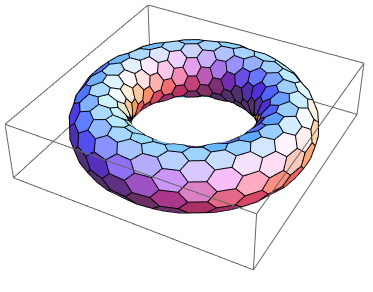
\includegraphics[width=0.75\textwidth]{images/test_image}
	\caption{H-Mode Confinement Time Scaling} ~\\
	\small This plot shows how well the ELMy H-Mode Scaling Law does for fitting $\tau_E$ to the ITER98 database of global tokamaks. For most values, the fit is at least 80\% accurate.
	\label{fig:elmy}
\end{figure}

The use of the ELMy H-Mode scaling law also brings up another subtlety in the field. To measure the movement of energy within a plasma, scaling relations are needed that correlate to specific modes of plasma behavior -- i.e.\ ones that can robustly be found on a device by technicians. Currently, people rank H-Mode scalings over L-Mode ones (because H stands for high confinement and L stands for low). However, people often seek out other modes that can reliably be found on other machines. These go by names like: I-Mode (i.e.\ intermediate confinement), Enhanced H-Mode, and Reversed Shear modes. \cite{imode,enhanced,shear}

Without going into too much detail, these alternate modes can be extremely valuable, as they often lead to more attractive reactors (than those made under H-Mode scalings). The problem, however, is often not finding a better performing mode on a single machine, but robustly finding it on other ones. This is important, because finding a mode on multiple machines is what allows new scaling relations to be produced and refined.\footnote{ In H-Mode and L-Mode's favor, they have been found on every machine that should see them. }

\section{Pricing a Fusion Reactor}

To compare tokamaks used as fusion reactors the obvious metrics are costs. ITER -- the second most expensive experiment today (only behind the LHC) -- has a history rich in countries backing out for high price tags and rejoining only when they finally get lowered. \cite{jeff} The problem is \$20B is a lot of money and 20 years is a long time. Moreover, approximating true costs becomes even trickier when designers need to project (or neglect)  economies-of-scale for expensive components, such as the magnets and irradiated materials.

As such, this paper adopts stand-ins for the conventional capital cost and cost-per-watt metrics. This is done for simplicity, for both: modeling reasons as well as conveying the two metrics to physicists. To begin, the relevant approximation for capital cost -- how much a tokamak costs to build -- is the magnetic energy. \cite{griffiths}
\begin{equation}
	W_M \propto R^3 B^2
	\label{eq:w_m}
\end{equation}
\myequations{Magnetic Energy -- $W_M$}

In this magnetic energy proportion relation, the tokamak's major radius -- R -- is involved in a volumetric term ($R^3$) and B is the strength (in Teslas) of the hooped shape magnetic field that lays nested within the plasma's shell (near its core). This quantity simply states that the two surefire ways to make a machine more expensive to build are: making it larger and using stronger magnets.

The next metric, the cost-per-watt, is defined by dividing the capital cost (i.e.\ the magnetic energy) by the main source of power output. This quantity measures how profitable a reactor will be once it is built. In a tokamak, the main power output is assumed to be fusion power, which relies on light elements (i.e.\ two Hydrogens) fusing into a heavier one (i.e.\ one Helium) -- hopefully releasing enough energy to offset the expense of causing it to happen in the first place. Although fusion power will not be defined till later, it does highlight the fact that this measure of cost-per-watt actually has units of time!\footnote{As energy per unit watt has units of time (i.e seconds).}

The final piece of the costing puzzle is a duty factor that levelizes the comparison of pulsed and steady-state tokamaks. As pulsed machines may be off 20\% of the time, their fusion power output should be reduced by that percentage. This is accounted for in the duty factor, which is simply the ratio of the flattop -- the time when pulsed machines are approximately held at steady-state -- to the entire length of the pulse. 

In pulsed machines, the entire pulse includes charging the inductive sources as well as flushing out the tokamak between runs. These non-flattop portions of time can last around thirty minutes (where the reactor makes no money). As steady-state machines lack these non-flattop portions, their duty factors are rightfully one. Analysis in \cref{section:pulse} and discussion with several researchers, however, show that the same will probably hold true for a pulsed reactor, too.

Summarizing, the cost-per-watt coupled with the duty factor provides an ad hoc pricing metric, $C_W$, given by:

\begin{equation}
	\tcboxmath{
	C_W = \frac{W_M}{f_{Duty} \cdot P_F}
	}
	\label{eq:c_w}
\end{equation}
\myequations{Cost per Watt -- $C_W$}

It serves as a cornerstone for comparing the entire landscape of tokamak reactors -- whether they run in pulsed or steady-state operation. Although not a true engineering cost metric (i.e.\ in dollars per watt), it does provide an obvious physics meaning. Coupled with the magnetic energy stand-in for capital cost, these two costs allow researchers to pinpoint profitable and inexpensive tokamaks within reactor space.

\section{Modeling a Fusion Reactor}

Before reactors can be costed, though, they have to be modeled. Therefore the first half of this thesis is devoted to the theory behind tokamak design. A priority is placed more on a physicist's intuition than an engineer's costing rigor. This is justified by the nonlinearities inherent to the fusion systems and rationalized by this paper's results matching more sophisticated frameworks with high fidelity.

What makes this paper's model different from others in the field is the generalized handling of both modes of tokamak operation: pulsed and steady-state. This was necessitated by a desire to compare the two modes on a level playing field. What this shows is that both pulsed and steady-state tokamaks could make for profitable fusion reactors -- assuming some technological advancements.

One technological advancement that could lead to major wins is improving magnet components. This is why MIT has championed high-field designs for the better part of the last century. In their latest effort, the PSFC team has explored new high-temperature superconducting (HTS) tape capable of doubling the maximum achievable field strength. What this paper shows is that this logic is indeed correct and that HTS tape is all that is needed to build optimum reactors.

More concretely, this paper shows that new HTS tape technology is capable of lowering both pulsed and steady-state tokamak costs. Further, the benefits of doubling the magnet strength bring the situation to a realm of significantly diminished rates of return. HTS is thus the end goal for the conventional D-T fusion paradigm. 

Moreover, this model shows that HTS is best utilized in different components for pulsed and steady-state operation. Steady-state tokamaks favor HTS use in the D-shaped magnets that circle the machine (i.e.\ the TF coils). Whereas pulsed devices would benefit from employing HTS in the central solenoid -- that produces most of a reactor's inductive current. A corollary of this is \replaced{the more conventional low-temperature superconducting (LTS) magnets (i.e.\ less expensive ones)}{conventional copper magnets (i.e.\ inexpensive ones)} can be used for pulsed TF coils, as their improved confinement saturates at much lower field strengths.

Now that the problem has been thoroughly introduced, we will go over the theory behind steady-state and, then, pulsed tokamaks. A couple segues will be taken along the way to show how the model can be incorporated into a fusion systems code. This code -- Fussy.jl -- is the topic of an appendix chapter and is freely available at:
 
{\centering \href{http://git.io/tokamak}{git.io/tokamak} \par }

\clearpage

\newpage

\begin{figure*}
    \centering
    \hfill 
    \begin{subfigure}[t]{0.42\textwidth}
        \centering
    \begin{adjustbox}{width=\textwidth}
      \Large
      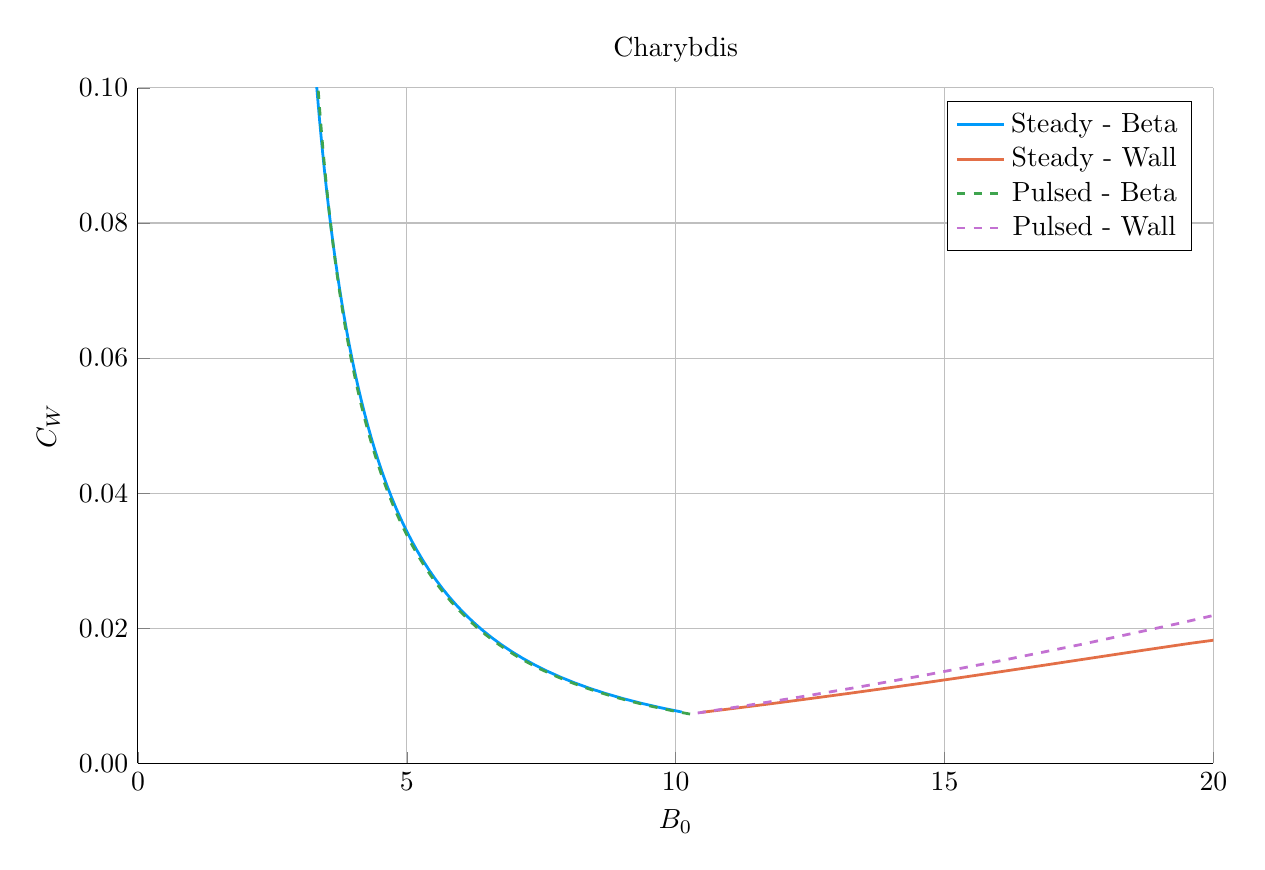
\begin{tikzpicture}[]
\begin{axis}[height = {101.6mm}, ylabel = {${C}_{W}$}, title = {Charybdis}, xmin = {0.0}, xmax = {20.0}, ymax = {0.1}, xlabel = {${B}_{0}$}, {unbounded coords=jump, scaled x ticks = false, xticklabel style={rotate = 0}, xmajorgrids = true, xtick = {0.0,5.0,10.0,15.0,20.0}, xticklabels = {0,5,10,15,20}, xtick align = inside, axis lines* = left, scaled y ticks = false, yticklabel style={rotate = 0}, ymajorgrids = true, ytick = {0.0,0.02,0.04,0.06,0.08,0.1}, yticklabels = {0.00,0.02,0.04,0.06,0.08,0.10}, ytick align = inside, axis lines* = left,     xshift = 0.0mm,
    yshift = 0.0mm,
    axis background/.style={fill={rgb,1:red,1.00000000;green,1.00000000;blue,1.00000000}}
, colorbar style={title=}}, ymin = {0.0}, width = {152.4mm}]\addplot+ [color = {rgb,1:red,0.00000000;green,0.60560316;blue,0.97868012},
draw opacity=1.0,
line width=1,
solid,mark = none,
mark size = 2.0,
mark options = {
    color = {rgb,1:red,0.00000000;green,0.00000000;blue,0.00000000}, draw opacity = 1.0,
    fill = {rgb,1:red,0.00000000;green,0.60560316;blue,0.97868012}, fill opacity = 1.0,
    line width = 1,
    rotate = 0,
    solid
}]coordinates {
(10.112818033153026, 0.007598383414978856)
(9.722156888543116, 0.008230424223188452)
(9.357875603858393, 0.008896404207575682)
(9.017653755630063, 0.009597023567402527)
(8.6995124437054, 0.010332804662622194)
(8.401566530516865, 0.011104394978990672)
(8.122163706328223, 0.011912345200844093)
(7.859819415455661, 0.012757161102175962)
(7.613196557650265, 0.013639302343912054)
(7.381088038653343, 0.014559181429827196)
(7.162401716104116, 0.015517162820285028)
(6.956147367527331, 0.016513562202290014)
(6.761425371986388, 0.017548645913683623)
(6.577416849463348, 0.018622630518712633)
(6.403375044688587, 0.019735682531644493)
(6.2386177769852695, 0.02088791828458706)
(6.0825208065966905, 0.022079403933712667)
(5.934511989185341, 0.02331015560822712)
(5.794066116682695, 0.024580139674436858)
(5.660700347012839, 0.02588927313954039)
(5.533970150598111, 0.027237424167073223)
(5.413465705416883, 0.02862441270831249)
(5.298808685607224, 0.03005001123436344)
(5.189649392059402, 0.031513945582432444)
(5.085664187259174, 0.033015895883282464)
(4.986553195072601, 0.03455549758379169)
(4.892038235455667, 0.03613234255000151)
(4.801860966679364, 0.037745980245626594)
(4.7157812114040425, 0.03939591897965519)
(4.633575445956479, 0.041081627216715676)
(4.5550354347559185, 0.04280253494397791)
(4.479966994069385, 0.04455803508845128)
(4.408188871204256, 0.046347484978679)
(4.33953172691477, 0.048170207844964834)
(4.273837210246432, 0.05002549435242988)
(4.210957116299974, 0.051912604161371986)
(4.15075261849161, 0.053830767509593334)
(4.0930935678432965, 0.05577918681155204)
(4.037857852672517, 0.05775703826940529)
(3.9849308127842145, 0.05976347349121981)
(3.9342047029103653, 0.06179762111185749)
(3.8855782007091695, 0.06385858841225403)
(3.838955955133626, 0.06594546293303978)
(3.7942481714200484, 0.06805731407868133)
(3.7513702293348077, 0.07019319470855978)
(3.710242331663442, 0.07235214271160313)
(3.6707891802306123, 0.0745331825613442)
(3.6329396770109583, 0.07673532684849063)
(3.5966266481325166, 0.07895757778829673)
(3.5617865887889004, 0.08119892870027327)
(3.5283594272686503, 0.08345836545794902)
(3.496288306480746, 0.08573486790664452)
(3.465519381509793, 0.08802741124736263)
(3.4360016318699595, 0.09033496738515884)
(3.4076866872513096, 0.0926565062404898)
(3.380528665662031, 0.09499099702224018)
(3.3544840229690007, 0.09733740946131986)
(3.3295114129297314, 0.09969471500383864)
(3.3055715568879336, 0.10206188796308927)
(3.2826271223788512, 0.10443790662966322)
(3.260642607548369, 0.10682175444066445)
(3.239584247604666, 0.10921242049746493)
(3.2194198921826622, 0.11160890156230109)
(3.2001189373344725, 0.11401020198268878)
(3.181652227422265, 0.11641533509457672)
(3.163991977015565, 0.11882332397376366)
(3.1471116955378684, 0.12123320224599504)
(3.130986116696265, 0.12364401485456963)
(3.115591132350856, 0.1260548187858383)
(3.1009037305081053, 0.12846468375306214)
(3.0869019371473265, 0.13087269283917113)
(3.0735647616124355, 0.13327794309901428)
(3.0608721453218655, 0.13567954612178545)
};
\addlegendentry{Steady - Beta}
\addplot+ [color = {rgb,1:red,0.88887350;green,0.43564919;blue,0.27812294},
draw opacity=1.0,
line width=1,
solid,mark = none,
mark size = 2.0,
mark options = {
    color = {rgb,1:red,0.00000000;green,0.00000000;blue,0.00000000}, draw opacity = 1.0,
    fill = {rgb,1:red,0.88887350;green,0.43564919;blue,0.27812294}, fill opacity = 1.0,
    line width = 1,
    rotate = 0,
    solid
}]coordinates {
(20.758867641064707, 0.018765308409143346)
(20.346250098246923, 0.018594952760163406)
(19.57104597888471, 0.01777146918538113)
(18.681781921115476, 0.016727851446155666)
(17.775790175980152, 0.015638576778075435)
(16.896654716492492, 0.014581653280825104)
(16.063927450323227, 0.013591211730165224)
(15.285557510665852, 0.012680275903338053)
(14.563500533069154, 0.01185123263968419)
(13.896568848875791, 0.01110114677254841)
(13.281970890030232, 0.010424581221258129)
(12.716170469467318, 0.009815118917575654)
(12.195372283741088, 0.00926617943914564)
(11.715794270833433, 0.008771443174384838)
(11.273815669498969, 0.008325054959037046)
(10.866051794088186, 0.007921704192505699)
(10.489365023931143, 0.007556609136513177)
};
\addlegendentry{Steady - Wall}
\addplot+ [color = {rgb,1:red,0.24222430;green,0.64327509;blue,0.30444865},
draw opacity=1.0,
line width=1,
dashed,mark = none,
mark size = 2.0,
mark options = {
    color = {rgb,1:red,0.00000000;green,0.00000000;blue,0.00000000}, draw opacity = 1.0,
    fill = {rgb,1:red,0.24222430;green,0.64327509;blue,0.30444865}, fill opacity = 1.0,
    line width = 1,
    rotate = 0,
    solid
}]coordinates {
(10.26788634689966, 0.007291637162809203)
(9.953967652326213, 0.007763018579561715)
(9.567926244368271, 0.008410560830066265)
(9.207974394987358, 0.009093056690349528)
(8.871841888699304, 0.009811202030777346)
(8.557505525932248, 0.010565644256199823)
(8.263156925406376, 0.01135697964954635)
(7.9871752024348766, 0.01218575089778548)
(7.728103682045175, 0.013052444820635726)
(7.484629973620137, 0.01395749030938975)
(7.255568856523303, 0.014901256485610468)
(7.039847526735421, 0.015884051087442074)
(6.836492834698909, 0.01690611908975986)
(6.644620209081183, 0.01796764156282338)
(6.463424013335149, 0.01906873477252413)
(6.2921691243175495, 0.020209449523749864)
(6.13018355681404, 0.02138977074682875)
(5.97685198655569, 0.022609617323612653)
(5.831610044919842, 0.023868842161338135)
(5.693939286027163, 0.025167232481888336)
(5.563362729090489, 0.026504510357656302)
(5.439440906144732, 0.0278803334592314)
(5.321768347746793, 0.02929429601917866)
(5.209970453003084, 0.030745929990983068)
(5.103700692769835, 0.03223470641747899)
(5.002638109938164, 0.03376003696406285)
(4.906485077678376, 0.03532127563010485)
(4.814965286571576, 0.03691772061565451)
(4.727821933804548, 0.03854861633202897)
(4.644816091323922, 0.04021315554278132)
(4.565725232806084, 0.04191048162126061)
(4.490341901840154, 0.04363969091085349)
(4.418472505906755, 0.04539983517396531)
(4.349936222622964, 0.047189924115870814)
(4.284564006352339, 0.049008927969770806)
(4.222197684694192, 0.05085578012965056)
(4.162689135592264, 0.05272937981792158)
(4.105899536872315, 0.05462859477526984)
(4.051698680949713, 0.056552263960658246)
(3.9999643482627323, 0.058499200250012214)
(3.9505817337017928, 0.06046819312273483)
(3.903442920928527, 0.062458011325916454)
(3.858446400032002, 0.06446740550676137)
(3.8154966244515616, 0.06649511080452623)
(3.7745036035252744, 0.06853984939399767)
(3.7353825273991994, 0.07060033297331114)
(3.6980534213689746, 0.07267526518964869)
(3.6624408270205375, 0.07476334399712868)
(3.62847350780097, 0.07686326394192533)
(3.5960841768845415, 0.07897371837037194)
(3.565209245407392, 0.08109340155652811)
(3.5357885893311605, 0.0832210107463015)
(3.5077653333614305, 0.08535524811591486)
(3.4810856504959875, 0.08749482264305544)
(3.4556985759109375, 0.08963845188964095)
(3.4315558340122845, 0.09178486369563649)
(3.408611677587535, 0.09393279778385825)
(3.3868227380888998, 0.09608100727612065)
(3.36614788616562, 0.09822826012150637)
(3.3465481016421226, 0.10037334043786662)
(3.327986352208224, 0.1025150497680155)
(3.3104274769652595, 0.10465220838353721)
(3.2938380965241474, 0.1067836557197021)
(3.278186482171801, 0.10890825269906537)
(3.263442495132517, 0.11102488135374605)
(3.2495774839156075, 0.1131324463411963)
(3.236564206241785, 0.11522987560063444)
(3.224376752844934, 0.11731612107126856)
(3.212990475972638, 0.11939015934381376)
(3.2023819222517877, 0.12145099224802183)
(3.192528769611062, 0.12349764737898258)
(3.1834097679780142, 0.1255291785649034)
(3.1750046834890777, 0.12754466627907632)
(3.1672942459724482, 0.12954321799866983)
};
\addlegendentry{Pulsed - Beta}
\addplot+ [color = {rgb,1:red,0.76444018;green,0.44411178;blue,0.82429754},
draw opacity=1.0,
line width=1,
dashed,mark = none,
mark size = 2.0,
mark options = {
    color = {rgb,1:red,0.00000000;green,0.00000000;blue,0.00000000}, draw opacity = 1.0,
    fill = {rgb,1:red,0.76444018;green,0.44411178;blue,0.82429754}, fill opacity = 1.0,
    line width = 1,
    rotate = 0,
    solid
}]coordinates {
(48.990476413653056, 0.09724163307501366)
(42.83950920694117, 0.07766994779263652)
(37.687790427214495, 0.06269593244609177)
(33.33937742845888, 0.05109841711622891)
(29.64296398154308, 0.04201539110057761)
(26.48039367255613, 0.034828857187910324)
(23.758442882319894, 0.029089432591006322)
(21.402860298405816, 0.02446606951047545)
(19.353987387634486, 0.020711961258999954)
(17.563502020363714, 0.017641064746807725)
(15.991970371213752, 0.015111701839397276)
(14.606987499719377, 0.013014953187280779)
(13.381751501116137, 0.011266342778060628)
(12.293960329570087, 0.009799811915435606)
(11.32495111804522, 0.00856330563618739)
(10.459023415380802, 0.007515507834648486)
(10.26788634689966, 0.007291637162809203)
};
\addlegendentry{Pulsed - Wall}
\end{axis}

\end{tikzpicture}

    \end{adjustbox}
        \caption{Toroidal Field Sensitivity}
    \end{subfigure}
    \hfill
    \begin{subfigure}[t]{0.48\textwidth}
        \centering
    \begin{adjustbox}{width=\textwidth}
      \Large
      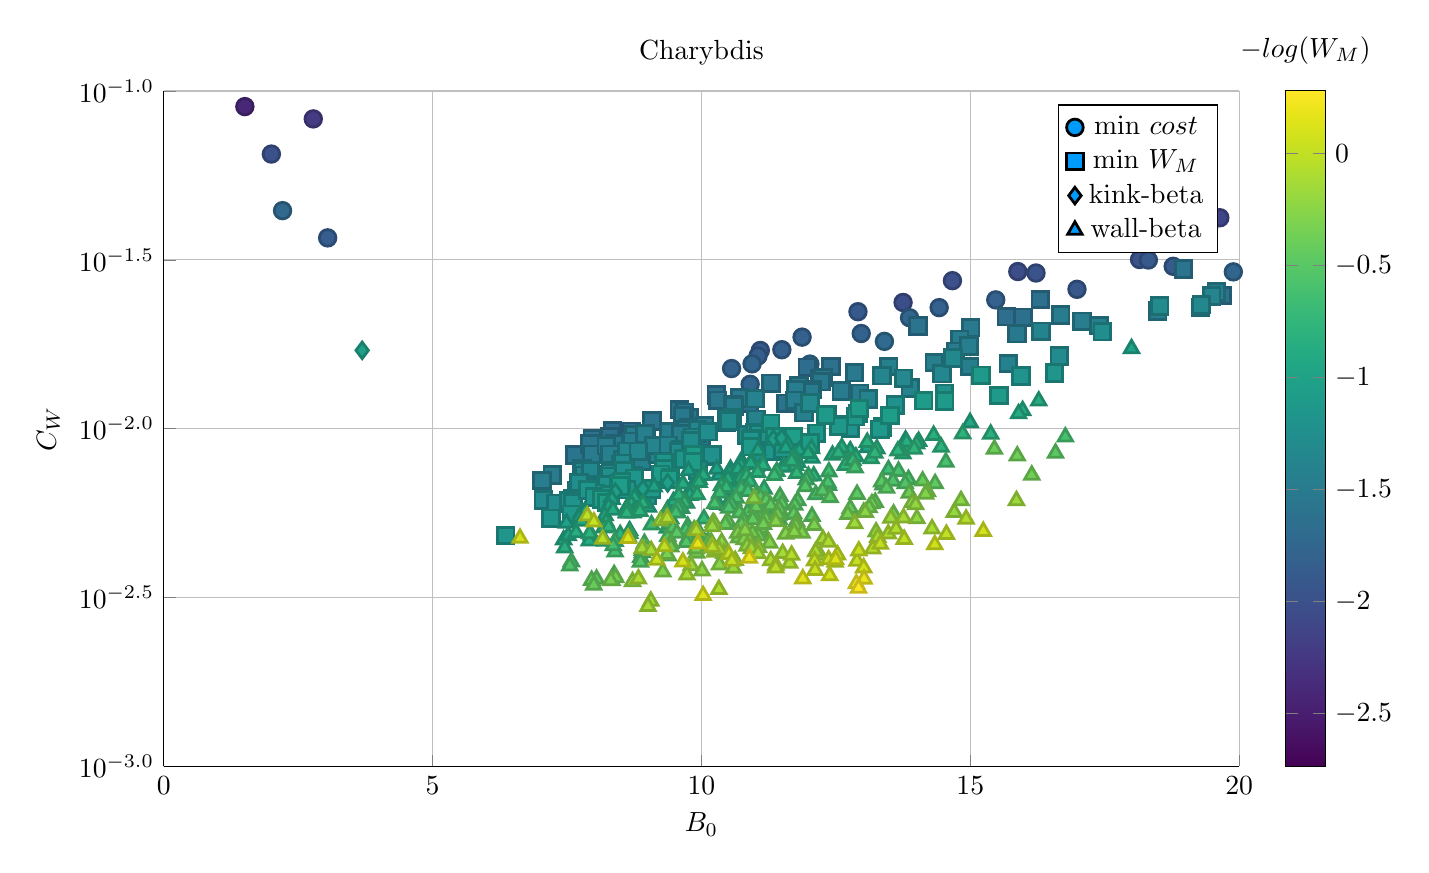
\begin{tikzpicture}[]
\begin{axis}[colorbar = {true}, height = {101.6mm}, ylabel = {${C}_{W}$}, title = {Charybdis}, xmin = {0.0}, xmax = {20.0}, ymax = {0.1}, ymode = {log}, xlabel = {${B}_{0}$}, {unbounded coords=jump, scaled x ticks = false, xticklabel style={rotate = 0}, xmajorgrids = true, xtick = {0.0,5.0,10.0,15.0,20.0}, xticklabels = {0,5,10,15,20}, xtick align = inside, axis lines* = left, scaled y ticks = false, yticklabel style={rotate = 0}, log basis y=10, ymajorgrids = true, ytick = {0.001,0.0031622776601683794,0.01,0.03162277660168379,0.1}, yticklabels = {$10^{-3.0}$,$10^{-2.5}$,$10^{-2.0}$,$10^{-1.5}$,$10^{-1.0}$}, ytick align = inside, axis lines* = left,     xshift = 0.0mm,
    yshift = 0.0mm,
    axis background/.style={fill={rgb,1:red,1.00000000;green,1.00000000;blue,1.00000000}}
, colormap={plots}{rgb=(0.26700400,0.00487400,0.32941500), rgb=(0.27794100,0.05632400,0.38119100), rgb=(0.28291000,0.10539300,0.42690200), rgb=(0.28229000,0.14591200,0.46151000), rgb=(0.27619400,0.19007400,0.49300100), rgb=(0.26514500,0.23295600,0.51659900), rgb=(0.25042500,0.27429000,0.53310300), rgb=(0.23360300,0.31382800,0.54391400), rgb=(0.21813000,0.34743200,0.55003800), rgb=(0.20123900,0.38367000,0.55429400), rgb=(0.18555600,0.41857000,0.55675300), rgb=(0.17117600,0.45253000,0.55796500), rgb=(0.15772900,0.48593200,0.55801300), rgb=(0.14618000,0.51541300,0.55682300), rgb=(0.13374300,0.54853500,0.55354100), rgb=(0.12346300,0.58168700,0.54744500), rgb=(0.11948300,0.61481700,0.53769200), rgb=(0.12632600,0.64410700,0.52531100), rgb=(0.15014800,0.67663100,0.50658900), rgb=(0.19109000,0.70836600,0.48228400), rgb=(0.24607000,0.73891000,0.45202400), rgb=(0.31192500,0.76782200,0.41558600), rgb=(0.37777900,0.79178100,0.37793900), rgb=(0.45867400,0.81636300,0.32972700), rgb=(0.54552400,0.83803900,0.27562600), rgb=(0.63690200,0.85654200,0.21662000), rgb=(0.73088900,0.87191600,0.15602900), rgb=(0.81457600,0.88339300,0.11034700), rgb=(0.90631100,0.89485500,0.09812500), rgb=(0.99324800,0.90615700,0.14393600)}, colorbar style={title=$-log( W_M )$}}, ymin = {0.001}, width = {152.4mm}]\addplot+[scatter, scatter src=explicit, only marks = {true}, color = {rgb,1:red,0.00000000;green,0.60560316;blue,0.97868012},
draw opacity=1,
line width=0,
solid,mark = *,
mark size = 3.0,
mark options = {
    color = {rgb,1:red,0.00000000;green,0.00000000;blue,0.00000000}, draw opacity = 1.0,
    fill = {rgb,1:red,0.00000000;green,0.60560316;blue,0.97868012}, fill opacity = 1,
    line width = 1,
    rotate = 0,
    solid
}] coordinates {
(43.17364371307109, 0.20372611777337152) [-2.737608795379803]
(36.93734773821979, 0.16756698485075783) [-2.687028959846787]
(48.32519073723288, 0.20307732356386315) [-2.590964172611572]
(27.818653653131317, 0.09697011319422226) [-2.5133293798402634]
(24.031609210800628, 0.08246486806905176) [-2.5100019193902536]
(46.9757183374081, 0.19848215388453824) [-2.5025824444647777]
(45.280165981821085, 0.18469850991270712) [-2.5011605733960924]
(34.33588556676648, 0.12156262800516612) [-2.487146433631915]
(49.350050230883724, 0.19851381203738652) [-2.4809660057819647]
(47.77223182347582, 0.18516332132320687) [-2.470276837036607]
(1.509009505191671, 0.08989325143911144) [-2.4120510478783452]
(1.607785753409308, 0.11208716242840429) [-2.40064821683863]
(36.7130287359324, 0.1197463715660703) [-2.3953673323479805]
(1.8837521570225992, 0.16126185747296792) [-2.393026566903574]
(40.03911031913926, 0.12157790627296668) [-2.3890711431592075]
(29.797147437037797, 0.08892691625963052) [-2.3841714318705525]
(49.837627165397436, 0.19098420146344375) [-2.3835230043455686]
(44.09667775143585, 0.1567069747417994) [-2.381290315955617]
(40.10027193508949, 0.12013460973440174) [-2.372431680776573]
(49.50704240080035, 0.18909730733563926) [-2.3528250340145016]
(28.968881363864583, 0.09075329244454268) [-2.3367870360584306]
(42.98831457790196, 0.14161197175057597) [-2.321478568273318]
(20.175934198309292, 0.05204568902739023) [-2.305558880403713]
(39.444164493588694, 0.12356138844469775) [-2.304074016625784]
(18.58289304393365, 0.04451265485552352) [-2.302767677581907]
(48.357898732015734, 0.16063854506387298) [-2.296827704935537]
(37.45895333311772, 0.10163604971512134) [-2.2875898578722627]
(38.208044910992896, 0.11621384520807569) [-2.277792210835674]
(48.821328515678495, 0.1663671711858832) [-2.2429196737605452]
(44.47436973980107, 0.14065371048755002) [-2.2307023150334016]
(36.201327387935265, 0.0992781716492562) [-2.229928759421221]
(24.976048511930994, 0.06165765133592798) [-2.225497521252979]
(2.781115265361342, 0.08264995845897197) [-2.2254079847151558]
(38.524798940282565, 0.10066936171865973) [-2.2222117952587324]
(40.75335661697331, 0.11283696845057267) [-2.2164511971368666]
(31.550557574122383, 0.07858675141449649) [-2.209080463460292]
(22.187409115367732, 0.055353669168383704) [-2.209072102647127]
(30.40343222814581, 0.08246628156983182) [-2.2082284492074966]
(22.891943050812795, 0.05534045927382465) [-2.207545754633005]
(32.48318348912026, 0.0812523499942961) [-2.2073960717358423]
(20.46108539491903, 0.04959003498021099) [-2.1906798686881843]
(24.303991155057293, 0.058916370946488036) [-2.180354292184896]
(20.69670598282277, 0.04458441983079472) [-2.1445063804884623]
(23.83667769146755, 0.05969099272190574) [-2.1441459472897755]
(19.63958505006771, 0.04213154094480493) [-2.1211539010866085]
(40.900769162095195, 0.11416954810746238) [-2.118865769548717]
(21.37751157855586, 0.04953083435602705) [-2.0989534800462293]
(33.36930679768429, 0.08867461574773429) [-2.098220502653117]
(24.013965403457117, 0.0528553369774306) [-2.0935531757786148]
(22.393434928615605, 0.05131047258257683) [-2.0908793980048204]
(29.571629059289982, 0.06966107994211436) [-2.071206080374841]
(20.977574074646927, 0.03996425224364798) [-2.064010547202469]
(18.060179054192336, 0.03708750697043753) [-2.056677518407323]
(35.94446843645834, 0.08410248770893317) [-2.046651526754166]
(15.882761260039363, 0.029196081498388402) [-2.0379011758864283]
(30.46355269165919, 0.07740613615195041) [-2.0346098603711273]
(13.74929111510663, 0.023645385119135078) [-2.0286798881208097]
(14.667163745602908, 0.027435451545116674) [-2.0136110022221563]
(40.970645504124256, 0.11225395679162868) [-2.009422091461703]
(18.86549676786543, 0.038038514881495206) [-2.0046094254929896]
(2.0018449519379766, 0.06504727548043324) [-1.9998626026906214]
(1.333016896105282, 0.1292818470624988) [-1.994011891463306]
(16.221280003397087, 0.028908830411030862) [-1.9684875514336135]
(18.146839242470875, 0.031694615819844695) [-1.962505769886516]
(20.536616448979608, 0.041976164443053174) [-1.9620022465602456]
(26.5908410355429, 0.0558374666834525) [-1.9556964151982232]
(24.564582250767256, 0.051180643617204404) [-1.951439472922028]
(19.431812066409112, 0.03938689654476367) [-1.9407104232831573]
(26.69111333219166, 0.05202238389928039) [-1.9285131737739916]
(16.98328208989546, 0.025864965787053298) [-1.9158089273231942]
(18.310414889815103, 0.0315876708787529) [-1.9026235632381945]
(23.297584692796203, 0.04007799426592172) [-1.8998797107494547]
(31.023963052023834, 0.06078277028813781) [-1.899469008660825]
(12.910038525246692, 0.022206649532263138) [-1.8922403969034376]
(41.62061738174131, 0.10343738795419383) [-1.8906275193753241]
(20.52842536101005, 0.03865878413437627) [-1.888904730447693]
(11.094220133483955, 0.01704724215883986) [-1.881726038777211]
(26.82066656529518, 0.05468787224768575) [-1.8763775212700056]
(35.10552519829791, 0.06894730353059726) [-1.8735628617782005]
(18.772509744848122, 0.030255781340376833) [-1.8728583861908288]
(27.360822192582077, 0.05616340524751281) [-1.8726476950037667]
(24.81797703498571, 0.04508699905590542) [-1.8707673950160981]
(3.0483538111563147, 0.036730885786441146) [-1.8559040168248113]
(29.522060018630928, 0.06072120698828991) [-1.844735439552174]
(39.46604489934323, 0.0887876180917983) [-1.8430067319432535]
(36.423170296938046, 0.06618962633184258) [-1.8418706711323614]
(11.051798631687303, 0.016421469596061083) [-1.839654971931263]
(25.458813886025002, 0.041749778425302704) [-1.8363695553529753]
(11.495131548398012, 0.017133631996777206) [-1.8261042714032643]
(32.71889711711922, 0.06559232169922954) [-1.8156007183182272]
(27.372160767771714, 0.050477285906930965) [-1.814915147975814]
(25.58270520703581, 0.0463768454249938) [-1.8142470512570916]
(14.420380568742246, 0.022826470712123872) [-1.8122133933822206]
(11.871194516454642, 0.018671308945999422) [-1.8120480447424478]
(15.472612894867664, 0.02406843511337114) [-1.810457309558868]
(20.542658667696518, 0.03627504764978015) [-1.8068853182048894]
(12.97099575986033, 0.019138039216325595) [-1.8019457667366159]
(21.252479627137433, 0.03724912279904193) [-1.7968505393892884]
(10.560232043643675, 0.015068032824050809) [-1.7952329403066731]
(45.12856703204009, 0.10460346899306477) [-1.7847262081815998]
(42.21258282310005, 0.09611727933154134) [-1.7840094275762153]
(13.869520871341438, 0.021310065419317785) [-1.76773605949338]
(19.89092632819806, 0.02913495659310822) [-1.7643358761825505]
(10.905382526033923, 0.013537430460188857) [-1.7636964772599824]
(10.941389456318912, 0.015563838196545969) [-1.7631697711543228]
(22.454106310710905, 0.039135813481222324) [-1.7625125196445544]
(30.835040451521607, 0.058991966200443106) [-1.7573515468471756]
(2.20974763812607, 0.04422563848495237) [-1.7287980416000448]
(38.02614384410885, 0.07767888704178068) [-1.7234251960549989]
(32.76556364087757, 0.06204137364185275) [-1.706346162862732]
(13.40240917641803, 0.018138423087163798) [-1.7045486732225623]
(46.55916074836906, 0.09124971330207729) [-1.7014359592573747]
(22.042270993490888, 0.0365316783828158) [-1.6927990438723723]
(12.016385149605648, 0.015536674756802697) [-1.6898457437353114]
(24.29682482728058, 0.04003550886686569) [-1.6732846842044926]
};
\addlegendentry{min $cost$}
\addlegendentry{min $W_M$}
\addlegendentry{kink-beta}
\addlegendentry{wall-beta}
\addplot+[scatter, scatter src=explicit, only marks = {true}, color = {rgb,1:red,0.00000000;green,0.60560316;blue,0.97868012},
draw opacity=1,
line width=0,
solid,mark = square*,
mark size = 3.0,
mark options = {
    color = {rgb,1:red,0.00000000;green,0.00000000;blue,0.00000000}, draw opacity = 1.0,
    fill = {rgb,1:red,0.00000000;green,0.60560316;blue,0.97868012}, fill opacity = 1,
    line width = 1,
    rotate = 0,
    solid
}] coordinates {
(11.967738248169791, 0.015197399614753464) [-1.6681264025020264]
(8.696464418773537, 0.009823451646161325) [-1.663027891651841]
(8.345089297998298, 0.009846202245989184) [-1.6574639825902946]
(10.880655338826603, 0.011920058291303071) [-1.6569597902573525]
(44.33631295480244, 0.07535163980234072) [-1.6567719329389001]
(15.669504585643491, 0.02145281320442147) [-1.6490985707391912]
(10.539028948810953, 0.010980468278747128) [-1.6422304847233504]
(16.300333423271717, 0.024120165421292625) [-1.6325751861823363]
(15.984439076117749, 0.021369208393676346) [-1.6291941426087102]
(32.92820758192895, 0.059322254561326254) [-1.6271960977249518]
(12.410293143428914, 0.015274978962504819) [-1.6270750467611084]
(19.688988499386202, 0.02479273110440336) [-1.626888156587228]
(47.183683314686505, 0.08930149237460469) [-1.6249314455189936]
(8.292561647347492, 0.009464726031912818) [-1.616950986036806]
(9.588347137721799, 0.01140193486941599) [-1.6155813119347568]
(8.006641138103518, 0.008812988458667981) [-1.6136190879018757]
(39.148691259933166, 0.06439016913414505) [-1.6120765470743166]
(10.27384306214681, 0.012585512817446045) [-1.6084381516776733]
(14.028211695717372, 0.02012839274260647) [-1.6020711217447665]
(7.943473491980901, 0.008960652359910951) [-1.5956625490662]
(11.571557791481624, 0.011885919211945236) [-1.5936419030965376]
(21.806471384188846, 0.03445722055743375) [-1.591719437101271]
(7.968648039596557, 0.00935259758229712) [-1.5882416690043395]
(8.97123185854356, 0.00941739351173858) [-1.587943800614445]
(7.642159237594249, 0.008359730036220061) [-1.5878025494857624]
(10.460983583083753, 0.010419937829338555) [-1.5868755906181577]
(18.965059522862617, 0.029697190504060857) [-1.5849823271963874]
(12.194568732238995, 0.014090253789926491) [-1.5820661333237485]
(9.813866298873991, 0.009872769680224545) [-1.571414774494934]
(24.25469890895016, 0.036055486397936085) [-1.561587842338199]
(8.517935684154212, 0.009008401602884603) [-1.5604752308741954]
(9.080862100268657, 0.010548811329102839) [-1.560024208321792]
(9.789660341943907, 0.00975086483062938) [-1.5595172183929409]
(8.133164457566973, 0.008877515881031174) [-1.5547403592804268]
(10.297704899446542, 0.012128004524771618) [-1.5525172912757694]
(9.766479902832291, 0.01075120106159998) [-1.550211325130473]
(12.2632951302657, 0.01417054313300387) [-1.5499921130488996]
(11.291662119925611, 0.013636547782905628) [-1.5488389310082484]
(9.686757381363082, 0.01118682853182229) [-1.548636584215126]
(7.924713370279235, 0.009004515948176011) [-1.5484303677563682]
(8.54226502879131, 0.008589361734950092) [-1.5300696832010154]
(9.64758141032686, 0.010918478084483) [-1.5240418415006989]
(12.21993539420707, 0.013786535741271849) [-1.52035115860342]
(15.867234965970042, 0.019102159289939535) [-1.5187095286365286]
(15.007125908258939, 0.019900882686515825) [-1.5152558703618486]
(10.70858947114034, 0.01233142370653334) [-1.5130633149050525]
(8.529805552034778, 0.008998649144966384) [-1.5127417843169062]
(8.377294862413901, 0.009033035828776036) [-1.512065872282441]
(12.846715954681153, 0.014648425212785676) [-1.508698938344436]
(16.682126583618288, 0.021717369003602268) [-1.5042599211378067]
(10.58390997110411, 0.011787983533386965) [-1.5034350531454859]
(11.810966417691285, 0.013402736400337721) [-1.50170709764633]
(7.965952597674263, 0.008403497514698337) [-1.501622468932281]
(12.052123659751864, 0.013038942564365743) [-1.5014482706318735]
(14.803678461986678, 0.018390392389316428) [-1.4999954524234758]
(14.727306928855038, 0.01694354359189593) [-1.4973617780251773]
(10.061864920509048, 0.010183371556613061) [-1.497105465512374]
(40.24136746900709, 0.062282935043912684) [-1.4929511344473714]
(41.49663881325739, 0.06324187033686292) [-1.4921349419619385]
(11.804455973082419, 0.012548762978995496) [-1.4884591559674822]
(12.029939715648373, 0.012867101009559307) [-1.487363796795517]
(12.601637635718813, 0.012921001622500157) [-1.4866917975345906]
(9.754197703405268, 0.010047951074758055) [-1.4840978906845892]
(21.882416551144317, 0.03303866433608294) [-1.4824521913249147]
(12.942504869667264, 0.012726704506142847) [-1.4821332841886103]
(7.226740691315094, 0.007290805739373347) [-1.48122389777201]
(9.72526998487911, 0.00977012454088988) [-1.4804970319589599]
(7.032760703447595, 0.007020834402326414) [-1.4800609203732897]
(8.228283040534254, 0.008910343679206711) [-1.4785263901161534]
(11.757080569358145, 0.013060328514041545) [-1.4759327339004988]
(8.742108415330497, 0.009568901799246174) [-1.4716802129865878]
(10.608355718332808, 0.011686646580567617) [-1.4714171457200942]
(10.002017917096252, 0.009432683201513142) [-1.4697490463241623]
(17.076056816605465, 0.0207896268155257) [-1.469182095495403]
(9.93096524460024, 0.00970055448692835) [-1.4669160574764228]
(9.646537177073283, 0.009906198335664992) [-1.4650279037766998]
(8.492788974520707, 0.008175296861755412) [-1.4649157170050158]
(39.01795702656691, 0.06304537805517052) [-1.4637589731711664]
(37.319780376430465, 0.058293696935902015) [-1.4637269213699509]
(18.482121616159016, 0.022332692478256824) [-1.4633431723635995]
(8.698182291263416, 0.009175072172052877) [-1.4625771233357587]
(28.127107238558466, 0.03507245292213848) [-1.4624493219359893]
(24.405556044324065, 0.0323252483349636) [-1.456137936078477]
(11.740431759483823, 0.012144991566364045) [-1.4552956920106896]
(9.39566274467647, 0.009807429458519862) [-1.4545765412204814]
(14.971887946904854, 0.017552109366812733) [-1.4536933205355047]
(8.340793691955412, 0.008376880643338882) [-1.4536264367612777]
(20.758621662871732, 0.027928446404318328) [-1.4522195766945736]
(14.989566420933915, 0.015275332383460013) [-1.4474663709891824]
(14.328449262483707, 0.015700047070746036) [-1.4473086055649607]
(9.614108815012006, 0.009670159078421467) [-1.4394573389116623]
(8.946816680478415, 0.00966580645268258) [-1.43910869750835]
(17.39032103778615, 0.02020398851625505) [-1.4359212547397637]
(8.887301811416945, 0.008025741974410725) [-1.4345455569874563]
(8.293678413022477, 0.008395971364345037) [-1.4342039611389994]
(34.870157215661116, 0.055516720625521446) [-1.431939711468657]
(9.215949656599236, 0.008564631451482608) [-1.4318393301192203]
(13.483733389139449, 0.015286328537971657) [-1.4298782830268841]
(11.909294643223976, 0.011144326549623773) [-1.4297531319990848]
(19.28479299500749, 0.022836013108600235) [-1.429493152311542]
(19.574343065749268, 0.02541733792453219) [-1.4257656907023994]
(7.775559573362513, 0.007637958943877289) [-1.4246908118870814]
(25.190615990519625, 0.032702505993041836) [-1.4223151615986427]
(15.706222639321235, 0.015605848032644089) [-1.4209285260987674]
(9.186736487920959, 0.00838874188644035) [-1.4103191250155003]
(7.810243176708771, 0.007287678962320866) [-1.409160412241362]
(10.994509564269785, 0.012263516831132143) [-1.3987487890322283]
(11.014663159593116, 0.010656632838165833) [-1.3961077718749653]
(13.882977876787413, 0.013186567390631069) [-1.39553831950318]
(9.36196654538676, 0.00805251109990194) [-1.3921916689745937]
(16.3128197434878, 0.019423304332311736) [-1.391977480132208]
(21.05130093390351, 0.025114205055596032) [-1.3910450519688433]
(21.18381811006707, 0.026458278303411537) [-1.3854794296349102]
(13.100755547904486, 0.012247975078154037) [-1.3835251244626703]
(9.120715613380417, 0.008921077760690099) [-1.3812630274600655]
(7.896894254399229, 0.007416332681742631) [-1.3791460184166777]
(9.381274310380604, 0.008932161350486465) [-1.376877777579119]
(19.488100600993267, 0.024683476432383993) [-1.375791428631395]
(10.475402655568338, 0.010670268336180793) [-1.3747828318073587]
(9.32515552589659, 0.007870433585163046) [-1.3692376523933565]
(7.9286970308329465, 0.0074378152848894735) [-1.3684330757581267]
(8.538214357510187, 0.008098566001726598) [-1.3642308788975135]
(13.354119232582212, 0.014345667909698757) [-1.3639106630352087]
(8.608422674568363, 0.008572986953587419) [-1.3552608297970883]
(9.925761115396522, 0.00992037446225701) [-1.3550143961305745]
(8.004082331921554, 0.007328347073490059) [-1.3536632792649093]
(7.802422783894211, 0.007510901593863939) [-1.3520272957429909]
(14.471041037539871, 0.014541602438699657) [-1.3510576974042412]
(7.810600769649848, 0.007284218364658594) [-1.3496042220443973]
(19.296422276685288, 0.023274179527198832) [-1.341589260669594]
(8.824939461101431, 0.008576558289309913) [-1.3400141478767358]
(8.49764138867205, 0.00783880949696723) [-1.3300314493551002]
(13.758392145064837, 0.01411038207207742) [-1.3284263237560021]
(7.937511343586117, 0.007486503783717723) [-1.3242939338468662]
(14.679707952711722, 0.016172436730796002) [-1.323178727777929]
(8.319781298347303, 0.007515284989600465) [-1.3213550729926942]
(27.500324284476235, 0.031083172357107024) [-1.3188753969554132]
(7.672777169827471, 0.006572813918743706) [-1.3138992633454782]
(34.26204390685552, 0.04309583371292883) [-1.3112533972207423]
(8.305241116382918, 0.007413444843148486) [-1.3066175516543825]
(18.522037273131268, 0.02306836377257982) [-1.3040612288627607]
(9.843274954742599, 0.00943254285754032) [-1.3038133693852783]
(12.01595379328233, 0.01190899263404481) [-1.301084703290134]
(8.530188695097733, 0.00789699984651379) [-1.3010145120900876]
(7.059381386127842, 0.006149219434619409) [-1.3000605956773916]
(16.655180883583878, 0.016437005811172183) [-1.2981699890610565]
(9.606246685298759, 0.008660055713531614) [-1.2951558801969907]
(10.571439501867458, 0.010749954823506654) [-1.29444309797184]
(7.284894188691189, 0.006015009649024556) [-1.2856101424882644]
(10.842752178226151, 0.009584357937856927) [-1.285263592011844]
(34.353143867925155, 0.04494124949431044) [-1.284383793501614]
(7.905156667937178, 0.00683431321635412) [-1.2828114288158374]
(31.635765029342274, 0.039187382342347976) [-1.2826431650359629]
(8.313601928775393, 0.007231700278305266) [-1.2824255065429995]
(9.578913894726805, 0.00853616645957665) [-1.2813323109549335]
(7.924882086401339, 0.006837657402697755) [-1.2806421539894215]
(9.808329366529762, 0.009211465915111147) [-1.2790915578265545]
(10.511748242466084, 0.010542099378207213) [-1.2707451840708122]
(23.70716861300546, 0.024447750750697092) [-1.2676539939434082]
(11.00520478529279, 0.009098409772603787) [-1.2653553126366786]
(7.876105123562427, 0.006725537497980498) [-1.264293982211982]
(17.45204956258683, 0.019363431367524053) [-1.262045130852001]
(7.719844293445014, 0.006906076996276599) [-1.2611290819783112]
(10.118399421716713, 0.009803145458874337) [-1.2555987795426622]
(7.612390232156273, 0.00619895569247597) [-1.2513270179335647]
(8.729387536492673, 0.007239853513876978) [-1.2453167838780697]
(10.961169543919764, 0.008896586162085272) [-1.2430939343579344]
(10.985358154781366, 0.009719593902466845) [-1.2381773742332136]
(10.055825077383927, 0.008270424440644015) [-1.2346782486332617]
(8.291481327682558, 0.0072241626571935376) [-1.2264046023709216]
(12.335638193913455, 0.01098843719538726) [-1.2247195887884887]
(8.246208566536797, 0.006808974225612837) [-1.2180889658059086]
(8.540264952931636, 0.006611305121542242) [-1.2173874089477876]
(8.556190004184526, 0.007501419726936573) [-1.2146247722956514]
(13.602894240173864, 0.011764386053045915) [-1.2132972156104522]
(10.195221885432844, 0.008378063320530003) [-1.2109120215395388]
(11.049738848862685, 0.008427299987451904) [-1.2084181738286368]
(14.519807280009873, 0.01273555061242485) [-1.20714909048448]
(12.595222602654314, 0.010213320377511352) [-1.2033520253557135]
(26.383495577820405, 0.032086426450625864) [-1.1973567207367808]
(12.639134913781255, 0.01024990923611188) [-1.1946911954531152]
(12.771017041564328, 0.010020735618058307) [-1.194687477055283]
(11.065493657555185, 0.009634752809511687) [-1.1937967228670217]
(15.93895045303613, 0.014319974319254046) [-1.185724861965876]
(28.62771924607459, 0.030946696104817876) [-1.1815951507377263]
(7.535456478096903, 0.006119538485938838) [-1.1806237088701466]
(7.610400378886139, 0.0060467130253046425) [-1.1800813312023146]
(9.303943294896706, 0.007952378649071718) [-1.176244530950471]
(8.033169581940832, 0.006432608194369421) [-1.1748225292203367]
(7.199323628519372, 0.005427058328431804) [-1.1721208310483742]
(8.635658099111911, 0.006744537821609478) [-1.1717373686057835]
(6.357367087501427, 0.004828891223049449) [-1.1708649361692889]
(8.68097527641003, 0.006810003648499363) [-1.1692163263768098]
(10.941107168878954, 0.009353534353065332) [-1.167353919317699]
(16.564321004099757, 0.014618785296867573) [-1.1652399164280889]
(11.54197585545895, 0.008829535690276422) [-1.162809974145342]
(8.753893841415247, 0.007136024429485349) [-1.1600693635040116]
(7.885243678455898, 0.006579111152003091) [-1.157321108695414]
(11.32266327338597, 0.008599780741533768) [-1.1572067562856314]
(10.915418141745553, 0.009251618906581017) [-1.1571634670399211]
(9.667898706541429, 0.008133610271699837) [-1.154357334346231]
(12.910014006891455, 0.011084851654264415) [-1.1506586644938104]
(11.51111009989439, 0.008713510430388705) [-1.150227655836216]
(8.60996222930752, 0.006602548762005154) [-1.1491924102402016]
(8.006315067088401, 0.006272419326365313) [-1.1477835171917188]
(9.30257761823372, 0.007620679601131938) [-1.1465058315496728]
(11.285570988608995, 0.010377192915174936) [-1.145014274974487]
(12.138687953769608, 0.009696220536212618) [-1.1375870233869183]
(12.553842085049038, 0.010180634102852183) [-1.1373650551215082]
(9.934623605013899, 0.007542730978334406) [-1.1357458790371815]
(13.364635095205022, 0.010126349397671063) [-1.133986432515703]
(7.577912363275431, 0.005578205050921048) [-1.1320341014158335]
(12.86501420031779, 0.010846318354017281) [-1.127079592692178]
(8.98804676924596, 0.006331906889150134) [-1.1252988863479554]
(8.452377355502822, 0.006879141460401252) [-1.123003263844327]
(23.025824780010147, 0.022040928898795047) [-1.1207682191899027]
(13.322832437569058, 0.00996173564893061) [-1.1180749050851169]
(9.076598934998714, 0.006626896988025552) [-1.1159299024060154]
(15.198462033251472, 0.014399132022875615) [-1.111366047368976]
(14.521859369334845, 0.01206983625295502) [-1.1093461418096882]
(8.297041065786505, 0.006356432017833017) [-1.1083223146390213]
(15.534651072689927, 0.012535144034281957) [-1.108020004377878]
(10.912955767488512, 0.00883860338226376) [-1.1055395253528022]
(12.308396510673756, 0.010954609847675004) [-1.1018087579792433]
(8.515520072517582, 0.006955673427821012) [-1.1000312304906807]
(12.935222387807004, 0.011476323196829152) [-1.0958683903566835]
(14.133023152666118, 0.012099180088161502) [-1.0918611830445206]
(9.240930260616448, 0.007324655445979312) [-1.084008635561983]
(9.850752183763255, 0.008347799057721199) [-1.0818442729737123]
(9.835917844908545, 0.007973263522900845) [-1.0762205003226006]
(13.503659427877482, 0.010946001598484297) [-1.0742112770850791]
(12.015541559387604, 0.009087852412631436) [-1.0708769548182164]
(8.48180872327906, 0.0067597442860644836) [-1.069695292943837]
(9.426016311012596, 0.007160447099405331) [-1.0603710996179994]
(11.370815749528317, 0.009473258949863166) [-1.058639833713732]
(8.145331814193963, 0.0061899243692649306) [-1.0559914680496412]
(11.710887773696074, 0.009482529791919412) [-1.0537452246128203]
(9.401232433154894, 0.00708059455566661) [-1.0532767994986825]
(8.244715434296548, 0.006035560775312132) [-1.0518252532905286]
};
\addlegendentry{min $cost$}
\addlegendentry{min $W_M$}
\addlegendentry{kink-beta}
\addlegendentry{wall-beta}
\addplot+[scatter, scatter src=explicit, only marks = {true}, color = {rgb,1:red,0.00000000;green,0.60560316;blue,0.97868012},
draw opacity=1,
line width=0,
solid,mark = diamond*,
mark size = 3.0,
mark options = {
    color = {rgb,1:red,0.00000000;green,0.00000000;blue,0.00000000}, draw opacity = 1.0,
    fill = {rgb,1:red,0.00000000;green,0.60560316;blue,0.97868012}, fill opacity = 1,
    line width = 1,
    rotate = 0,
    solid
}] coordinates {
(8.305244154675892, 0.006083501631057066) [-1.0496814932160978]
(8.913067820493207, 0.006629793134010975) [-1.0478282176510978]
(11.088375868477236, 0.00764908073743482) [-1.0476862508436227]
(8.893467896647309, 0.005862884354721373) [-1.0434060376287386]
(11.339319277973114, 0.009322710512378526) [-1.042586757918211]
(8.397189975968995, 0.006487752068877104) [-1.0395059774095508]
(11.489774589946819, 0.009374281366493263) [-1.037130039873791]
(3.690186058729787, 0.0170614588554745) [-1.0308313508546258]
(9.371675394558984, 0.006913114243597262) [-1.0275590312193816]
};
\addlegendentry{min $cost$}
\addlegendentry{min $W_M$}
\addlegendentry{kink-beta}
\addlegendentry{wall-beta}
\addplot+[scatter, scatter src=explicit, only marks = {true}, color = {rgb,1:red,0.00000000;green,0.60560316;blue,0.97868012},
draw opacity=1,
line width=0,
solid,mark = triangle*,
mark size = 3.0,
mark options = {
    color = {rgb,1:red,0.00000000;green,0.00000000;blue,0.00000000}, draw opacity = 1.0,
    fill = {rgb,1:red,0.00000000;green,0.60560316;blue,0.97868012}, fill opacity = 1,
    line width = 1,
    rotate = 0,
    solid
}] coordinates {
(7.490392990216207, 0.005256053052710575) [-1.025114084474608]
(10.324607857349502, 0.007284527271346537) [-1.025064662372027]
(10.786179524347823, 0.00782078493256419) [-1.0135716419780334]
(8.265254899703113, 0.005878041854646887) [-1.0133032391552028]
(9.759627120315386, 0.007516810149579491) [-1.0129395602075102]
(7.765989799277702, 0.005642606316680264) [-1.0090683465802397]
(10.284485653997232, 0.007590586049588419) [-1.00487994972194]
(10.740566234689192, 0.008018904893245096) [-1.0024486517409639]
(7.82952747253988, 0.005687012650490601) [-0.9982503197852052]
(17.997767505161434, 0.017272851302606376) [-0.9980863049007114]
(11.607406337271188, 0.008976011549139531) [-0.9976413099828907]
(9.120664508219399, 0.00672377146821775) [-0.9952427135597887]
(8.33813410692626, 0.006179152610909006) [-0.9882704184280687]
(9.809381065883368, 0.006658577387207133) [-0.9865959618907963]
(11.05015741923656, 0.008611185683760977) [-0.9861502224644026]
(11.81726987578575, 0.00861006159819778) [-0.9834884062410291]
(9.955965615750785, 0.007078972975952707) [-0.9755470230412873]
(10.468778589579204, 0.007165169234302644) [-0.9751682968759733]
(8.275975247764718, 0.00588288059860778) [-0.9745460269854277]
(11.56641933994839, 0.008762707263760248) [-0.9724510296030006]
(7.729666360230168, 0.0054508764537053) [-0.9721723790112873]
(10.728788856458863, 0.007500206088288035) [-0.9683079871351761]
(13.794818258324069, 0.00925430650881406) [-0.9640479639625688]
(10.68702976676658, 0.007713542274813112) [-0.9605456904465843]
(13.086397858972267, 0.008793232884908199) [-0.9509475064598062]
(10.540636515545728, 0.00758530046831779) [-0.9475613034981963]
(14.994597091286334, 0.010432599107525612) [-0.9431073279051986]
(10.771912405971477, 0.006669463740427501) [-0.9395228095882537]
(7.437916255626304, 0.004688262944849126) [-0.9379797386819722]
(9.01626097658872, 0.005855680709409532) [-0.936956260188316]
(7.522698377806809, 0.004823068577046762) [-0.9328401416066296]
(8.754915642687301, 0.006257853989784519) [-0.9307108052550614]
(10.594981119045784, 0.006461854726339168) [-0.9281558619803609]
(12.045885329425058, 0.008735963170322575) [-0.9264995775599043]
(7.771430799983934, 0.005328057424477724) [-0.9262426999191099]
(10.735292233144142, 0.007790932759723544) [-0.9227003718927437]
(10.512921169293449, 0.007406866683715918) [-0.9211202387251416]
(7.950782637474951, 0.004842693465206878) [-0.9122780994598872]
(8.205592174769814, 0.00553456744660005) [-0.9098639973117462]
(10.931685642752342, 0.00799774423691871) [-0.9085892171866993]
(15.972145415340275, 0.011322447729645281) [-0.9043705523492929]
(12.054696727590375, 0.008178982728725071) [-0.903352069757217]
(8.649488124233137, 0.0058981820527739225) [-0.9005612951337819]
(9.785411486209819, 0.006353815969057234) [-0.8985196847828957]
(8.355237320864756, 0.005739892493181049) [-0.8983797144291398]
(10.676348105658398, 0.007583618995886536) [-0.8971261027713628]
(9.478163505938792, 0.006081355532545074) [-0.8962149920198969]
(10.912879849760056, 0.007895141300507174) [-0.8947574466288085]
(11.983353362889243, 0.008446442250875192) [-0.8916300803179569]
(16.272383561884997, 0.012086236110976131) [-0.890947883956792]
(11.52098349265942, 0.007728598763745398) [-0.8865999168444305]
(10.536757160705346, 0.006968625853256571) [-0.8862290860463612]
(9.655565692459556, 0.00686791587727973) [-0.8853692596179883]
(15.897115425748877, 0.011077289150155845) [-0.884029767456243]
(8.695755457607955, 0.005982150284429834) [-0.8837850767800522]
(10.492158100051922, 0.007098671990886852) [-0.8828563557879437]
(10.037701951865458, 0.0072796273438267495) [-0.8804549747402444]
(11.638039502619437, 0.007792003070402551) [-0.8799662830695792]
(11.546710974717332, 0.007704064980519725) [-0.8744133357565225]
(8.726391874140708, 0.0056363780626130485) [-0.8730986298376362]
(8.663680556671139, 0.004988178616679241) [-0.8728030894608018]
(13.787374648539751, 0.008770502666972253) [-0.8727320299344076]
(12.766608989345242, 0.008601244202966506) [-0.8720334149277572]
(7.912625943172549, 0.004655770362479482) [-0.8693487943882443]
(10.513846731080314, 0.006084065906903396) [-0.8630202034214742]
(7.669338719372169, 0.004924842040843803) [-0.861299793442028]
(8.225117880579704, 0.005298172414294102) [-0.8595038240809204]
(8.203452347735475, 0.0046473625238345456) [-0.8567854750862633]
(8.606501005951438, 0.005815101976145971) [-0.8560196956809655]
(12.610505281824743, 0.008787976150626518) [-0.8549409997795642]
(8.607112161141583, 0.005657937584887749) [-0.8549130093089008]
(14.038960987293587, 0.00917703801839012) [-0.8535716907113037]
(12.43732861090992, 0.008347881751030625) [-0.8521148893133685]
(10.730288560624734, 0.007128967537191795) [-0.848258534769848]
(13.814182568957458, 0.009136355586300991) [-0.8460593767435973]
(10.614949449057972, 0.006518603909074656) [-0.8436096023361083]
(8.910346704261844, 0.006010163492689091) [-0.8427994583004987]
(11.789269747471279, 0.007945945585113466) [-0.841947416622939]
(9.721588138355992, 0.0060248058000312785) [-0.840612447094069]
(7.4570907362874745, 0.004440943928455613) [-0.840512586473128]
(11.749954066883152, 0.008192611227802852) [-0.8396933257766793]
(11.145583374518681, 0.007794162811523137) [-0.8357637262102798]
(14.002098633144497, 0.009012091589396549) [-0.8345082268411569]
(11.71396125221291, 0.008170154991858254) [-0.8326261675235949]
(9.954982275936574, 0.006937374865533122) [-0.8320882392153445]
(9.368409582792285, 0.005749714926123568) [-0.8315762378530004]
(10.476236084679716, 0.00662694635784487) [-0.8307347851507457]
(15.378598226574077, 0.009642717688792466) [-0.830544413041331]
(12.871582541696636, 0.008249655917762508) [-0.8297213382977437]
(13.261596482506313, 0.00872151277844613) [-0.8286741188165131]
(13.0829776821363, 0.009115953893059449) [-0.8267848509238259]
(14.317311822247486, 0.009559156785738465) [-0.8225460718617404]
(8.639262951926671, 0.005739050504125615) [-0.8214723162104086]
(11.749576633189198, 0.00777900336077081) [-0.8201412806434945]
(12.546153140118335, 0.008465745314703852) [-0.8151576039795889]
(8.183555235334351, 0.005082760625336129) [-0.8142249848207472]
(11.675608431762104, 0.008019437945510303) [-0.8140641213229001]
(10.313233660105723, 0.005973868428211905) [-0.8103019758142813]
(7.919842291864804, 0.0048937089468515296) [-0.8012431956657198]
(8.609864055202394, 0.005621145192877696) [-0.8003481799777136]
(9.57863964924036, 0.006353153460386551) [-0.7977579467571502]
(13.746798877450388, 0.008421833334043108) [-0.7930251215824343]
(11.044783092119218, 0.007429093264895125) [-0.7890451923079399]
(14.456103371629998, 0.008826772268823495) [-0.787865286509519]
(9.919321037115749, 0.006383916218566666) [-0.7843040366780064]
(8.854683142750217, 0.005696794743220581) [-0.7839186276792087]
(10.597279263558937, 0.006115696804857897) [-0.7832803335041352]
(9.426262484951625, 0.005413509713037376) [-0.7821184247172652]
(13.65357832167086, 0.008596617727968549) [-0.7805782205003577]
(14.85793053450062, 0.009659872283801132) [-0.7798419979328133]
(13.154203573323626, 0.008159117975808313) [-0.779526126485372]
(12.747830729091781, 0.00801636696090187) [-0.7754633993416067]
(13.223550772820014, 0.008468144805643287) [-0.7736782567370082]
(12.088805642739427, 0.007247388825611958) [-0.7730881104428101]
(8.488492913699757, 0.004861686496363432) [-0.771875090323587]
(10.495316608073319, 0.005934301325116477) [-0.7684162906476206]
(9.362567206766446, 0.005077595748671911) [-0.7679743247932476]
(10.372000769339135, 0.006786674226710283) [-0.7648185888526707]
(8.27284371455478, 0.005109733182186724) [-0.7640789887074095]
(13.955087628156079, 0.008706119585241447) [-0.761342175922955]
(10.544958602900675, 0.005941882664679825) [-0.7543127087245246]
(11.77031037870365, 0.007371584809935278) [-0.7536484511278393]
(10.836697344568485, 0.007235631321785017) [-0.7503956953450397]
(12.6755982178082, 0.007794584633403252) [-0.7487808552191573]
(12.814719377106297, 0.008059650365173391) [-0.7476061772087611]
(10.900321708767143, 0.006963610302502873) [-0.7471256555265617]
(10.461287221109892, 0.006698880656946609) [-0.7413304463691416]
(9.558670032438643, 0.005641975327508916) [-0.7367054574686347]
(9.682364623465833, 0.006032870871331476) [-0.7331219552552337]
(11.16543967690182, 0.006626912607429937) [-0.7143600945963312]
(11.401694656436039, 0.007474831733495699) [-0.7106398428950327]
(9.939172881280367, 0.0049761893476396495) [-0.6960873863412442]
(10.046704529687267, 0.005409555517719824) [-0.6958903955949629]
(11.07309218913271, 0.005844386265058715) [-0.6930492540076382]
(9.631413377269118, 0.00580869705512685) [-0.6929516890222392]
(9.0705472826982, 0.005195474212399125) [-0.6915921881710438]
(10.340119383327263, 0.006450299363758911) [-0.6857195379800745]
(11.988661863115587, 0.007235955498415392) [-0.6856480650317041]
(11.356954793810704, 0.007277002386326683) [-0.6825231692879921]
(9.559961062893178, 0.005826409813708321) [-0.6799325504597861]
(11.1835890784689, 0.005748438997690529) [-0.6756496749536086]
(8.391628360065997, 0.004642372121698665) [-0.6668421547656437]
(11.949965044033023, 0.0070613972149505) [-0.6594486343899455]
(9.397214543064022, 0.005204006670639966) [-0.6592191769587943]
(10.74094896614302, 0.006638640066368149) [-0.6536209377575128]
(13.476998824812561, 0.007561107269230883) [-0.650948550154174]
(12.36964710930465, 0.0074536379991662315) [-0.6505954513533947]
(9.341639857223466, 0.00562511440860501) [-0.649384718466127]
(9.524994554706348, 0.0056379604361593005) [-0.6434610863211887]
(8.667648129644444, 0.004893302789367808) [-0.6386314300711667]
(10.86703111417762, 0.006520915492483144) [-0.6385156325462752]
(8.903387056823963, 0.004295648023998173) [-0.6376426431852426]
(8.39310786606612, 0.0043195416112934695) [-0.63745836942971]
(8.35978027986981, 0.004504479712425151) [-0.634161727858793]
(11.107940679063978, 0.00550347046899009) [-0.6307004133850902]
(12.85647542381142, 0.0076645781815444635) [-0.6183303859395417]
(8.639519611289709, 0.004777548127961022) [-0.6130870829164431]
(9.745180550219304, 0.005139848231321853) [-0.6129648030838463]
(16.767571242014334, 0.009455939774823839) [-0.6084696230229766]
(10.246078544026743, 0.005998204689845081) [-0.6069152599086628]
(10.644474286152628, 0.006234008404953501) [-0.6054076068022625]
(10.558536641296014, 0.005960524285263344) [-0.6024296737568321]
(8.8713583098509, 0.004158248718194877) [-0.6015484963981724]
(12.361855328211519, 0.006792484353594769) [-0.6012984238357434]
(9.29332885392237, 0.0053623804243832325) [-0.5960707607608329]
(11.022485713541675, 0.006374522460113841) [-0.5936136176179417]
(14.544923574963594, 0.007967211841028115) [-0.5931302760876686]
(7.580679209591517, 0.0040369634147211595) [-0.5915885524237119]
(12.35005177039308, 0.006918880590157332) [-0.5911727158362008]
(8.939525190055026, 0.004576324737559804) [-0.5900682137185816]
(13.665039848744003, 0.0074842396419395755) [-0.5884302817228046]
(9.713564610860795, 0.005019503207090587) [-0.5877411509443977]
(12.126528919726603, 0.006377695642268969) [-0.5867809186460089]
(11.440704257189838, 0.005390939798069345) [-0.5825897309583699]
(10.508484132698012, 0.005822320038436803) [-0.5801191442990684]
(13.849878080699321, 0.007078947827278213) [-0.5723010609292049]
(9.374762480988647, 0.004797737450304729) [-0.5679221681687051]
(9.752323594641952, 0.004745752868187461) [-0.5631840336886528]
(7.551644254176505, 0.00392267122135458) [-0.5608362242209843]
(13.563019186288107, 0.0069992567132512) [-0.5571205537040459]
(10.980344118197824, 0.006126321093742513) [-0.5485242916279889]
(13.788594176245665, 0.006874419461623871) [-0.5418068538132612]
(13.375319234807094, 0.006822436837333278) [-0.5416427697741687]
(10.855430367894837, 0.005644924884791849) [-0.5402605106654789]
(11.931629567657803, 0.0067352955911504) [-0.5386131387961719]
(11.460783403825179, 0.006300681826786258) [-0.5359571495451664]
(8.900383653315783, 0.004361609192009016) [-0.535080858548875]
(9.718967895206884, 0.004607755561392721) [-0.5306887960741941]
(11.790942156263833, 0.0061242176982959935) [-0.5279445193313689]
(11.11832225535947, 0.005699821777253932) [-0.5261185431060132]
(8.375897572810382, 0.0036996967788339836) [-0.5222207530468324]
(8.865085382679942, 0.0040283964244842855) [-0.5213443855242413]
(12.252425259957667, 0.00654764695467552) [-0.5183202512122866]
(11.487278273941813, 0.005565518290350856) [-0.5127600710400247]
(11.095685417577602, 0.006257154173968822) [-0.5093311143657722]
(9.471660054644722, 0.005081917135024615) [-0.5092608114367078]
(10.70678890662084, 0.005634560391700447) [-0.5060145289105423]
(11.032486649342086, 0.005696558547132009) [-0.4991936251195474]
(13.352670922926903, 0.006963136499419175) [-0.4985513425302997]
(11.734657678462304, 0.005936448000755268) [-0.49568499824767104]
(12.055781244217124, 0.005499933154622071) [-0.49145223309081343]
(10.78233329277987, 0.005365451873400001) [-0.489720395145329]
(9.542508252809819, 0.00491035857559783) [-0.48946631183449096]
(11.05073334272965, 0.005551912726236007) [-0.4844323986419559]
(9.94400856308007, 0.004748719229574022) [-0.48348457652780674]
(16.58389735249392, 0.008465503287908559) [-0.4828289975574789]
(12.39306388158575, 0.006257332981884576) [-0.4809853618707981]
(9.379598213601293, 0.004200694755861984) [-0.4809735664575194]
(11.493178913107707, 0.0059994354167316145) [-0.4808665748655182]
(8.332702974211756, 0.003555536540962884) [-0.47941962356708046]
(13.44284602192036, 0.0066692846879273) [-0.47870566324028313]
(11.206320448126096, 0.006131865359849344) [-0.4657796688745686]
(12.893136948528893, 0.006395516513040164) [-0.46371269394589404]
(10.990275740458832, 0.005496536453572034) [-0.45939503859612524]
(10.747891384870442, 0.005214384126637902) [-0.4580684801880486]
(11.427273011202958, 0.0055399395484132434) [-0.4551930791506963]
(8.049389553757022, 0.0035852448301646562) [-0.4548470636638538]
(14.345231023152648, 0.006879940028304696) [-0.4511448351238025]
(11.287032475635504, 0.005918008902458026) [-0.4506410472161431]
(11.715912126229652, 0.005592591526077269) [-0.44462955271421334]
(11.443687641196867, 0.005788664224478401) [-0.4417671924951601]
(10.489189485475219, 0.00532175252277852) [-0.44063870628617696]
(11.015471630669209, 0.005848263216255258) [-0.437792328306716]
(10.957005752655471, 0.005381947350223633) [-0.4372128319808473]
(12.767874676809946, 0.005807357934085231) [-0.43652773545054785]
(7.958181987834607, 0.0035579027524431407) [-0.4353218816843834]
(11.387029747701952, 0.005420864551162702) [-0.43301226198144244]
(10.122157375190174, 0.004646937579329881) [-0.42496774176553237]
(13.230701978565413, 0.006054896100373839) [-0.4234566027757057]
(10.44434411883204, 0.005209006616931108) [-0.4201824434096411]
(14.112823153995304, 0.007002732156807032) [-0.41942034556894325]
(11.062061797558213, 0.0049133604129482904) [-0.41625636474955513]
(11.105456925958254, 0.004976224512696799) [-0.4153472596885677]
(7.996801458669602, 0.003443555856640112) [-0.413698533116882]
(9.426679654304635, 0.004578061980750892) [-0.40716887268106433]
(8.988447788810735, 0.004403076051908361) [-0.4054968032106688]
(11.19894911187342, 0.005401731740408723) [-0.4052996247784937]
(11.76825986958034, 0.005310951805886482) [-0.4028975857602535]
(15.44687339946091, 0.008698035154467071) [-0.39012186383455005]
(11.415852777468853, 0.005569688147985928) [-0.3893599374140784]
(13.86344621286896, 0.006443553450960519) [-0.3874731327472749]
(9.431074457481548, 0.004467008080186493) [-0.38658238651008303]
(9.952849591589269, 0.004460761734980448) [-0.3844088155607324]
(11.102745537791256, 0.005076162944946042) [-0.3841297559869705]
(11.063005437740118, 0.004818082688701254) [-0.3799233329958369]
(13.17009498491374, 0.005997359653275597) [-0.37864836021510145]
(11.797417013849147, 0.005149154541509343) [-0.36993435073896774]
(15.872912099986983, 0.008306174738593903) [-0.36922049805921237]
(11.153084760742862, 0.005209314390453537) [-0.36517136675970174]
(16.14270329821061, 0.007290638437768607) [-0.36363162472662647]
(8.403879019467869, 0.0036256611613784515) [-0.3560282417598354]
(13.115813468322328, 0.005842256453254562) [-0.3516846326479429]
(10.946014822935268, 0.004905016792320226) [-0.3492105588330574]
(13.57250123618552, 0.005590131426966687) [-0.3472840105385271]
(11.754875170811676, 0.005148015449606661) [-0.3423857768648871]
(9.908698318368758, 0.004286076178376731) [-0.34008473263330824]
(13.016952042703096, 0.0056574013522528305) [-0.33981132719586027]
(12.721738454813128, 0.005572777477606549) [-0.3368100665351775]
(9.363983047959946, 0.004245020651172842) [-0.3261286700088182]
(8.312490793858167, 0.0035524606866130194) [-0.3248828072953213]
(9.898618326327647, 0.0044119162569870325) [-0.3237537030658796]
(10.68953135457854, 0.004750368231083765) [-0.32158297109256706]
(12.098120258532854, 0.005171308764988888) [-0.31633610176099597]
(11.869585156024094, 0.004909553661940458) [-0.3101872292940103]
(10.673795467814978, 0.004909294009190796) [-0.3098160147643643]
(9.864609706286855, 0.00502576457768123) [-0.3093537996509379]
(10.13418981012766, 0.004436392853703478) [-0.3020236790754892]
(14.203404000924808, 0.006511577615926468) [-0.29745070147912883]
(10.18170663047429, 0.00461306470000636) [-0.29735951526414567]
(10.88982583318435, 0.004680465313596841) [-0.297096548566907]
(10.7931970362076, 0.004697469217442598) [-0.29644992799415604]
(9.28264959316486, 0.0037669244430361265) [-0.2938964922996455]
(11.268417417628417, 0.004587575266941993) [-0.28257092790254534]
(14.16688315629684, 0.0064078055838669235) [-0.28099252950211584]
(11.38428238816872, 0.00530715855216879) [-0.28082048228309614]
(11.56617483025201, 0.004877778130689163) [-0.27593193726701837]
(10.81286606047368, 0.0049912232219049505) [-0.2703748605364829]
(10.21521731311282, 0.005273043762881384) [-0.2690545270372634]
(11.72560521137972, 0.004937266497875911) [-0.26717424050172617]
(10.976814102447136, 0.006213446728866137) [-0.265997200376606]
(13.046910966614577, 0.0056524730424728446) [-0.25038689413733667]
(10.335584266613429, 0.003954761985215201) [-0.24780076823439073]
(10.010917187183093, 0.0037967630657851185) [-0.24432516132466198]
(14.8272563231673, 0.006126176695457683) [-0.24228545507340632]
(13.918587840487504, 0.006043677482025348) [-0.24098176705620405]
(10.376366820059857, 0.004606765283521174) [-0.23498602936303697]
(10.243937487329118, 0.005233988553759739) [-0.23384238299419924]
(10.847268506590662, 0.004493731334283636) [-0.22307147750953485]
(14.006116168862748, 0.005417738815022194) [-0.21993321473743283]
(11.062386616188476, 0.004448263928283447) [-0.2187092653207969]
(8.718626855252902, 0.003528184507838447) [-0.2182304394283714]
(13.983583910844501, 0.005959058756527068) [-0.20811612422232886]
(13.247796771542765, 0.004950566138327164) [-0.1949465367242654]
(10.202668462679265, 0.005133692047824322) [-0.1906791623947412]
(14.700206607509946, 0.005653716907312768) [-0.18810565894941653]
(10.416291129437592, 0.004274427302329817) [-0.18713071963852396]
(10.595641202823662, 0.003864016941599036) [-0.18677877294445888]
(10.929061404350323, 0.00441554608508164) [-0.17703877611975558]
(9.238505330802848, 0.005336988341345154) [-0.17123608041269103]
(9.807859890871404, 0.003933529206939484) [-0.16802217090161298]
(13.521641900778313, 0.0054347452369170315) [-0.159632078632109]
(15.85758839281872, 0.006126736142780316) [-0.1584653585633993]
(9.05794453489073, 0.0030873738272408995) [-0.15384637826205888]
(12.849263247326576, 0.005238443186491151) [-0.15261474916905785]
(8.896720166169352, 0.004417302118131127) [-0.1399740101427423]
(13.757609358606302, 0.005445321947113288) [-0.1326527268391873]
(13.278368257880445, 0.0047684556241454085) [-0.13113219309132482]
(10.242383745816138, 0.004308730820813426) [-0.1292786219162588]
(11.511187487940832, 0.004274521004327736) [-0.1287276514871562]
(12.260363730112388, 0.0047020999988556375) [-0.1277634173442259]
(12.20260905211438, 0.004231887627104429) [-0.12738968493207978]
(10.330140219273634, 0.0043748812191618065) [-0.1269755756384773]
(11.051410932591356, 0.004265235011823922) [-0.12633579891447322]
(10.62788322731973, 0.004072522986806291) [-0.12472658311146567]
(9.064829168772716, 0.0043583870179065036) [-0.12390518423353727]
(9.730250588517745, 0.003689222647756418) [-0.11839837879753673]
(9.005938874802066, 0.0029776650111935925) [-0.11670888529278417]
(14.288501931299454, 0.005053754755206823) [-0.1088797827790834]
(8.827093733836227, 0.00359222417326949) [-0.10724377834470548]
(12.123245620220903, 0.004324887110288639) [-0.1057014515796088]
(9.90273041021652, 0.004991657187472934) [-0.09762333047105631]
(11.287886989541104, 0.004066007527325285) [-0.08986115010427638]
(11.641823986429442, 0.00399810728176478) [-0.08972858144092397]
(12.361297444519732, 0.004617875020603879) [-0.08815417484720212]
(13.474131310574805, 0.004884171206849132) [-0.08799047414483956]
(9.364389506795185, 0.0054399968889194406) [-0.08650970832660004]
(10.324641673494636, 0.0033449406828065663) [-0.07833703721847408]
(13.619088757170262, 0.005044147678571036) [-0.07809781976917668]
(11.386005862720326, 0.003945875866690141) [-0.06836893206765238]
(11.676759827185505, 0.004223534548837912) [-0.06760495405668326]
(14.921488635772578, 0.005403026282163361) [-0.061661540452943434]
(13.184711110043622, 0.004408434014542463) [-0.04494064281798065]
(11.380617481180675, 0.0038724933369633707) [-0.04318904098672454]
(10.20521510391574, 0.004460267391873656) [-0.038212612054477985]
(8.16276693983027, 0.004707734601250787) [-0.03133173591244241]
(7.874858789748727, 0.005522119503805925) [-0.023022004136594866]
(13.770047231191834, 0.0047045473818455) [-0.016271910745168695]
(12.485059190740545, 0.004024540177598891) [-0.013950276486558543]
(9.312358733139153, 0.004474130911360584) [-0.0058016737384623505]
(14.55493971443871, 0.00486934716156001) [-0.00432271776304289]
(13.325023878137985, 0.0045544637197796455) [-0.0034234668049169196]
(12.530157166099249, 0.004230145080346881) [0.0008245153063078174]
(12.102667672137938, 0.004063826320255954) [0.0009736941531625351]
(10.510345994080849, 0.004242088244665306) [0.011365608602917526]
(10.565606404055988, 0.004053843666656986) [0.017217287277544974]
(12.891616622188511, 0.004053311634801778) [0.022463112293714088]
(12.363983250719919, 0.0040944555844462105) [0.024356347238311652]
(7.9988973260130205, 0.005301589093750614) [0.024444866029481902]
(9.168830441378368, 0.004081705695114133) [0.024513255745396062]
(12.113229090441378, 0.003808447532264428) [0.030693175440979267]
(12.9268379954392, 0.00434886546170174) [0.033659198538161794]
(14.338970794985244, 0.00453657251614911) [0.06978595592755837]
(13.017028802676457, 0.0038756765128374598) [0.08105387259127383]
(15.240431681685411, 0.004970147185238468) [0.0850573900693481]
(12.385828483494706, 0.003672425930249121) [0.0924093363293227]
(9.655008703897247, 0.004032921363211944) [0.0970147585653836]
(6.626382243487151, 0.004740310225079134) [0.0995058258534219]
(12.495767737733003, 0.004094436086370008) [0.12004841257485119]
(8.634007001419924, 0.004736045243736728) [0.13042403285969037]
(10.030701314412552, 0.003208919299190161) [0.13155686422561652]
(11.884801834480777, 0.0035950709225546947) [0.1464031650577429]
(9.932474072608722, 0.004559290914970883) [0.16139055314319325]
(13.023858875261855, 0.0035888572812232517) [0.19432690543735484]
(10.889767359440034, 0.004139628207801369) [0.20016528780138218]
(12.880652990819826, 0.003476959519620879) [0.22908467155128953]
(12.921153691645934, 0.003372651368355341) [0.2806695016232924]
};
\addlegendentry{min $cost$}
\addlegendentry{min $W_M$}
\addlegendentry{kink-beta}
\addlegendentry{wall-beta}
\end{axis}

\end{tikzpicture}

    \end{adjustbox}
        \caption{Toroidal Field Samplings}
    \end{subfigure}
    \hfill \hfill ~\\ ~\\ ~\\
    \caption{Steady State Magnet Components} ~\\
    \label{fig:charybdis}
\end{figure*}

\begin{figure*}
    \centering
    \hfill 
    \begin{subfigure}[t]{0.42\textwidth}
        \centering
    \begin{adjustbox}{width=\textwidth}
      \Large
      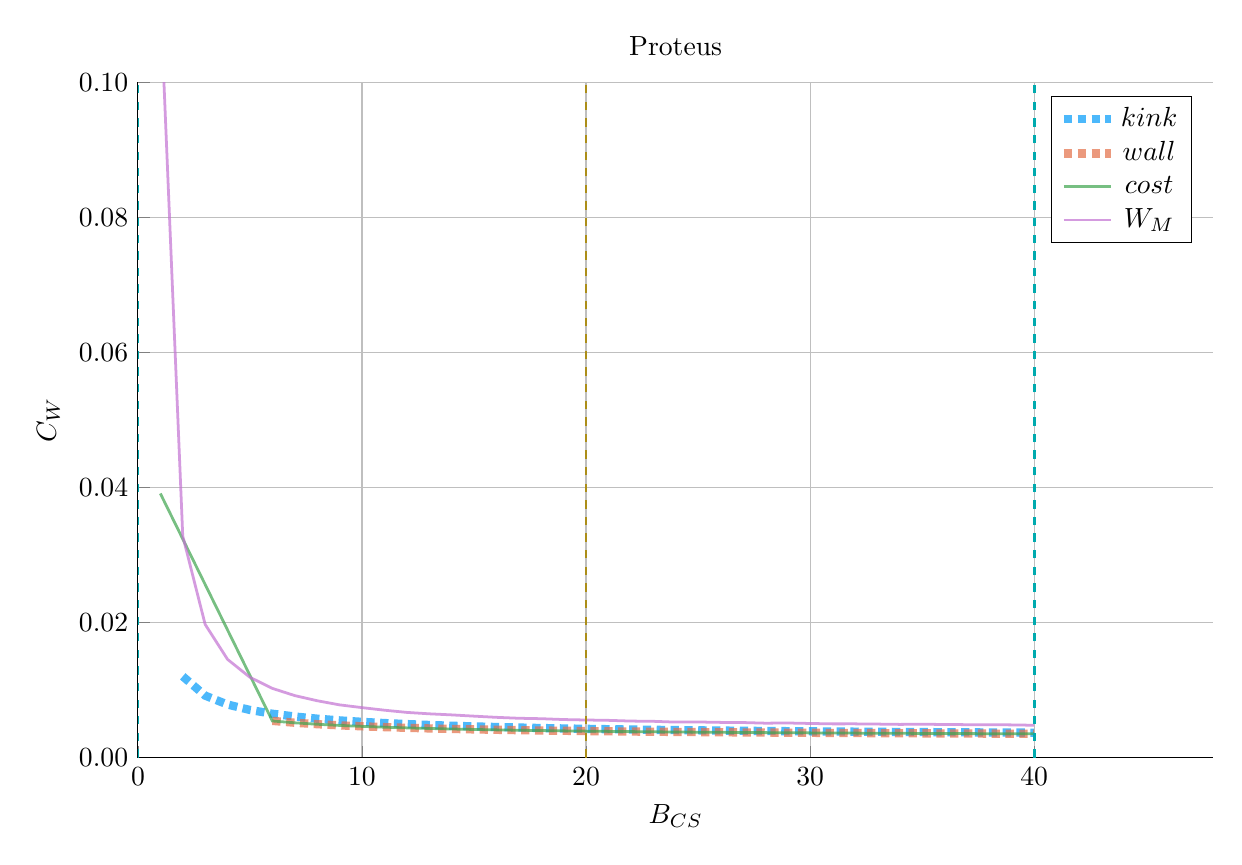
\begin{tikzpicture}[]
\begin{axis}[height = {101.6mm}, ylabel = {${C}_{W}$}, title = {Proteus}, xmin = {0.0}, xmax = {48.0}, ymax = {0.1}, xlabel = {${B}_{CS}$}, {unbounded coords=jump, scaled x ticks = false, xticklabel style={rotate = 0}, xmajorgrids = true, xtick = {0.0,10.0,20.0,30.0,40.0}, xticklabels = {0,10,20,30,40}, xtick align = inside, axis lines* = left, scaled y ticks = false, yticklabel style={rotate = 0}, ymajorgrids = true, ytick = {0.0,0.02,0.04,0.06,0.08,0.1}, yticklabels = {0.00,0.02,0.04,0.06,0.08,0.10}, ytick align = inside, axis lines* = left,     xshift = 0.0mm,
    yshift = 0.0mm,
    axis background/.style={fill={rgb,1:red,1.00000000;green,1.00000000;blue,1.00000000}}
, colorbar style={title=}}, ymin = {0.0}, width = {152.4mm}]\addplot+ [color = {rgb,1:red,0.00000000;green,0.60560316;blue,0.97868012},
draw opacity=0.7,
line width=3,
dotted,mark = none,
mark size = 2.0,
mark options = {
    color = {rgb,1:red,0.00000000;green,0.00000000;blue,0.00000000}, draw opacity = 0.7,
    fill = {rgb,1:red,0.00000000;green,0.60560316;blue,0.97868012}, fill opacity = 0.7,
    line width = 1,
    rotate = 0,
    solid
}]coordinates {
(2.0, 0.01203588028473762)
(3.0, 0.009184398565447248)
(4.0, 0.007862884013421416)
(5.0, 0.007057989599185806)
(6.0, 0.006502613319842857)
(7.0, 0.006090672614199328)
(8.0, 0.005770350019203115)
(9.0, 0.005512859892710094)
(10.0, 0.005300727695239639)
(11.0, 0.005122630604633569)
(12.0, 0.004970854616305319)
(13.0, 0.00483993073972795)
(14.0, 0.0047258536533321)
(15.0, 0.004625609812173743)
(16.0, 0.004536878856245803)
(17.0, 0.004457840030041975)
(18.0, 0.004387039347241793)
(19.0, 0.004323297793305687)
(20.0, 0.004265648725148842)
(21.0, 0.00421328852908289)
(22.0, 0.004165543387382086)
(23.0, 0.0041218418382133306)
(24.0, 0.004081697424729452)
(25.0, 0.004044691025187507)
(26.0, 0.004010460170934446)
(27.0, 0.00397868942182741)
(28.0, 0.003949102890414613)
(29.0, 0.003921458228696752)
(30.0, 0.0038955417483358588)
(31.0, 0.00387116442730114)
(32.0, 0.003848158715413871)
(33.0, 0.0038263753834889853)
(34.0, 0.003805681791784416)
(35.0, 0.0037859598267780737)
(36.0, 0.003767103936991627)
(37.0, 0.003749019788626583)
(38.0, 0.0037316235037579658)
(39.0, 0.0037148400629903496)
(40.0, 0.003698602652227772)
};
\addlegendentry{$kink$}
\addplot+ [color = {rgb,1:red,0.88887350;green,0.43564919;blue,0.27812294},
draw opacity=0.7,
line width=3,
dotted,mark = none,
mark size = 2.0,
mark options = {
    color = {rgb,1:red,0.00000000;green,0.00000000;blue,0.00000000}, draw opacity = 0.7,
    fill = {rgb,1:red,0.88887350;green,0.43564919;blue,0.27812294}, fill opacity = 0.7,
    line width = 1,
    rotate = 0,
    solid
}]coordinates {
(6.0, 0.0054444534313977866)
(7.0, 0.005168634641274746)
(8.0, 0.004954271193511655)
(9.0, 0.004781774855931542)
(10.0, 0.0046393940524333595)
(11.0, 0.004519572327657892)
(12.0, 0.004417187891782309)
(13.0, 0.004328621916738755)
(14.0, 0.004251229863078844)
(15.0, 0.004183024392188461)
(16.0, 0.004122476375660697)
(17.0, 0.004068385219748399)
(18.0, 0.004019791621043741)
(19.0, 0.003975917241919141)
(20.0, 0.003936121998618529)
(21.0, 0.0038998731854890116)
(22.0, 0.0038667227426346573)
(23.0, 0.0038362902440819057)
(24.0, 0.003808249979473852)
(25.0, 0.003782321013899768)
(26.0, 0.003758259446775421)
(27.0, 0.003735852316365348)
(28.0, 0.0037149127505960292)
(29.0, 0.0036952760721994664)
(30.0, 0.003676796641638663)
(31.0, 0.003659345275564596)
(32.0, 0.003642807117806076)
(33.0, 0.0036270798687725717)
(34.0, 0.003612072300608303)
(35.0, 0.0035977030015636596)
(36.0, 0.0035838993052924165)
(37.0, 0.003570596370170802)
(38.0, 0.0035577363809944163)
(39.0, 0.003545267851071995)
(40.0, 0.003533145007184075)
};
\addlegendentry{$wall$}
\addplot+ [color = {rgb,1:red,0.24222430;green,0.64327509;blue,0.30444865},
draw opacity=0.7,
line width=1,
solid,mark = none,
mark size = 2.0,
mark options = {
    color = {rgb,1:red,0.00000000;green,0.00000000;blue,0.00000000}, draw opacity = 0.7,
    fill = {rgb,1:red,0.24222430;green,0.64327509;blue,0.30444865}, fill opacity = 0.7,
    line width = 1,
    rotate = 0,
    solid
}]coordinates {
(1.0, 0.03911143879274214)
(6.0, 0.005431918985170686)
(7.0, 0.005156651927896806)
(8.0, 0.0049427222925668)
(9.0, 0.004770577307210836)
(10.0, 0.004628487505103093)
(11.0, 0.004508911021409933)
(12.0, 0.004406736153465557)
(13.0, 0.004318351239259131)
(14.0, 0.0042411171388798095)
(15.0, 0.004173050519899446)
(16.0, 0.00411262543808849)
(17.0, 0.0040586437812760905)
(18.0, 0.004010148222137883)
(19.0, 0.003966362101140297)
(20.0, 0.003926646631736614)
(21.0, 0.003890470261769361)
(22.0, 0.003857385855340664)
(23.0, 0.003827013846123357)
(24.0, 0.003799029152446192)
(25.0, 0.0037731515135378028)
(26.0, 0.0037491374742800476)
(27.0, 0.003726774572373303)
(28.0, 0.0037058763309042774)
(29.0, 0.0036862784148944654)
(30.0, 0.0036678355176402353)
(31.0, 0.0036504187072176437)
(32.0, 0.0036339133609214515)
(33.0, 0.003618217419267161)
(34.0, 0.003603239855200063)
(35.0, 0.0035888993956205303)
(36.0, 0.003575123536625824)
(37.0, 0.0035618476053302967)
(38.0, 0.00354901385682175)
(39.0, 0.0035365709088021192)
(40.0, 0.0035244731223137145)
};
\addlegendentry{$cost$}
\addplot+ [color = {rgb,1:red,0.76444018;green,0.44411178;blue,0.82429754},
draw opacity=0.7,
line width=1,
solid,mark = none,
mark size = 2.0,
mark options = {
    color = {rgb,1:red,0.00000000;green,0.00000000;blue,0.00000000}, draw opacity = 0.7,
    fill = {rgb,1:red,0.76444018;green,0.44411178;blue,0.82429754}, fill opacity = 0.7,
    line width = 1,
    rotate = 0,
    solid
}]coordinates {
(1.0, 0.11281791824873516)
(2.0, 0.032817502153924004)
(3.0, 0.019728226993225767)
(4.0, 0.014550673387607675)
(5.0, 0.01189537503222638)
(6.0, 0.010254586386818185)
(7.0, 0.009187722848027494)
(8.0, 0.008426409595366063)
(9.0, 0.007814460956383539)
(10.0, 0.007407116893402244)
(11.0, 0.007026609234473925)
(12.0, 0.006699623094822548)
(13.0, 0.006490049586328449)
(14.0, 0.006332285776340749)
(15.0, 0.006145121123500574)
(16.0, 0.005968637732544897)
(17.0, 0.005831116183284295)
(18.0, 0.005766436928694199)
(19.0, 0.005641758652539625)
(20.0, 0.005573536740322697)
(21.0, 0.005522757977005573)
(22.0, 0.005416005772196298)
(23.0, 0.005379655600977924)
(24.0, 0.005261536268439173)
(25.0, 0.005281022329992938)
(26.0, 0.0052218684208626695)
(27.0, 0.005199327855049588)
(28.0, 0.005104248642193906)
(29.0, 0.005130959429711627)
(30.0, 0.005061392939220031)
(31.0, 0.005001395595923804)
(32.0, 0.005003038146366862)
(33.0, 0.004969709625977857)
(34.0, 0.004924506782614121)
(35.0, 0.004946663939864212)
(36.0, 0.004912455965902953)
(37.0, 0.004883749116586274)
(38.0, 0.004871307710986148)
(39.0, 0.004851151446945242)
(40.0, 0.004795575554984452)
};
\addlegendentry{$W_M$}
\addplot+ [color = {rgb,1:red,0.67554396;green,0.55566233;blue,0.09423434},
draw opacity=1.0,
line width=1,
dashed,mark = none,
mark size = 2.0,
mark options = {
    color = {rgb,1:red,0.00000000;green,0.00000000;blue,0.00000000}, draw opacity = 1.0,
    fill = {rgb,1:red,0.67554396;green,0.55566233;blue,0.09423434}, fill opacity = 1.0,
    line width = 1,
    rotate = 0,
    solid
},forget plot]coordinates {
(20.0, 0.0)
(20.0, 0.1)
};
\addplot+ [color = {rgb,1:red,0.00000048;green,0.66575898;blue,0.68099695},
draw opacity=1.0,
line width=1,
dashed,mark = none,
mark size = 2.0,
mark options = {
    color = {rgb,1:red,0.00000000;green,0.00000000;blue,0.00000000}, draw opacity = 1.0,
    fill = {rgb,1:red,0.00000048;green,0.66575898;blue,0.68099695}, fill opacity = 1.0,
    line width = 1,
    rotate = 0,
    solid
},forget plot]coordinates {
(0.0, 0.0)
(0.0, 0.1)
};
\addplot+ [color = {rgb,1:red,0.00000048;green,0.66575898;blue,0.68099695},
draw opacity=1.0,
line width=1,
dashed,mark = none,
mark size = 2.0,
mark options = {
    color = {rgb,1:red,0.00000000;green,0.00000000;blue,0.00000000}, draw opacity = 1.0,
    fill = {rgb,1:red,0.00000048;green,0.66575898;blue,0.68099695}, fill opacity = 1.0,
    line width = 1,
    rotate = 0,
    solid
},forget plot]coordinates {
(40.0, 0.0)
(40.0, 0.1)
};
\end{axis}

\end{tikzpicture}

    \end{adjustbox}
        \caption{Solenoid Strength Sensitivity}
    \end{subfigure}
    \hfill
    \begin{subfigure}[t]{0.48\textwidth}
        \centering
    \begin{adjustbox}{width=\textwidth}
      \Large
      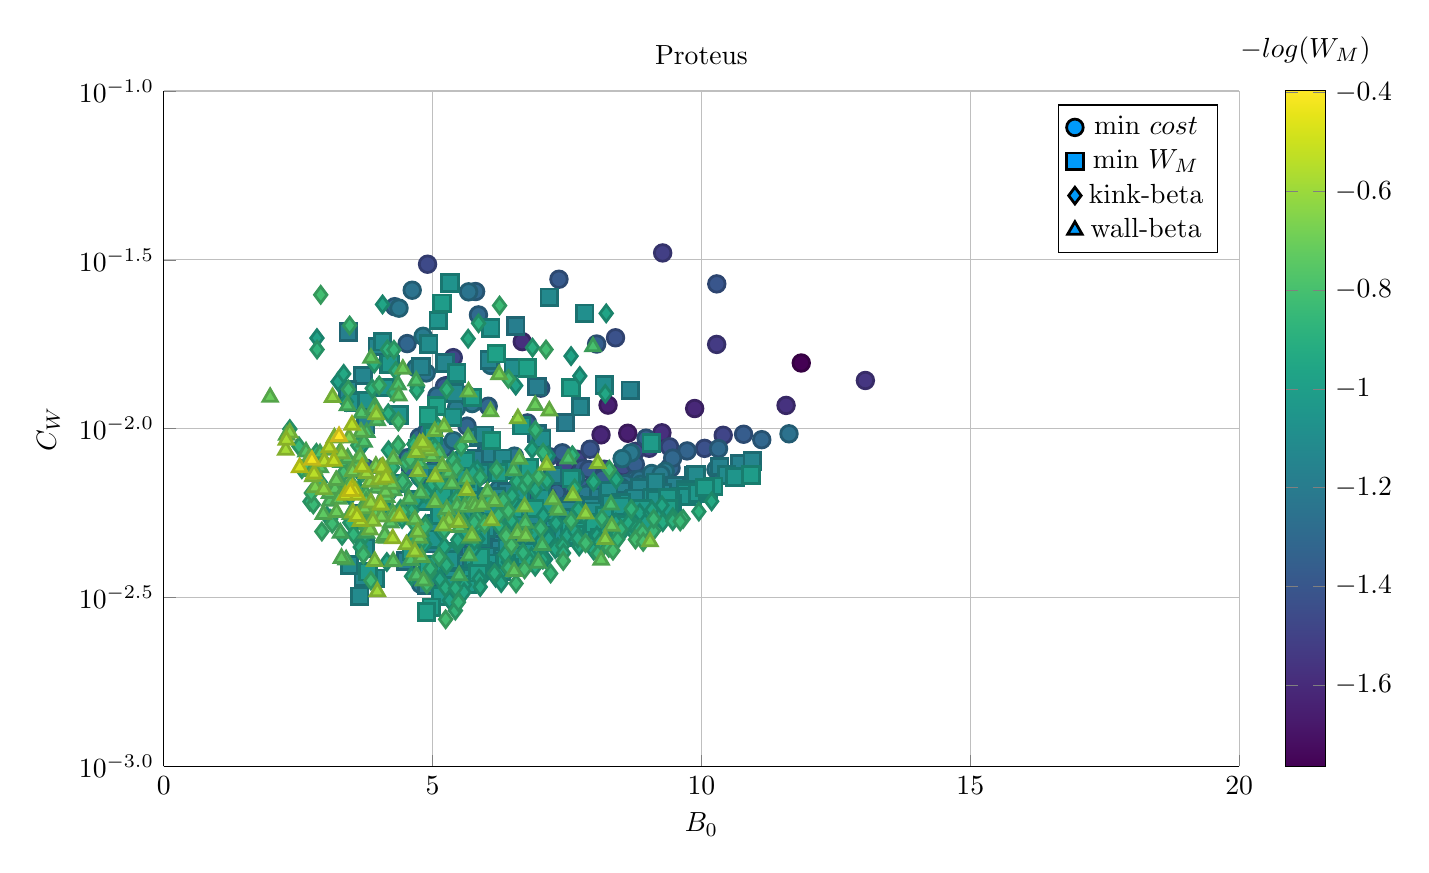
\begin{tikzpicture}[]
\begin{axis}[colorbar = {true}, height = {101.6mm}, ylabel = {${C}_{W}$}, title = {Proteus}, xmin = {0.0}, xmax = {20.0}, ymax = {0.1}, ymode = {log}, xlabel = {${B}_{0}$}, {unbounded coords=jump, scaled x ticks = false, xticklabel style={rotate = 0}, xmajorgrids = true, xtick = {0.0,5.0,10.0,15.0,20.0}, xticklabels = {0,5,10,15,20}, xtick align = inside, axis lines* = left, scaled y ticks = false, yticklabel style={rotate = 0}, log basis y=10, ymajorgrids = true, ytick = {0.001,0.0031622776601683794,0.01,0.03162277660168379,0.1}, yticklabels = {$10^{-3.0}$,$10^{-2.5}$,$10^{-2.0}$,$10^{-1.5}$,$10^{-1.0}$}, ytick align = inside, axis lines* = left,     xshift = 0.0mm,
    yshift = 0.0mm,
    axis background/.style={fill={rgb,1:red,1.00000000;green,1.00000000;blue,1.00000000}}
, colormap={plots}{rgb=(0.26700400,0.00487400,0.32941500), rgb=(0.27794100,0.05632400,0.38119100), rgb=(0.28291000,0.10539300,0.42690200), rgb=(0.28229000,0.14591200,0.46151000), rgb=(0.27619400,0.19007400,0.49300100), rgb=(0.26514500,0.23295600,0.51659900), rgb=(0.25042500,0.27429000,0.53310300), rgb=(0.23360300,0.31382800,0.54391400), rgb=(0.21813000,0.34743200,0.55003800), rgb=(0.20123900,0.38367000,0.55429400), rgb=(0.18555600,0.41857000,0.55675300), rgb=(0.17117600,0.45253000,0.55796500), rgb=(0.15772900,0.48593200,0.55801300), rgb=(0.14618000,0.51541300,0.55682300), rgb=(0.13374300,0.54853500,0.55354100), rgb=(0.12346300,0.58168700,0.54744500), rgb=(0.11948300,0.61481700,0.53769200), rgb=(0.12632600,0.64410700,0.52531100), rgb=(0.15014800,0.67663100,0.50658900), rgb=(0.19109000,0.70836600,0.48228400), rgb=(0.24607000,0.73891000,0.45202400), rgb=(0.31192500,0.76782200,0.41558600), rgb=(0.37777900,0.79178100,0.37793900), rgb=(0.45867400,0.81636300,0.32972700), rgb=(0.54552400,0.83803900,0.27562600), rgb=(0.63690200,0.85654200,0.21662000), rgb=(0.73088900,0.87191600,0.15602900), rgb=(0.81457600,0.88339300,0.11034700), rgb=(0.90631100,0.89485500,0.09812500), rgb=(0.99324800,0.90615700,0.14393600)}, colorbar style={title=$-log( W_M )$}}, ymin = {0.001}, width = {152.4mm}]\addplot+[scatter, scatter src=explicit, only marks = {true}, color = {rgb,1:red,0.00000000;green,0.60560316;blue,0.97868012},
draw opacity=1,
line width=0,
solid,mark = *,
mark size = 3.0,
mark options = {
    color = {rgb,1:red,0.00000000;green,0.00000000;blue,0.00000000}, draw opacity = 1.0,
    fill = {rgb,1:red,0.00000000;green,0.60560316;blue,0.97868012}, fill opacity = 1,
    line width = 1,
    rotate = 0,
    solid
}] coordinates {
(11.855851167264671, 0.015650867313707448) [-1.7651507846396934]
(8.62894306410229, 0.009694646552347688) [-1.652530796858066]
(8.262669569295957, 0.011744038729478485) [-1.647000146345283]
(8.132345586482765, 0.009590177278586947) [-1.6184546481250472]
(9.87352129314419, 0.011474300333025303) [-1.6124908438767973]
(9.26466071494926, 0.00972401084478665) [-1.5828949402967583]
(6.667811597046653, 0.018106858351787505) [-1.577618500437912]
(11.573395463568893, 0.011719738653164523) [-1.56873554690934]
(5.264528343635174, 0.013419897432724169) [-1.5599002750009094]
(13.048135395345042, 0.013892471464509717) [-1.5518482038436605]
(10.282796584070674, 0.017767343192357253) [-1.5302287668791192]
(9.278542294221232, 0.033146306422516245) [-1.5115301730224102]
(7.5044360623009565, 0.007510212646674021) [-1.5013825191439996]
(9.02784009554164, 0.008751202105526691) [-1.4958902811815062]
(8.710683108208965, 0.00816949735167802) [-1.4892617900728689]
(7.687377168804008, 0.008118078139228204) [-1.4884348201277007]
(10.404534949568816, 0.009559158760396884) [-1.4866425610729714]
(5.384524713145202, 0.01623184139531336) [-1.4835478223239928]
(7.472857057569771, 0.007837831837729894) [-1.4780728724015184]
(4.906484287411937, 0.03069401611625924) [-1.4650031348255397]
(7.111580297007043, 0.006765803188842749) [-1.4601242927308113]
(8.773685022223647, 0.008568870415676909) [-1.453691298071198]
(8.545510256202396, 0.007723927816166263) [-1.4489094778079963]
(7.070436548811644, 0.006162431971740805) [-1.432973868001932]
(6.884154096232421, 0.006329451983138475) [-1.4325147285303634]
(9.405921329983288, 0.008839617844718544) [-1.4268866569895065]
(10.057985274469397, 0.008744700190770928) [-1.4268347679685771]
(8.401821549997786, 0.018590297650719324) [-1.4237681445033143]
(8.189937032371649, 0.007587250291191641) [-1.4234658725845162]
(8.234578254729767, 0.007390656211515189) [-1.4109108269606008]
(7.92991212471289, 0.008694085637837138) [-1.4079262096010774]
(6.59839258184741, 0.00634066157530613) [-1.407330123320285]
(10.284931156770094, 0.026840973164111593) [-1.3996791570309395]
(7.3137838143058795, 0.007040053838733538) [-1.3974870797438]
(5.221820332167986, 0.013359280479800206) [-1.3946269662443698]
(7.785957307166937, 0.007634837530984513) [-1.3905305073664083]
(7.069469201177765, 0.006488653571629467) [-1.3895960301339119]
(6.200523563918331, 0.00554611680879456) [-1.381931002288656]
(7.340133149046422, 0.00695131625200887) [-1.3818272949203658]
(7.349866215424601, 0.027704627448181397) [-1.3812563757949996]
(7.351199097200025, 0.00681167564679013) [-1.379699079550137]
(8.120289345307025, 0.006715817539753603) [-1.376650573885692]
(7.90274300232169, 0.00757067906104037) [-1.3758581110553065]
(7.565484576443418, 0.006499559071472007) [-1.375220700855124]
(7.688718501611012, 0.00646934556613389) [-1.3742348635950123]
(7.005633077388933, 0.0063267927368600325) [-1.3713423550361032]
(7.166534585210968, 0.008267480512087599) [-1.370057699317172]
(5.695615872659735, 0.004988896324536347) [-1.3686239973313072]
(6.620180775083285, 0.005540386026064644) [-1.3680076928767484]
(5.712356159098289, 0.005024205798518008) [-1.3672266212882762]
(10.783439028923059, 0.009628839399324697) [-1.3667105305870977]
(6.000471468140266, 0.0050592629231849704) [-1.3651176317240314]
(8.050752136473724, 0.017814080806893125) [-1.3612722200713383]
(8.77043990632116, 0.007840171434328094) [-1.360737823431438]
(7.010340303297389, 0.013182987051350502) [-1.3596008789905631]
(7.295294539644262, 0.006730765435871485) [-1.3568098625263256]
(6.641599582701438, 0.005632641769207446) [-1.3562925407270994]
(6.645748730966029, 0.005613911931897123) [-1.3540300242042478]
(6.054699810485283, 0.005176189759381431) [-1.3527684291391184]
(9.401252816575663, 0.007678792615766904) [-1.3513432280511455]
(5.581708167132495, 0.006888425944911811) [-1.3508742741062625]
(7.803535098905909, 0.006674090356682625) [-1.348444904526092]
(6.76411548346407, 0.010402669872398145) [-1.3482429808137002]
(8.969455503638764, 0.009376571407375644) [-1.3481015746033576]
(5.634510628688515, 0.012583797530216616) [-1.34746159692277]
(8.156032796881272, 0.007115527316776566) [-1.3450418873098828]
(7.056939291922313, 0.006464286011476574) [-1.3449397649071608]
(7.240799475525162, 0.006186516144095541) [-1.344834769873685]
(6.571134452649435, 0.0053864817732829605) [-1.3436955024234147]
(7.4120702527384665, 0.00848434463520388) [-1.3426163725681677]
(5.934011898969639, 0.004938310227983135) [-1.3374912582230194]
(7.37766442956072, 0.006636608478826529) [-1.335539302100867]
(5.026669706190863, 0.007606581585076429) [-1.3352915983538123]
(6.825792187162438, 0.006029019944814239) [-1.331337874103357]
(9.732916904654346, 0.008594819258321628) [-1.3310780697195672]
(5.698038434377145, 0.004728216221281147) [-1.3292068036291638]
(6.854283769326888, 0.005953363383436291) [-1.32828646244698]
(4.7527705925878685, 0.009441137210103956) [-1.3280975618898123]
(6.452485475407575, 0.005079524630506098) [-1.3278697867431468]
(6.6282734062471, 0.005749625528658903) [-1.327757292865828]
(7.362442088263758, 0.006249734903697681) [-1.3253106415861637]
(6.357926345811093, 0.005155209960292018) [-1.3237407060184172]
(9.434691757978365, 0.007650804529712704) [-1.3217246458754282]
(5.945683748997239, 0.004926318213851794) [-1.319376268743699]
(5.716699212704698, 0.004774448071559269) [-1.3182101821558738]
(7.9999703999657505, 0.0066268624262571275) [-1.31770129332637]
(4.526018058829261, 0.017867829271260238) [-1.3171626271127284]
(7.307142270921693, 0.006479743346210051) [-1.3144438328362922]
(5.64022055353738, 0.010177994071422254) [-1.314397397461996]
(11.121291715489328, 0.009279261565995508) [-1.3134452963620502]
(6.890660641840135, 0.005896178522672516) [-1.3126768401499638]
(5.8496112618323926, 0.007223214696135702) [-1.3123916957087167]
(3.755618871416242, 0.007643344629724278) [-1.3117090270675453]
(6.965828665871357, 0.0062843154751196315) [-1.3112976001573549]
(7.132942553696917, 0.006316305209750007) [-1.3102933400586538]
(6.034623082086722, 0.011655743235665423) [-1.3084666426112759]
(9.464190150712176, 0.008181643780093392) [-1.3081739820914746]
(6.735484315816856, 0.005920113041607297) [-1.3081169022767745]
(6.329532230716051, 0.005266304291939928) [-1.3075986397555424]
(6.949512174456946, 0.0056632699287416785) [-1.3038897119548887]
(5.7123865302563095, 0.004515583648974614) [-1.3034916079905217]
(4.588431546307119, 0.00762405310841983) [-1.301506470226052]
(5.8529754306366, 0.021723513711501174) [-1.2978787946122285]
(6.763583440942078, 0.005860560202229156) [-1.297460949292816]
(5.79974352272628, 0.02547444831481485) [-1.2953226778576867]
(4.294506467374343, 0.022974551007964673) [-1.2951062787178942]
(10.317711969577175, 0.008727794605170999) [-1.2946978796261759]
(7.030442720189729, 0.00606442154900928) [-1.293243062455323]
(6.3155245633398005, 0.00478216163852665) [-1.2916316854649297]
(5.594153930448576, 0.004505685536187866) [-1.291573412415986]
(7.0608047385200905, 0.006201757851874389) [-1.2910367642815292]
(8.746159160738731, 0.007056272547770033) [-1.2894268757747884]
(5.790961836119614, 0.004812007322004063) [-1.2891780169645117]
(7.13931972393237, 0.005900795309436559) [-1.2883016772579983]
(5.642350264315365, 0.004575860387174974) [-1.2877120777365891]
(5.500511487756749, 0.007501625869556503) [-1.2825608117529994]
(5.1870060839860015, 0.004048206616482656) [-1.2803416949249293]
(5.0793762257146975, 0.012501014524680899) [-1.2790944723531177]
(4.900710067477188, 0.009849033693022476) [-1.2789599032268324]
(5.416336002756713, 0.004266328381972482) [-1.278637308935949]
(7.047880217226236, 0.00602317781329061) [-1.2752962713941192]
(4.537987048593646, 0.008202673797589401) [-1.2724318730764337]
(6.7947527911354095, 0.005313590913225172) [-1.26778944603233]
(7.547856502776895, 0.005746237915345085) [-1.2652894696394015]
(8.337373800803634, 0.0063394092295352205) [-1.263844406219344]
(5.839234828237175, 0.004670640784960837) [-1.2622412045786418]
(6.307588148065544, 0.005025369604276285) [-1.2622057750392766]
(6.369182324037021, 0.004715175023029078) [-1.2568407944078956]
(7.25221896281004, 0.005515822538041083) [-1.2564369672634057]
(5.207422458409709, 0.008763742702873716) [-1.255580803936347]
(8.846964102011665, 0.007090160917314494) [-1.2542825781236586]
(11.62801313878366, 0.009658252430988482) [-1.253606675738751]
(6.586437041421525, 0.005078101074449218) [-1.2533258835374417]
(5.896819232149536, 0.004668333949768413) [-1.252740293490489]
(7.218625057420257, 0.005623439530060779) [-1.2512906609771755]
(4.770007649977626, 0.007192663750971734) [-1.2505906665339703]
(6.391248250395476, 0.004753912504004936) [-1.2505667349102745]
(6.722228809625436, 0.00547669175115548) [-1.2505409706978425]
(5.9975644347104575, 0.008585550973626429) [-1.2504311283223648]
(6.220483255591395, 0.00536142422310656) [-1.2495193060816674]
(7.131398255569569, 0.005891517799670805) [-1.2472203996667584]
(4.620896334693883, 0.025703839631456088) [-1.246340221801285]
(5.634708074324937, 0.004426672964739238) [-1.246337044553182]
(6.0053836269885, 0.004733745531528537) [-1.2444533586241864]
(6.122472771064873, 0.004373459187272198) [-1.2410504069560844]
(4.881468969197191, 0.014622918962551527) [-1.2404616678069278]
(5.669873863181108, 0.025422666134658947) [-1.2402101811954278]
(9.159921449108527, 0.00699405114862055) [-1.2399625556579728]
(6.619988989498716, 0.005459593535350185) [-1.2395775558220574]
(4.0721743569002395, 0.006780135026174841) [-1.238968027160994]
(8.487125648729805, 0.006381273355008305) [-1.2381935518916032]
(5.785136288326493, 0.005454977773134567) [-1.2372164242860222]
(7.805870043590986, 0.006162937475975255) [-1.2359322527835273]
(6.521775930847536, 0.008295248979234676) [-1.2345953253761524]
(7.299795216034374, 0.005661235915534237) [-1.2333782101635051]
(6.654376116038794, 0.005116145429327062) [-1.2329256482335589]
(8.586321868785943, 0.0068738253515159406) [-1.2318041138227]
(5.871716076416853, 0.007759607253139788) [-1.2286780396839752]
(5.525881431830733, 0.004270512991179436) [-1.225800447150557]
(4.37566370657649, 0.022744869820021597) [-1.2237626122718148]
(5.386416012885563, 0.009221148903357415) [-1.2192315569877235]
(5.735606858683557, 0.011868028475244749) [-1.2191811590789894]
(8.68706974133124, 0.008481483201532794) [-1.2185680785343938]
(8.63032181590475, 0.00622802822970762) [-1.2179132583990178]
(8.508158073563377, 0.006703260233628488) [-1.2171472173843672]
(7.953691408978824, 0.00633213628058925) [-1.2167448502658762]
(6.081331959057098, 0.015392818825938645) [-1.2162995250149307]
(5.225401290559421, 0.003872910530196867) [-1.215703789534109]
(5.988978974443945, 0.004720977485089404) [-1.2156312790675603]
(9.073087462786646, 0.00736963569440644) [-1.2145283350978044]
(7.217725198328268, 0.005383150867826381) [-1.214317974252912]
(5.536577745729214, 0.004178935326843822) [-1.2138536176262873]
(4.776559777248383, 0.0034641548226198885) [-1.2119360055173332]
(5.211688187540344, 0.0038140534914709043) [-1.2104347246988538]
(10.269380266980404, 0.007570292211977012) [-1.2084631186053005]
(6.918845939903695, 0.0052385995930077645) [-1.2083264519217767]
(7.0692693982238906, 0.005083028024589718) [-1.2073346872626274]
(5.874112036399968, 0.004039129704078142) [-1.2071975929322125]
(4.690082401892927, 0.01513911751066285) [-1.2067840670536927]
(7.861161945792819, 0.006395373245847939) [-1.206736577191552]
(9.326423266814658, 0.007483645463069493) [-1.2065799786199445]
(8.029413669351802, 0.005698374888186277) [-1.203843641047789]
(6.959732144718079, 0.005550896360654382) [-1.203724365314369]
(6.960477287319412, 0.005010777712400389) [-1.2024406864855146]
(7.654476699386534, 0.007157947201399507) [-1.2021169810907544]
(4.823547237227045, 0.01877759730610099) [-1.2015933815507112]
(6.062862639710857, 0.004489267037355289) [-1.2014423796656961]
(8.999102001729389, 0.006374667856956503) [-1.2011965112492808]
(7.2717504340335415, 0.00572395742880883) [-1.2005427289121806]
(6.227413325881237, 0.0066192080125215165) [-1.1994215784439877]
(9.247503176233229, 0.007316062816603203) [-1.1975084180232178]
(5.443249511926066, 0.011502671870448664) [-1.1972619972446426]
(6.742357647461489, 0.005266662336518346) [-1.1967371969067386]
(5.926964832086266, 0.004368135902166705) [-1.1965134818457024]
(8.524769827029726, 0.008154332104698897) [-1.196084536648355]
(8.867575034400405, 0.006843978332329513) [-1.1943424204563022]
(6.457339766119646, 0.005029914775543452) [-1.1908054127888088]
};
\addlegendentry{min $cost$}
\addlegendentry{min $W_M$}
\addlegendentry{kink-beta}
\addlegendentry{wall-beta}
\addplot+[scatter, scatter src=explicit, only marks = {true}, color = {rgb,1:red,0.00000000;green,0.60560316;blue,0.97868012},
draw opacity=1,
line width=0,
solid,mark = square*,
mark size = 3.0,
mark options = {
    color = {rgb,1:red,0.00000000;green,0.00000000;blue,0.00000000}, draw opacity = 1.0,
    fill = {rgb,1:red,0.00000000;green,0.60560316;blue,0.97868012}, fill opacity = 1,
    line width = 1,
    rotate = 0,
    solid
}] coordinates {
(7.4724590738720655, 0.010422279639263054) [-1.1890033537880158]
(6.938996985119089, 0.009658294464102987) [-1.1883675827161198]
(6.9393893920794385, 0.013313745665171912) [-1.1879538738656286]
(6.377850385556073, 0.006487414571263668) [-1.1878029685724296]
(6.547487324963764, 0.020145877705477357) [-1.186260879134981]
(8.029613686159495, 0.005801884747670386) [-1.1859242026174677]
(5.6874025972941205, 0.004217349677698315) [-1.183889066210908]
(7.827309596895398, 0.0058827996938258294) [-1.1830291222504283]
(5.8219713598117036, 0.008160599297710009) [-1.1826268505607591]
(6.946718058585209, 0.004857174007518612) [-1.182365307189366]
(3.434094114791118, 0.01935279381255584) [-1.1822251925764147]
(6.23809783755075, 0.00447855648592392) [-1.1813612663460882]
(5.88781791976068, 0.00428725320402622) [-1.1785285195809967]
(4.505121226933233, 0.004053651772674214) [-1.1775655951090325]
(6.553162158329651, 0.005121496915389368) [-1.17705398157876]
(5.8303432949169745, 0.005890819973806921) [-1.1767452937515073]
(8.807822926389145, 0.006104718148251412) [-1.1766083315756861]
(4.18691738643155, 0.01556268699280997) [-1.173888237216638]
(7.55203601905607, 0.005882961839613334) [-1.1734465174435744]
(5.819836385827624, 0.005961179911412564) [-1.1729466514857931]
(9.116693027577789, 0.006287276174883399) [-1.172839252676928]
(3.659189590525744, 0.005599267038542826) [-1.1727769211527406]
(7.004035835152084, 0.005070632392189801) [-1.1727372361954858]
(4.897086463141796, 0.003434292526080427) [-1.1726542785062386]
(8.087708955601924, 0.0062657093568900535) [-1.1703764252048678]
(6.7024429891400565, 0.004942047034638912) [-1.1699166462753263]
(5.893015258208656, 0.004183590560340062) [-1.1681831393061217]
(7.479710666339309, 0.005170881199231806) [-1.1671080842733117]
(9.508375514310952, 0.006777996547666784) [-1.1655606692177785]
(6.075560203652315, 0.008402469668507205) [-1.165303541813206]
(6.61932998550545, 0.004666935296152095) [-1.1643973078802388]
(6.286558265163782, 0.004663766235492665) [-1.1632535008384055]
(5.050068824721165, 0.004566940606242733) [-1.1631989573193973]
(7.688714523679582, 0.0054331000812183365) [-1.1630392685982025]
(8.505800422917172, 0.006544368204474158) [-1.1625753891662707]
(8.975209897762664, 0.006511116933487475) [-1.1617936783337066]
(8.380983437312786, 0.006126048639979384) [-1.159367616011031]
(8.67470730810651, 0.012995381528200805) [-1.1593260324319568]
(5.960621269295445, 0.004013416769217783) [-1.1592024857112633]
(6.282535161243701, 0.004530529794416821) [-1.1590403977294572]
(10.712436821713085, 0.007867971330715704) [-1.1589428109110296]
(7.099415207654768, 0.005330271588661515) [-1.158451320077056]
(10.3395352744249, 0.007724720119696045) [-1.157468772898154]
(6.536306152444655, 0.004436262085616985) [-1.1570637161067505]
(9.855000808062698, 0.007249642226094706) [-1.1563966451418943]
(5.856384724795581, 0.009420901412013665) [-1.1561531921827275]
(7.454679880823048, 0.0057898611640113395) [-1.1538328200442942]
(5.14753239685863, 0.007237376261288284) [-1.1525173430901554]
(6.856563325018079, 0.004881019954742076) [-1.1522162283529644]
(7.618840457764884, 0.0059379940430840635) [-1.151968932860403]
(8.398440991699191, 0.0061407721476487214) [-1.1511586507355254]
(4.781165601129724, 0.015255960449664327) [-1.1509834966159156]
(6.247011281135245, 0.004419080970160178) [-1.1503660387736743]
(3.7553680100049234, 0.01032617135589161) [-1.1500086948877408]
(5.5152996897670015, 0.004014883666259908) [-1.1494080253790357]
(7.800728278542519, 0.005291422749753008) [-1.1493093072503229]
(6.054088477025007, 0.01598351560152435) [-1.1489823622220707]
(5.411295562966824, 0.003915099463846501) [-1.1484511044037433]
(7.052045109627868, 0.005020529922825154) [-1.1483999797493492]
(5.28488049549897, 0.0034947010100993764) [-1.147064765638366]
(7.62011089503286, 0.005859550653426385) [-1.1465028274549764]
(7.468210164743146, 0.005641165149475234) [-1.144883586902141]
(5.595946792423691, 0.007176119328254024) [-1.144368544047569]
(10.943656185786155, 0.00802165691682325) [-1.1435280806157744]
(7.908061023064291, 0.005447269817044685) [-1.1433393449411435]
(8.854582349908517, 0.006668732693209443) [-1.143332108158641]
(6.549837080949351, 0.004886014774808058) [-1.143184585873657]
(3.9729755898485215, 0.017515494611674454) [-1.1428249654095861]
(3.703954177548893, 0.014377117697389604) [-1.1427984862828113]
(3.4213090828497417, 0.013005276311642224) [-1.142397010267489]
(6.02709699747974, 0.005929095379259443) [-1.1423708774410877]
(5.231750077921478, 0.01565086593371781) [-1.1422424769576425]
(7.2349136535832095, 0.007266091038483963) [-1.140012696356206]
(7.647205004097057, 0.005840600330748377) [-1.1399465227440013]
(6.532016233135844, 0.00480284773560221) [-1.1387943392990294]
(7.523885505796154, 0.005752426766742318) [-1.1382802201938975]
(7.750130276532692, 0.011612930840038163) [-1.1380314198362265]
(9.276469763067444, 0.006446360072583165) [-1.137892443914052]
(5.952941013085345, 0.009562541252399106) [-1.1311113631375915]
(7.951426521304668, 0.005743536904522906) [-1.1302954325651586]
(5.952653119927932, 0.0041760314888273755) [-1.1295543261638465]
(8.253192497448524, 0.006161648966500728) [-1.129462828049983]
(5.512192429439468, 0.00369116854025651) [-1.1277963061708562]
(6.180741676638315, 0.006278926396423389) [-1.126807171194116]
(6.608627477861355, 0.004487529275565533) [-1.1267021554022474]
(9.14457555501132, 0.006938744439971839) [-1.1265761162904897]
(5.310301950330671, 0.004304336836767321) [-1.1261385034152473]
(7.969320198807478, 0.005917258047258142) [-1.1260458936236624]
(7.954215183655014, 0.005885263457738176) [-1.1250537668582923]
(6.771595293849517, 0.005616858230043609) [-1.124511019242948]
(6.641944516873176, 0.004843731890681865) [-1.1236988869720232]
(6.896134858333351, 0.005173923137495115) [-1.1235064786985465]
(3.7132325707792995, 0.003624821435760545) [-1.1232730371267585]
(4.936839162331792, 0.007429853985811719) [-1.1231293548483412]
(6.555316024199809, 0.005231942783984398) [-1.1209978185544383]
(6.304604592673814, 0.008169617815892689) [-1.1196911148335087]
(8.737416781995437, 0.0061580609115664325) [-1.1194748634113345]
(6.123815672401932, 0.004188882178419093) [-1.119418152841014]
(8.324353852438948, 0.005791769416647159) [-1.1191123923650526]
(6.830685941792606, 0.004931972266091366) [-1.1181736482095217]
(8.279157421008941, 0.005611347227289511) [-1.1176702646643628]
(7.172394160745635, 0.024480989089009208) [-1.1175403888423328]
(6.753756430979739, 0.004518885765871233) [-1.1174827013795072]
(8.76524294869496, 0.0062233325455323925) [-1.1174414411464733]
(5.952289891041446, 0.006299808378708293) [-1.1171134960728113]
(6.523754565443294, 0.004568184715721437) [-1.1171111976535804]
(5.4096290381473375, 0.012757776435747556) [-1.1168806186241906]
(9.896916686410892, 0.007305420869085463) [-1.1160945644374545]
(8.286804128590813, 0.005340773800773009) [-1.1139896885893594]
(5.399012890266871, 0.0036233885329560954) [-1.1123768792739945]
(8.296167355721272, 0.005311493039288053) [-1.1112153482766423]
(6.778775360762903, 0.0045000578497955725) [-1.1111283014916062]
(3.642453456441478, 0.003188662256079057) [-1.1108869662710774]
(6.918579935305505, 0.004842654136629077) [-1.1089922492653659]
(6.5071710234613676, 0.00452032863173795) [-1.108391782497311]
(7.258592477367294, 0.00535669926333167) [-1.1082929384878708]
(6.6776055936353265, 0.004745534590751309) [-1.1074346113685616]
(5.3226296796509205, 0.004323464728471098) [-1.1074227437950106]
(10.46985584146923, 0.007293078759243216) [-1.1069130893453907]
(3.4547855533452156, 0.003945456212149148) [-1.106325178133445]
(7.57975455174028, 0.004982808461571556) [-1.1060035644106432]
(5.06842585608741, 0.0052409052861536465) [-1.1038776732161713]
(5.698043204630489, 0.0065314531396132094) [-1.10351060592976]
(7.734654274692709, 0.005173060010686301) [-1.1022315889718237]
(6.228402773452205, 0.005951424789746293) [-1.1016702257969113]
(5.288893434740895, 0.007437806150470808) [-1.100448826904311]
(7.254453932047169, 0.005288339533793414) [-1.0998565094908217]
(6.807046489565401, 0.004337170224988449) [-1.0995498480529582]
(8.496667761878552, 0.005750254423520601) [-1.0992970719713648]
(6.506723144546308, 0.004423364554484401) [-1.0987351440216522]
(8.273277101596172, 0.006535275113176343) [-1.0983869460625248]
(7.024499917691516, 0.006822630998366228) [-1.0977261444257258]
(4.929559505548113, 0.017828562633364364) [-1.0969882385788774]
(6.546519891753608, 0.004407786879742766) [-1.096807077081938]
(6.299458688060015, 0.0041501216036249275) [-1.0962033310727437]
(5.917588131126826, 0.003972749736578854) [-1.0948458082881816]
(6.5027787367036485, 0.015155543307471772) [-1.093965318294314]
(8.191093731826841, 0.013471957430229371) [-1.093275686079877]
(5.765417917352738, 0.003923510470624812) [-1.0931318196649105]
(4.067683728143941, 0.01811006730780237) [-1.0926393639694263]
(5.643295069658257, 0.005671433069083637) [-1.09199330517098]
(5.33448260992027, 0.0035546432563184145) [-1.0916603258728452]
(5.996010919360583, 0.005082501155756355) [-1.091508438458307]
(6.130249778803564, 0.003922207642532424) [-1.0911853630489914]
(5.152309500808404, 0.007129588907950501) [-1.0896526200520398]
(6.613976143688219, 0.004468466025444819) [-1.088663441639713]
(7.828710312153846, 0.021949864805969728) [-1.0877780715734315]
(7.029871400370792, 0.009322832924906896) [-1.0870739196827126]
(6.6598420793586, 0.004672088916974179) [-1.0855818982110972]
(6.33097870945106, 0.004039319528471343) [-1.0844715994400023]
(7.702268833143657, 0.0053439960085053) [-1.0842780595786392]
(6.084754710909704, 0.005760793758021615) [-1.084266572782003]
(7.98999393987453, 0.00569380985136289) [-1.0839928767281124]
(5.068992476376386, 0.0039349920083461085) [-1.0828594792618813]
(9.086048642306793, 0.0062405207423892875) [-1.082853352734588]
(7.44906676523106, 0.0054577800846403015) [-1.0824719035597]
(5.375575122544495, 0.0035809652689903063) [-1.0824709528228211]
(7.386984140765724, 0.005148297391297789) [-1.0814366033908964]
(9.702271536107535, 0.006582162000449632) [-1.0809878234039578]
(9.614854186704672, 0.006301853688415234) [-1.0808972954130593]
(4.645688111866446, 0.006161790226168522) [-1.0797863646031054]
(3.927334262139488, 0.0036086053477567665) [-1.079163153355685]
(6.963971610592974, 0.004793357206410555) [-1.0780309855478056]
(8.244956752748422, 0.0054298508521766365) [-1.076806285491668]
(5.769697532800943, 0.00604411217248383) [-1.0765985094568509]
(7.283344319549832, 0.004828662165485411) [-1.0760641298404754]
(5.392578394594405, 0.005661819547798889) [-1.0757730303287785]
(3.7434225317786316, 0.00443044659495794) [-1.0744056068515366]
(7.7252366425534715, 0.005467468655559742) [-1.073726482715373]
(8.506016241294386, 0.006046667097602973) [-1.072815333291583]
(5.722077224788854, 0.006315687038558954) [-1.0718638391063322]
(3.5290681872248832, 0.011989877345034696) [-1.0710072465261937]
(5.408389828424612, 0.006287200186056995) [-1.0706716976099708]
(5.880603880610476, 0.00739594343637032) [-1.069478881808043]
(3.770984054785403, 0.012080600310741674) [-1.0679830462657767]
(9.144669371614333, 0.006138341400017388) [-1.0670572282884458]
(5.3325423351198395, 0.004085658341340117) [-1.0667391835901658]
(8.316799187366927, 0.006004004929014098) [-1.066302608545655]
(6.389619437625667, 0.004440975162005993) [-1.064104157833971]
(5.324355765249537, 0.026972932068461592) [-1.0640878812065675]
(6.511622532652898, 0.004395996587917252) [-1.0635820925869255]
(6.911249511094287, 0.004423420241739423) [-1.062988318250961]
(7.502962627592097, 0.00480727122317776) [-1.0628036997189863]
(5.469724443246719, 0.0034131330547271113) [-1.062700357913494]
(5.706475165604361, 0.0036974585830479817) [-1.0626514373993834]
(7.276669037534987, 0.004776499853086686) [-1.0610739421064752]
(6.526975357350624, 0.004144297606935685) [-1.0588352037418618]
(5.105089902831069, 0.0209014980088616) [-1.0585986545827941]
(4.374531653432859, 0.010988948677442597) [-1.057135771526312]
(4.122473679442906, 0.013241941603829825) [-1.056315661795303]
(6.078673477412938, 0.019862106250452566) [-1.0562734967702754]
(7.427558910001991, 0.004858658731965693) [-1.0561257856094448]
(7.01015270925273, 0.006223828461257365) [-1.0559814704124602]
(5.014809023336614, 0.004706089102701761) [-1.0555859489072712]
(6.029077134394886, 0.003994614402213268) [-1.0549803415205259]
(9.718000396033032, 0.006463993798881436) [-1.0545713902023608]
(5.896086527792721, 0.0038990516235787613) [-1.054205756099488]
(10.62632239203378, 0.007195479612398366) [-1.0536290024409787]
(9.830251746280974, 0.006286763322784177) [-1.0533216125601341]
(5.653429182632709, 0.004822724612666477) [-1.0529307720930816]
(7.148582094551358, 0.005656264568736301) [-1.0525850668019536]
(9.721783343528084, 0.006295530789348686) [-1.052552508886994]
(6.4747129291886205, 0.007550888758433211) [-1.0509835312174363]
(7.5553171987129115, 0.004904482654727138) [-1.0508250621973283]
(5.689433662550519, 0.006571304536184572) [-1.050680345054969]
(6.819358408267933, 0.004560195418506711) [-1.0506245233592775]
(5.372500908480495, 0.01080264515897382) [-1.0505217359121972]
(9.464104357867244, 0.00597835329976134) [-1.049317623712287]
(9.421645636318559, 0.00605275476812188) [-1.0490747591885061]
(6.83923495211403, 0.004511808104116367) [-1.0489907539423449]
(7.595014509377157, 0.0049153150140211965) [-1.0478434867034416]
(6.9492853284169565, 0.004616652674773231) [-1.0473758850488442]
(6.631954997333512, 0.006447737760929581) [-1.046767629611379]
(4.836574702453568, 0.006114416229637186) [-1.0460742739305466]
(5.447392742867525, 0.01461141466329314) [-1.0428746875530057]
(5.278008805745069, 0.0034297894059699906) [-1.0409932776852704]
(6.869290933859089, 0.004324846597058025) [-1.040720375777512]
(4.388359570069462, 0.0068957525832947) [-1.0400494553390642]
(7.730136216039545, 0.0047742837106654985) [-1.03963800286999]
(5.097390647393597, 0.0070972253563865) [-1.0394862991533038]
(5.705197239891871, 0.006107051538135721) [-1.0391370640013136]
(4.211114439903267, 0.015503036624972183) [-1.038354289214968]
(9.925180494788561, 0.006445735380428859) [-1.0380750082543837]
(8.392824243874195, 0.005205902574339689) [-1.0370263081612092]
(7.973811270774484, 0.005283195240312258) [-1.0365321066837632]
(8.49921904371083, 0.005892181423629392) [-1.0364145571368009]
(6.655649338522086, 0.010214094301379546) [-1.0358730287795153]
(6.272206414918943, 0.003781581128188247) [-1.0352797650690977]
(9.40142074331525, 0.0061316127141858145) [-1.0352425491421158]
(4.6061758509773245, 0.004345014451914255) [-1.0335536367675167]
(5.764426452876033, 0.00415632052734694) [-1.0319535365225938]
(9.372888478292797, 0.006253917955260214) [-1.031638330454266]
(5.729013310777877, 0.003613822408322808) [-1.0316283345953763]
(5.883030813164119, 0.00478160347928963) [-1.0312630056422283]
(6.556479558238363, 0.004326998549376461) [-1.030801418278412]
(6.395724956994062, 0.006039359373565179) [-1.0301227610636083]
(5.139256557257989, 0.005550817437725965) [-1.029015666765989]
(10.123332193763748, 0.006583295742064639) [-1.0288573869793878]
(6.568561456688728, 0.004204292638824563) [-1.0245024368116802]
(5.6039086370880105, 0.007145400138218064) [-1.0231385619546913]
(7.648719554707365, 0.004789677204757558) [-1.021449027000752]
(10.226601060349507, 0.00675373673736514) [-1.0213127693885564]
(5.153470412653239, 0.003193542226257652) [-1.0209276741398987]
(7.579001576207003, 0.007121099635585821) [-1.0202684704954939]
(3.8015765702844804, 0.0037708668397859442) [-1.0187837906200732]
(8.894908266877893, 0.005805595496214904) [-1.0179738483919518]
(9.066566182501706, 0.009070154520460257) [-1.0169425110693646]
(8.213444606213486, 0.00501503870041615) [-1.0162045101447212]
(10.062564168396998, 0.00670010251636303) [-1.0149810946438107]
(4.727731778507776, 0.008752580219573484) [-1.014353466976016]
(5.174769297851055, 0.023528952793841592) [-1.0140528730661398]
(8.195915051921629, 0.005527004085356763) [-1.0133093427968076]
(7.054369905297556, 0.004778958682375364) [-1.0128360857902137]
(5.031848935370691, 0.003842216867194081) [-1.0126834015105255]
(10.922140692684003, 0.007300503854095673) [-1.0124869131348806]
(5.915584448350069, 0.0038089628255598917) [-1.0084966915198963]
(5.602678326023923, 0.008048423371546378) [-1.005776006726422]
(7.544600594243294, 0.005136336479510988) [-1.0027757315503723]
(4.977942341177753, 0.0029594317443149176) [-1.002422823826331]
(5.642218938318191, 0.003459304695059543) [-1.0023352556688647]
(8.295019648678474, 0.004988217345842403) [-0.9994656987080655]
(7.070940189155582, 0.004649343635980374) [-0.9991953302395459]
(6.226711465325763, 0.007411548557741582) [-0.9991876183275935]
(6.419292049664728, 0.0038831217844692545) [-0.9971256954762724]
(4.887255844769486, 0.0028654321699102935) [-0.9968293366364798]
(7.7523402111694955, 0.004992975570566671) [-0.9965130838642419]
(5.890289877584987, 0.003830578946172306) [-0.9960911988132904]
(7.574296219984337, 0.013215773066776348) [-0.9953080727443692]
(9.012153601445592, 0.005338097758519931) [-0.994764309342816]
(9.386356586964215, 0.005798704578553127) [-0.9941918143808477]
(6.789856926677994, 0.007661762309327555) [-0.9939974184414383]
(5.741492166499531, 0.012372283627325148) [-0.9936895922796631]
(8.093840230774958, 0.0047417231470052315) [-0.9920762514365737]
(8.423301149042322, 0.005175409039233765) [-0.9891335090238219]
(6.5096125388500665, 0.005799134035216279) [-0.988320863141931]
(6.362065295698958, 0.003975692742134705) [-0.9873980470532571]
(6.898795759334327, 0.005803966541873779) [-0.9872638091155089]
(5.86662772167221, 0.005281651647264406) [-0.9871243344745786]
(5.00980677003057, 0.00954881671016918) [-0.9862026242600886]
(6.0980328290063905, 0.009231911938640338) [-0.9851939256634008]
(8.004532839270633, 0.005233428706224578) [-0.9845137991026185]
(6.760939557779194, 0.015110407509335635) [-0.9844063088607684]
(5.192252043701997, 0.006274740712107015) [-0.9843851675543582]
(6.182612803400956, 0.01666579340898781) [-0.9832677624207663]
(8.112468976523042, 0.004743145828135927) [-0.9823156156623659]
(5.841361480008224, 0.003744148435661381) [-0.9817957805945331]
(7.647006952351862, 0.0048552692105239565) [-0.9817262777133879]
(5.077285700891451, 0.01167873981501713) [-0.980944500204026]
(5.883453787587344, 0.004161496814710868) [-0.9808435285359967]
(4.920420200443467, 0.010903168023481107) [-0.9803069086017846]
(8.471906861597214, 0.005187973951951495) [-0.979926239566149]
(4.915731269106913, 0.0039527765780552285) [-0.9799255860420428]
};
\addlegendentry{min $cost$}
\addlegendentry{min $W_M$}
\addlegendentry{kink-beta}
\addlegendentry{wall-beta}
\addplot+[scatter, scatter src=explicit, only marks = {true}, color = {rgb,1:red,0.00000000;green,0.60560316;blue,0.97868012},
draw opacity=1,
line width=0,
solid,mark = diamond*,
mark size = 3.0,
mark options = {
    color = {rgb,1:red,0.00000000;green,0.00000000;blue,0.00000000}, draw opacity = 1.0,
    fill = {rgb,1:red,0.00000000;green,0.60560316;blue,0.97868012}, fill opacity = 1,
    line width = 1,
    rotate = 0,
    solid
}] coordinates {
(5.163569333804058, 0.0049343734079309275) [-0.9797193514246809]
(7.7377435890937285, 0.014326928101993836) [-0.9793649258547107]
(5.770648171127724, 0.004418560150536774) [-0.9793554194238832]
(4.7261265073999565, 0.007133046942930264) [-0.9793399260652301]
(4.749925847834237, 0.004527202123528333) [-0.9786718824413932]
(3.240965863210715, 0.013777079521683793) [-0.9784247640598123]
(8.408728218761828, 0.005278344797288595) [-0.9784156054323705]
(5.20936895107677, 0.004002965553163199) [-0.9772101816150688]
(6.546367069245276, 0.013418113026562503) [-0.9771245449599791]
(6.406431686907994, 0.004027289040267911) [-0.9768013676267739]
(2.8493674862886933, 0.018551171796247393) [-0.9763993914483391]
(4.701597365840406, 0.006130885121857039) [-0.9762949474128021]
(9.199948291326558, 0.005562603331167774) [-0.9759999361809304]
(7.151824598817379, 0.008328856003390762) [-0.9748577786630778]
(7.102409218167167, 0.004109700372311695) [-0.9738966318394574]
(8.195112351068081, 0.004913914166672265) [-0.9734793512186626]
(8.019705338927611, 0.004665122126804512) [-0.9731032751395803]
(4.288110261014516, 0.006640697404806304) [-0.9726016535105552]
(7.158134609952364, 0.004736078134325021) [-0.9724572780741577]
(8.692965677697089, 0.005647304198937851) [-0.9722087723669882]
(7.04081204863579, 0.004389286248628818) [-0.9718244022964762]
(6.172874474865109, 0.0036192646662402627) [-0.970582002945255]
(5.829412829585688, 0.007574170243236733) [-0.9693863160362324]
(7.575254278646649, 0.016406094197261946) [-0.968978562403945]
(6.893566062723393, 0.004910644527520683) [-0.9682987091511867]
(5.843014132287411, 0.004713875842941002) [-0.9661896439247507]
(4.121615844519561, 0.005899389733384474) [-0.96458538139874]
(8.852159273433807, 0.0056286885015633895) [-0.9644132418595727]
(7.329772367480614, 0.004458328702018249) [-0.9642494738631832]
(5.31195688229714, 0.005896947846453336) [-0.9638749980488863]
(3.697832735744159, 0.008919099387898428) [-0.9633607889353855]
(6.250834556973929, 0.003704995647544644) [-0.9628913890413714]
(6.500149334307347, 0.00612171997200749) [-0.9627420883815555]
(5.897610687949902, 0.003560196433315863) [-0.9623524414535783]
(8.228428756399241, 0.02195538724653361) [-0.9620751879990892]
(5.31447757801713, 0.0031037314795763953) [-0.9616273380898692]
(4.624496397148145, 0.004737846584498155) [-0.9614728013262]
(9.047502524734744, 0.0056288454988440186) [-0.9611621976310423]
(3.471426876486878, 0.006420794710655912) [-0.9607076853432408]
(8.055993344424852, 0.004827398822111102) [-0.9600064809118957]
(4.06945875470874, 0.02333271298987377) [-0.9582788764682687]
(7.8112502642797335, 0.005548252171458194) [-0.9582126253448857]
(4.396839446778801, 0.005664193052715976) [-0.9580357625022031]
(7.059156686353003, 0.005536719771654066) [-0.957784719926681]
(6.4485520230870526, 0.003853864382102105) [-0.9569481934101607]
(9.079267570556611, 0.005755412847229535) [-0.9553125817248839]
(6.850175265995453, 0.008689466677368552) [-0.9542931196842905]
(9.265046294027139, 0.0059335279307082415) [-0.9535689234008579]
(5.556145133044266, 0.00540418577910244) [-0.9533577705177119]
(5.606085450842784, 0.004951751523060612) [-0.9524896594035642]
(5.864773049982009, 0.0035965091424978767) [-0.9519498604980341]
(4.871789867074014, 0.005225320910765454) [-0.9518141933322811]
(4.821265154656363, 0.0064487141747247515) [-0.9516817791582881]
(7.49714796909489, 0.004824944888873151) [-0.9503280372896984]
(7.652085089646745, 0.00494548994415281) [-0.9501901690400224]
(3.6090788861115164, 0.005348280279251544) [-0.9501200807106565]
(5.592765892679784, 0.003451161099821506) [-0.9494094470373718]
(8.211654548745017, 0.012679296138241048) [-0.9485432404545778]
(3.4687639943104416, 0.006306624155522614) [-0.9476409244484506]
(4.715290208355647, 0.013277570668597095) [-0.945668217439486]
(3.3968467639253097, 0.012011087422302516) [-0.9455646191283261]
(6.929080513992421, 0.0042225651663969944) [-0.9452539976263535]
(5.753334163582096, 0.007400046119087899) [-0.9445379968061569]
(6.431026814779499, 0.0038853521635503845) [-0.9442842771351952]
(5.13470470595001, 0.003581425300578328) [-0.9439633256599537]
(3.346771982647369, 0.014533706969027229) [-0.9435190061725043]
(7.296199575307953, 0.005251128867230356) [-0.9431579759120018]
(5.584711216656185, 0.0032803092315458883) [-0.9428483368499935]
(5.759317722724291, 0.005138967929828396) [-0.9422331530579936]
(6.2763056958379275, 0.0034905159514662587) [-0.9396609276523904]
(4.148908790420203, 0.004029446318551389) [-0.939623008122614]
(4.852715089804117, 0.00455015926208741) [-0.9389137302612279]
(7.2815528500474205, 0.00439803335731196) [-0.938282475354221]
(8.414244745385743, 0.007076676002554203) [-0.9381610470878076]
(6.837652278417975, 0.004180164094848145) [-0.9375089447207223]
(8.362247909505692, 0.0047224227678250175) [-0.9369328543779993]
(10.188852826189901, 0.0060949751266714085) [-0.9362670591806482]
(6.3722625009771, 0.005648330019282998) [-0.9352069487820426]
(8.70602103637789, 0.005000154489324483) [-0.9348472459577944]
(4.65445869454244, 0.005297957377087851) [-0.9342522553820941]
(6.8577055008924, 0.006759629185969791) [-0.9338432220939059]
(6.911805980008015, 0.006608248212098614) [-0.9331696663167082]
(5.222906626654739, 0.004476157560195598) [-0.9323821674335669]
(5.462373220366154, 0.004553679627799357) [-0.9312147370194936]
(5.777533206690353, 0.004658130964295737) [-0.930280167995953]
(5.763106093855023, 0.005060711761627857) [-0.9280045677807334]
(5.661287853711494, 0.018476285473848813) [-0.9280031254185547]
(5.886099304722964, 0.0034004941489706427) [-0.9276368843131759]
(8.72982393926539, 0.005166624841841688) [-0.9268239261037757]
(7.993966095669579, 0.004359745755123362) [-0.926124917347277]
(7.709858613265846, 0.005775582114052551) [-0.9257073204007308]
(5.000710041954155, 0.008935057639573897) [-0.924623493423007]
(9.280863770388121, 0.005284834073095107) [-0.9243237059537647]
(7.992982212357834, 0.006960808141066332) [-0.9233834598837832]
(7.725388495469679, 0.004477816754705252) [-0.9228152651263011]
(8.642887767693, 0.005256266572834143) [-0.9225398322566478]
(8.106323440719299, 0.004614605578452094) [-0.9221817845745035]
(5.467084936816215, 0.004684328138894626) [-0.9215264386089611]
(8.780851791680211, 0.005073667236310502) [-0.9182360577808578]
(7.127056236434144, 0.00699448652183368) [-0.9171606639000199]
(7.050193019070159, 0.004096269252840535) [-0.9167994991962954]
(8.504167071645156, 0.004877105036737716) [-0.9148199077007076]
(6.466794968280729, 0.005333658362398189) [-0.9143950266851926]
(6.4762426876721335, 0.0063326000908344015) [-0.9137204603649657]
(4.608410559498858, 0.003656199076187517) [-0.9133127453951064]
(4.874118431629954, 0.006406059775809559) [-0.9121627392578615]
(4.992030378511728, 0.006847766811629225) [-0.9120709030515949]
(3.6261454471826053, 0.006587871594639965) [-0.9120475096142877]
(5.161608445600136, 0.006957117514637042) [-0.9120417957644669]
(5.239590416114853, 0.003379934383470047) [-0.9119544487627024]
(4.011896732092007, 0.010913194864582846) [-0.911708891151293]
(6.811789581560687, 0.004041226194685478) [-0.9111798161472054]
(3.6595530888001493, 0.0073486956507704685) [-0.9107411837742436]
(7.698908400710838, 0.004735506056694406) [-0.9100560207797687]
(5.100881887137048, 0.010112207946458425) [-0.9096645202732524]
(4.180407160338469, 0.008635225183072814) [-0.9087883894803973]
(4.432443411649786, 0.005403661462545021) [-0.9082790009204854]
(6.956153316752639, 0.004047054134608013) [-0.9081431792626627]
(6.908028260305316, 0.003902974011235298) [-0.9067699437470415]
(6.8575179411615865, 0.017382642208156447) [-0.9060971962820227]
(7.419270217881975, 0.004507017121233361) [-0.9060048430542386]
(9.468233477067555, 0.0054677225459759575) [-0.9051444524245076]
(6.350468665669973, 0.004250447610661418) [-0.9046954309394458]
(3.0344651126470925, 0.005523706134151735) [-0.9046460109599029]
(8.852524961116277, 0.005058679669540388) [-0.9046042329773717]
(8.429824505672025, 0.004880341290688154) [-0.9039977279126346]
(3.744595844946886, 0.004848014991264962) [-0.9034337968845987]
(5.423208070923409, 0.0033710581928259836) [-0.9031566859943262]
(5.854967990299706, 0.02051608060889296) [-0.9023267465363606]
(5.260632439324682, 0.00394866132787808) [-0.9008355008980751]
(4.176250216898683, 0.011116102682336754) [-0.9007285357561787]
(6.151982676445439, 0.0037301270643077876) [-0.8972742280672815]
(6.568398224096726, 0.006975150409970039) [-0.897175036870542]
(7.434263593402055, 0.004282665596744035) [-0.8971186814881362]
(4.7045725522240245, 0.012972814791692319) [-0.8969796612342156]
(6.237480125766376, 0.0051618357133361315) [-0.89672282177903]
(3.915156568157962, 0.015575744813995764) [-0.8963952627105445]
(7.6422870146573105, 0.006658522954563811) [-0.8958485488547734]
(3.1061306919040166, 0.005404120857058153) [-0.8943684288096996]
(4.651637430520222, 0.009007603010797853) [-0.8914082601651864]
(2.9116931238222, 0.006944169371814818) [-0.8896483571913044]
(5.604053658526947, 0.006491642132230442) [-0.8869865112217631]
(2.3447738696941314, 0.009974107942199384) [-0.8866075677924622]
(3.8768524181937223, 0.013162396177814029) [-0.8851823316418669]
(4.806668995668227, 0.004826124490303322) [-0.8846740900795415]
(9.950873397294433, 0.005684202227253982) [-0.8840192815000373]
(3.3163864725304015, 0.0048201007942522064) [-0.8839767416908659]
(2.796699494263198, 0.007830361841197038) [-0.8835453569153728]
(5.845373623491452, 0.005186138093663713) [-0.8832514898254401]
(9.465990707647464, 0.0053254692875210185) [-0.8832295476215102]
(5.091098829533018, 0.008573190683116311) [-0.883069564455261]
(3.6554194556792865, 0.004462559243137306) [-0.8830632191913902]
(4.608870374016982, 0.005696949886972815) [-0.8825797897872378]
(4.159834486518271, 0.01716789737474233) [-0.8801231316414504]
(3.461957709000272, 0.005269633409728344) [-0.8791867595932125]
(5.446600645662568, 0.006190708259408953) [-0.877951083604425]
(5.262304519052551, 0.013073202281995273) [-0.8774262288873376]
(5.145509881332488, 0.006886241915548495) [-0.8751523935645794]
(4.937914504418897, 0.003750268079957199) [-0.8748921304141444]
(4.316563676997114, 0.014828542032509849) [-0.874690516784764]
(6.682091561189088, 0.004289107281658671) [-0.8742887892359985]
(8.694827653054606, 0.005786133363621624) [-0.8739921539442262]
(5.044814371961976, 0.008747322528766296) [-0.8716524887679293]
(2.851521374083037, 0.01715728174165555) [-0.8712831508374237]
(7.599350171224736, 0.008344053133431154) [-0.8707782727491976]
(6.707964087851157, 0.006756312980238707) [-0.8688158783682262]
(8.499063750692546, 0.005033506475358252) [-0.8686482360373176]
(2.720184002283725, 0.0060832943243140855) [-0.8685858440662988]
(6.731544640110328, 0.004920623586218273) [-0.8672784286683882]
(3.52951352848754, 0.004866417685086465) [-0.866786932045215]
(5.885273892942349, 0.007171410952306857) [-0.8662743883953999]
(4.813561604112889, 0.004690311648627596) [-0.8651646039969739]
(2.5691810641922643, 0.007587597698564831) [-0.8649542416484729]
(7.055071809944492, 0.008493030870048135) [-0.8638854242016366]
(4.258502368067083, 0.007681026757569149) [-0.8637850725340939]
(4.957528699510972, 0.00385351424497451) [-0.8621520373035888]
(5.832946651653685, 0.005420954062013184) [-0.8611949292176813]
(4.280553079517511, 0.012767830297498842) [-0.8597568594294163]
(5.4236101919168185, 0.0028935280651521448) [-0.859303050958753]
(6.7700394723593345, 0.007054888627501927) [-0.85891018749718]
(5.217260861023469, 0.005004853345841743) [-0.8586165859116928]
(6.911535960841843, 0.009908479871966714) [-0.8586114389950454]
(6.065282585150003, 0.006151478093055551) [-0.8583221454358831]
(3.2738674623080715, 0.006469455145345583) [-0.8577258338037467]
(5.7751786231727715, 0.0052827318377912606) [-0.856994532353176]
(5.481645974933554, 0.0030638188926231558) [-0.8566075426873476]
(5.385506583044884, 0.008039114601071939) [-0.8562684441084778]
(4.280883541253691, 0.01712944125320649) [-0.8558052872802134]
(8.073531613860254, 0.004267584417782998) [-0.8545697779334551]
(2.8392040579287516, 0.008482681890822595) [-0.8538958276429577]
(6.409644241428625, 0.003872739374790015) [-0.8535463695644936]
(2.514320277808639, 0.008873113176598642) [-0.85173359228685]
(7.008327136552047, 0.0050732777646726) [-0.8517054901788327]
(8.442352665513507, 0.004701607268823488) [-0.8493774101081241]
(8.148031613950224, 0.005419475274884782) [-0.8484701682854062]
(6.316167713542666, 0.00613724465859049) [-0.8467333432677736]
(6.189789330037644, 0.007557168723331712) [-0.8464349448005866]
(4.6352075165423, 0.005291739209830012) [-0.8453378253842451]
(9.107643778189926, 0.004983376401809511) [-0.8450087852753472]
(7.195931866197252, 0.003726820437409142) [-0.8448171197590391]
(4.403900232032701, 0.005789125924199343) [-0.8432574743352121]
(6.227392115626739, 0.005549754850410065) [-0.8430436771013377]
(3.175630469470364, 0.006783858344365182) [-0.8427718589011481]
(9.11147345565457, 0.005406145285483184) [-0.8415948084087838]
(9.659660586121168, 0.005406021522066206) [-0.8413272380615733]
(2.781736340373693, 0.005966658469646099) [-0.840505435392519]
(4.487900836996558, 0.006853609897202617) [-0.8403240064715908]
(9.605416701378251, 0.005315540207414598) [-0.8379028159133117]
(5.530331473589358, 0.008857688291635324) [-0.8377789816141492]
(4.500095834838545, 0.007938563015546142) [-0.8372578650925528]
(5.1180363941421, 0.004170239875860694) [-0.8369045170441011]
(4.446762671744573, 0.0056579135553807185) [-0.8359444642160421]
(3.6082156583342995, 0.008931755340602409) [-0.8352235482527809]
(4.440645087448686, 0.006981447071324104) [-0.8348048184219272]
(6.5517248820925245, 0.0034808725102794254) [-0.8343383061127448]
(6.245750692074205, 0.023150613766082406) [-0.833965424798725]
(3.4341154849757043, 0.0130684108929944) [-0.8330108332095327]
(3.4575971581688485, 0.02020816396851675) [-0.8328999767795251]
(4.866122429846157, 0.005117909063290362) [-0.8325894160918027]
(4.360928384599431, 0.008942904219591468) [-0.8305235366709506]
(7.573516533245067, 0.005329721235361873) [-0.8279917628427604]
(4.006532203799648, 0.013442707154089855) [-0.8257253077335049]
(2.940881576078556, 0.004961296668951894) [-0.8244439870918499]
(3.85217798810421, 0.003549416514808207) [-0.8243214968512095]
(8.903737057598516, 0.004936273572913412) [-0.8242933470610456]
(2.7453228911556184, 0.006450216216685992) [-0.823012819256833]
(5.441285944818317, 0.0076278023903487095) [-0.8223450782723788]
(3.7132970420259257, 0.004240662831829435) [-0.8222030505336514]
(7.844347645651706, 0.004583574206680189) [-0.8220930638276832]
(8.285167619412919, 0.007568987706711713) [-0.8220631016600264]
(5.219354497266211, 0.005518205902757275) [-0.8219864216086542]
(3.133964735348043, 0.005230785495605878) [-0.8219312934239001]
(6.410501193983617, 0.014042771210954628) [-0.8200917106540455]
(6.410186075327697, 0.0057025663921860025) [-0.8199389869999576]
(4.893182308960504, 0.003461216371181937) [-0.8184296236132867]
(6.972081871326781, 0.007217320297822837) [-0.8176734758564849]
(8.276667542305814, 0.004437347255537501) [-0.8154036160329199]
(7.108991012539537, 0.01716089273801921) [-0.8153527954342572]
(4.752962405123785, 0.007223735861818005) [-0.8144082854197419]
(4.363736627051301, 0.010504588562265854) [-0.8128175200037216]
(5.317750785182672, 0.005469791669344847) [-0.8124816458921246]
(4.683554404099402, 0.00800956789757918) [-0.811311819724745]
(2.919467974948761, 0.024915969416016464) [-0.8111026189728189]
(8.772147756566394, 0.004696885840713195) [-0.8093556032871382]
(3.702230002294393, 0.007424815290696485) [-0.8081403395005344]
(5.242616968483684, 0.002726446890806165) [-0.8078565007546591]
(7.429821268323427, 0.004060122004748655) [-0.8076401136101801]
(5.968749232485764, 0.00521133009673052) [-0.8058609898285525]
(3.680050411757493, 0.005311081041698119) [-0.8047538384635771]
(6.36797123807192, 0.004818293923541147) [-0.8045321061264834]
(5.703734554705681, 0.006080023629405084) [-0.804095594882759]
(4.182050476436067, 0.006910473351855834) [-0.8037221310081099]
(4.584011173528611, 0.008100775387463259) [-0.8035470296524466]
(4.0849372192137805, 0.007575262106447099) [-0.8029316931085251]
(3.3442067896455874, 0.007394228868903094) [-0.8027212756805284]
(6.710692775140918, 0.0038334779249383955) [-0.8021950738645045]
(8.916589972717246, 0.004623754785007905) [-0.8001182754285723]
(6.4666546955770725, 0.004516682923706159) [-0.8000707725554996]
(8.354731342303536, 0.0043544029690039685) [-0.7981120109543962]
};
\addlegendentry{min $cost$}
\addlegendentry{min $W_M$}
\addlegendentry{kink-beta}
\addlegendentry{wall-beta}
\addplot+[scatter, scatter src=explicit, only marks = {true}, color = {rgb,1:red,0.00000000;green,0.60560316;blue,0.97868012},
draw opacity=1,
line width=0,
solid,mark = triangle*,
mark size = 3.0,
mark options = {
    color = {rgb,1:red,0.00000000;green,0.00000000;blue,0.00000000}, draw opacity = 1.0,
    fill = {rgb,1:red,0.00000000;green,0.60560316;blue,0.97868012}, fill opacity = 1,
    line width = 1,
    rotate = 0,
    solid
}] coordinates {
(7.982186289271877, 0.017490077363632575) [-0.796569715037787]
(3.2703794534567265, 0.006971446105088665) [-0.79441004262747]
(3.7700680738136, 0.004911921812799429) [-0.7933559474809188]
(8.317086445019621, 0.005954017273857897) [-0.793170820712885]
(3.2978194637633975, 0.007955591590128024) [-0.7930383455051904]
(4.758988363113068, 0.007901931985354861) [-0.7901570548309161]
(7.521156355356296, 0.008137353095022991) [-0.7899846868276869]
(7.040825833920544, 0.00451444584006381) [-0.7877812779595144]
(3.775326933700475, 0.009753587016237195) [-0.7866817518906072]
(5.493725267865333, 0.003671094509078405) [-0.7862115386558454]
(4.044146101287071, 0.005984919625817065) [-0.7857827687264937]
(2.6739732720090017, 0.007731178757598179) [-0.7852361561866921]
(4.383409797222648, 0.005487637707476247) [-0.7839377375933054]
(4.701229802777103, 0.0036719603734188056) [-0.7819628551532836]
(6.725347674318221, 0.0052571395699657075) [-0.7811216845856691]
(4.694259764069304, 0.013864387522447816) [-0.7809918721633216]
(4.593444572959526, 0.004076457809715312) [-0.7809175837352759]
(4.3590806325424705, 0.01348942620030939) [-0.7808076935800926]
(5.119162577980096, 0.008463888793993459) [-0.7806814861016669]
(2.7498069256958906, 0.007481884358420134) [-0.7801570592845017]
(3.726046647970594, 0.009121533238626805) [-0.779570124080519]
(4.909504781625994, 0.008320597960456288) [-0.7795292440734509]
(2.906745811964016, 0.008435833537480966) [-0.7778143736900492]
(3.3113079850647438, 0.008142288298726664) [-0.7773545006224067]
(4.224105244662667, 0.006689457230456803) [-0.7764899368885182]
(3.287361803194864, 0.0049083517753881175) [-0.7756195405244002]
(6.505558276268843, 0.007521529262855716) [-0.775153683924341]
(5.696926430611809, 0.004740003739998331) [-0.7750610829327748]
(3.2056338644246307, 0.006724172004779728) [-0.7747436949495959]
(3.4176105890393247, 0.011698217503304088) [-0.7742992479600759]
(3.4708440181749936, 0.006405289888306118) [-0.7742009181502876]
(5.554417332033395, 0.005273402730059259) [-0.7740650517521674]
(5.300614309096901, 0.007399875727122566) [-0.7739873317108487]
(3.677909811172474, 0.01112021819603376) [-0.7725628696347435]
(3.392392352186492, 0.004092971739154845) [-0.7712605585908249]
(3.9317889259985774, 0.011622544197713853) [-0.7710828598045486]
(7.321786350346492, 0.005847108178504653) [-0.7673997285740343]
(6.965596652437369, 0.004002837382643835) [-0.7673383740621305]
(3.761908287399655, 0.006406320488396418) [-0.7672456113797256]
(3.4947623268472614, 0.005660698191622548) [-0.764435393058592]
(3.902024165303857, 0.011426609842125667) [-0.7638357297225782]
(4.026166603652503, 0.007631339242334709) [-0.7626015633802015]
(3.9702515853629077, 0.01056591877280965) [-0.7619966091715842]
(5.633920675122439, 0.007093482393847056) [-0.7612576974946794]
(5.678365104919285, 0.004199528649097035) [-0.7606477643719728]
(3.0898883044164016, 0.0061043171457404255) [-0.7605070169615751]
(5.456072776414409, 0.005910142488032306) [-0.758989724487738]
(4.562083126103043, 0.006191333042698553) [-0.7584940036454934]
(3.783215377526504, 0.005196318355535534) [-0.7578164289426172]
(3.69963159331381, 0.005719494012873511) [-0.7567591049966362]
(2.646115652877054, 0.008543926940425047) [-0.7538617973810071]
(4.169636958974256, 0.0073469528110748335) [-0.7537871731800888]
(4.780525396363716, 0.006441611010764987) [-0.7521304210847025]
(3.5612333508340304, 0.007873808712793464) [-0.7505360316489605]
(3.4227864539388366, 0.008186819140401449) [-0.7500694348357367]
(2.9094781628733806, 0.0076761152805164415) [-0.7494357842274176]
(4.149974065981728, 0.0047411278954142926) [-0.7487383263348856]
(4.222313327749478, 0.005267487206516911) [-0.748295040109479]
(5.503526344628001, 0.00510155095748603) [-0.7479526703994891]
(3.763396783653185, 0.006094955162156969) [-0.7466544801447141]
(4.255348399675368, 0.005639377464652442) [-0.7463294557121921]
(4.272648052766545, 0.00656211934176063) [-0.7456515908681062]
(4.830140150670868, 0.0035438623842295783) [-0.7444648456519638]
(3.085801160026255, 0.006441345668266567) [-0.7439211998146191]
(4.145861118073279, 0.006262467782433261) [-0.7421222250103424]
(3.965581192932127, 0.0066746030671468205) [-0.7403121329507368]
(3.1838030651640414, 0.006622183639274274) [-0.7387273173168031]
(4.3704472716173415, 0.012518345047005714) [-0.7371532712992378]
(5.5983886071400715, 0.00586330527207291) [-0.7360030908345161]
(2.9678289815530667, 0.005573934279152215) [-0.7357478352131354]
(5.358952351411402, 0.006870018393163525) [-0.7339237337939822]
(6.514835801313995, 0.003781081009019496) [-0.7316156433190686]
(3.470144009007478, 0.005576715958847161) [-0.730702553629045]
(3.3055072312112017, 0.004134252470600433) [-0.7303312511957366]
(3.8545888904677232, 0.016171613473295127) [-0.729843436610322]
(4.267061229792734, 0.00404440687451383) [-0.729785410401758]
(4.096485670323546, 0.004753217414856202) [-0.7280136301997069]
(4.1098718270579715, 0.004833924471763445) [-0.7277336612900158]
(5.264152982173128, 0.005768678984885649) [-0.7272359161193896]
(7.3393889846347005, 0.00573908255056886) [-0.7261698897326505]
(3.253725428948601, 0.006183903992389591) [-0.7254945822919602]
(5.661666153711246, 0.009425592036620765) [-0.7248709166727003]
(8.13361055754777, 0.004083762847564463) [-0.7247250045744125]
(3.9421632183183126, 0.00555669738244576) [-0.7243021962618132]
(6.020272298357047, 0.0065008956198242835) [-0.7231361773710641]
(2.286780324082544, 0.009573909711490997) [-0.7199601214619464]
(3.2736818000686214, 0.008493769102557683) [-0.7192904335624307]
(4.793949097323017, 0.004161800763514465) [-0.7181717103320575]
(3.6690349959712614, 0.009774432785564847) [-0.7157082647813301]
(3.535281471794612, 0.00672518720165279) [-0.7133538793997596]
(6.614067187387773, 0.008133758684308967) [-0.713147328980733]
(4.985934699103326, 0.008280513658244542) [-0.7119090304419833]
(5.7550593979875515, 0.006015339197745989) [-0.711874379444345]
(3.207546341546654, 0.007033302783846991) [-0.7093738574733863]
(6.90791534637268, 0.011727088780751) [-0.7092628118222435]
(4.67033497428646, 0.005377543447438159) [-0.7082779809831496]
(4.270234666855647, 0.008128700004840336) [-0.7079149740331597]
(5.795686296493415, 0.0058863833594118755) [-0.7077375314316801]
(1.9790820806062603, 0.012394108558435596) [-0.706334024208209]
(3.4726912762512505, 0.006861678840585157) [-0.7060355945938097]
(4.070272478342615, 0.006864373636908622) [-0.7038135733626147]
(4.447134523453414, 0.015006249425988506) [-0.7037512219734932]
(3.2135272761266185, 0.0056577722783176685) [-0.7035264465900107]
(4.75132236786913, 0.0047465607385720155) [-0.7022436655591267]
(6.5770561564453205, 0.004898438903780831) [-0.7019504846768324]
(3.6547055651245524, 0.008250562988123147) [-0.7016519102010582]
(4.127022864795487, 0.006496474197890071) [-0.7004682671343294]
(8.33284037289304, 0.005145205657743317) [-0.7004607417357811]
(4.250083591929479, 0.006854852769634591) [-0.697257876722007]
(5.044733432332777, 0.006051804862445387) [-0.6953271827789312]
(6.153468801674844, 0.006092815363031721) [-0.6948756488655455]
(5.917870290638942, 0.005948341687370322) [-0.6919725490450255]
(7.238481439547606, 0.0061691154576320574) [-0.6918216720826577]
(4.288353817450597, 0.0054945127517174305) [-0.6886003704823062]
(5.667457667827006, 0.012860214571413951) [-0.6865445113698354]
(6.076378498038616, 0.011227817940353334) [-0.6865379033167814]
(3.7388530278604835, 0.005800308282021995) [-0.6863247651980258]
(2.8007659183578695, 0.007550070260844876) [-0.6862505468129048]
(4.047819032401517, 0.005486969125512323) [-0.6827724197832519]
(6.236594667587364, 0.014464387967398951) [-0.6824631897623205]
(3.514381256898037, 0.0074827989319399095) [-0.6818862739311917]
(6.7323548583617745, 0.004806188895106216) [-0.681045803589209]
(2.705323167992661, 0.00816889826360917) [-0.676519673155459]
(3.079651640463748, 0.008648428702718012) [-0.6719661779681881]
(3.9455786497151437, 0.007745025158563004) [-0.6704735841254407]
(7.1708135559773885, 0.011288445943848816) [-0.6697397033471468]
(5.1809460712901405, 0.007738022382834421) [-0.6679378664124311]
(3.834751683030462, 0.005015581678421179) [-0.664568252574071]
(2.816780025877492, 0.00669592297226573) [-0.6634727256080692]
(5.041344998994057, 0.009819105400840689) [-0.6633739502994719]
(5.214146739829181, 0.010135569818090663) [-0.6603293996125943]
(3.445983293073669, 0.00939249858471365) [-0.65559527704335]
(4.724821980344775, 0.004941346717547644) [-0.6555295241521746]
(5.733904638627086, 0.004816500541784696) [-0.6547058060100277]
(6.71150704308087, 0.005870743901744645) [-0.6537537417688543]
(3.9926963426974877, 0.005932794164922308) [-0.6464043889016696]
(3.839779806917738, 0.006947472050559312) [-0.6441524371503791]
(4.947962683390753, 0.008614150802832586) [-0.6435755088238163]
(9.043541461230836, 0.004628896988884589) [-0.6417612434876113]
(5.302615936004961, 0.005338370482502946) [-0.6411233744130039]
(8.210459343500704, 0.004699744627579453) [-0.640987214146381]
(4.064992065698377, 0.007087487092480624) [-0.6407246446539182]
(5.2001625880823035, 0.00515820561993347) [-0.64043910323564]
(3.924166505526565, 0.004048780696974486) [-0.6389038068208055]
(3.3055646723045466, 0.00843149772202716) [-0.638861148766444]
(2.3431027076360427, 0.009714499389582036) [-0.6294069795917682]
(2.9784020115141594, 0.0066068889503494155) [-0.6275768971661828]
(7.845207137329146, 0.005596317067294422) [-0.6258147083581025]
(3.1395811870263364, 0.012383474644047428) [-0.6240811582101908]
(7.608752753627301, 0.006342206752876274) [-0.623858733293817]
(4.759212352761081, 0.009038977180576242) [-0.6219180031981787]
(3.5512617341673973, 0.006413229068552367) [-0.6211295209142411]
(6.5861350560898355, 0.010716497136382792) [-0.6208626542170634]
(2.7730032352397758, 0.007209680201685642) [-0.6167467450464242]
(4.7279199297230265, 0.007474011503233748) [-0.6161668959029009]
(6.096182475218135, 0.005341623010745903) [-0.6158927687215917]
(3.8526700349117524, 0.006034549350656402) [-0.6151171154024009]
(4.075071149482022, 0.007710534578292543) [-0.611487844722998]
(3.889793695556784, 0.005325687468973261) [-0.6105960450602266]
(3.1734073266530562, 0.009395651952966138) [-0.6072970237328563]
(4.8806109420764425, 0.008849998609604285) [-0.607167934756837]
(3.9521857189597385, 0.011011436412354999) [-0.6068046108992835]
(7.122126103122555, 0.007800196444848983) [-0.6044115520464747]
(3.7702646415340295, 0.0073754945362265924) [-0.6042994837220221]
(5.483592792188756, 0.005285659011122866) [-0.6039904096870199]
(4.5134013960198205, 0.004536101420664817) [-0.6002259639912214]
(8.072413933782823, 0.007893069724651697) [-0.599628654709536]
(4.694507377714824, 0.008506562490937598) [-0.598984163230935]
(4.670619563104218, 0.004316469816027581) [-0.5959261626040724]
(5.0467479639948545, 0.007203992072904583) [-0.5955950405014814]
(5.637388657503325, 0.006569799906212832) [-0.5938202025196627]
(3.972440882280208, 0.003293448348458264) [-0.5924965364478813]
(4.001063351169907, 0.0070697734857009835) [-0.5863105067137702]
(4.8159371689644965, 0.009059683017711614) [-0.5857713266966416]
(2.2690075256983846, 0.008641043968933318) [-0.5816462999976075]
(3.5201947570369465, 0.005633523166219161) [-0.5704137695427589]
(2.280961223613253, 0.009253005496876103) [-0.5696437106298752]
(4.388552565899829, 0.005521854237443246) [-0.5674002220585073]
(4.2587232470646486, 0.004724937285390053) [-0.5659611714323005]
(4.03527701540423, 0.005946042806037286) [-0.5624256589175691]
(3.6582705856346367, 0.00531457081165648) [-0.5623603869588525]
(4.052906848352482, 0.007652522473212391) [-0.5622060582579881]
(4.131944695533454, 0.007158812168546282) [-0.5586016066139208]
(3.6888987396139457, 0.007692772934772429) [-0.5432695620897464]
(2.987155286668649, 0.00799195574835828) [-0.5428363896952032]
(3.5015495514056996, 0.010249112638021826) [-0.539430680583471]
(2.795898731962027, 0.007346405766288606) [-0.5383974392028681]
(3.0767184862058623, 0.008784909565917896) [-0.5373180372652652]
(3.5926277408581435, 0.0055030838414073325) [-0.5326220427069656]
(3.597143484770023, 0.006358422348850781) [-0.5205630703573453]
(3.1639163457733632, 0.008016224358949506) [-0.5202460681153916]
(3.509686673751803, 0.006657238129354447) [-0.4996366974648138]
(3.37753930693142, 0.006356911553311087) [-0.4986461154825478]
(3.5556397060429195, 0.006534404082035447) [-0.49130085436950693]
(2.5279962253282875, 0.007673849676678937) [-0.47853240174435874]
(3.468819096733251, 0.006520797389370089) [-0.4429783531489627]
(2.7565743126313778, 0.008070276950949126) [-0.4191253220081923]
(3.2605654725046955, 0.00948755292374014) [-0.3962980847359198]
};
\addlegendentry{min $cost$}
\addlegendentry{min $W_M$}
\addlegendentry{kink-beta}
\addlegendentry{wall-beta}
\end{axis}

\end{tikzpicture}

    \end{adjustbox}
        \caption{Toroidal Field Samplings}
    \end{subfigure}
    \hfill \hfill ~\\ ~\\ ~\\
    \caption{Pulsed Magnet Components} ~\\
    \label{fig:charybdis}
\end{figure*}
